\documentclass{article}

% if you need to pass options to natbib, use, e.g.:
% \PassOptionsToPackage{numbers, compress}{natbib}
% before loading nips_2016
%
% to avoid loading the natbib package, add option nonatbib:
% \usepackage[nonatbib]{nips_2016}

\PassOptionsToPackage{numbers,sort&compress}{natbib}
\usepackage[final]{nips_2016} % produce camera-ready copy

\usepackage[utf8]{inputenc} % allow utf-8 input
\usepackage[T1]{fontenc}    % use 8-bit T1 fonts
\usepackage[table]{xcolor} 
\usepackage[breaklines]{hyperref}       % hyperlinks
\usepackage{xurl}            % simple URL typesetting
\usepackage{booktabs}       % professional-quality tables
\usepackage{amsfonts}       % blackboard math symbols
\usepackage{nicefrac}       % compact symbols for 1/2, etc.
\usepackage{microtype}      % microtypography
\usepackage{natbib}
\usepackage{graphicx}
\usepackage{caption}
\usepackage{subcaption}
\usepackage{float}
\usepackage{tabularx}
\usepackage{makecell}
 \usepackage{placeins}
 \usepackage{scalerel}

\graphicspath{ {./Outputs/} }

\title{Worldwide Trends in Spotify}

% The \author macro works with any number of authors. There are two
% commands used to separate the names and addresses of multiple
% authors: \And and \AND.
%
% Using \And between authors leaves it to LaTeX to determine where to
% break the lines. Using \AND forces a line break at that point. So,
% if LaTeX puts 3 of 4 authors names on the first line, and the last
% on the second line, try using \AND instead of \And before the third
% author name.

\author{
  Author\\
  s2420055\\
  %% examples of more authors
  \And
  Author\\
  s2428072\\
  \And
  Author\\
  s2446690\\
}

\begin{document}

\maketitle

\begin{abstract}
This study explores several dimensionality reduction techniques and clustering algorithms to cluster acoustically similar songs in the Spotify dataset. We found that the PaCMAP data transformation approach with K-Means clustering produced the best results (86258.97, 0.792, and 0.431 for the CH, DB, and SS scores, respectively). We examine several possible directions for future innovations while taking stock of the experiment.
\end{abstract}

\section{Introduction}
With more than 456 million active monthly users, Spotify is one of the leading music streaming services \cite{spotify}. By bringing local music to a worldwide audience and utilising machine learning and artificial intelligence to offer its customers a personalised and engaging experience, it has significantly changed the music industry over the past 15 years. Spotify has many songs and artists, and users have a lot of data, essentially converting them into a huge data store on which a lot of research has been done, especially by the Spotify R\&D team \cite{researchpagespotify}. Most of the research going on in Spotify has been related to music recommendation systems and playlists creation, like what Spotify did with Spotify Wrapped \cite{wrappedspotify} and predicting the popularity or the trend of a song \cite{popularity}, for e.g. Grammy awards prediction \cite{grammy}.

Although there are many applications to song clustering, like recommendation algorithms \cite{acmpaper}, our focus is to cluster songs together and then link the artist with similar types of songs. One of the applications this report targets is to help artists collaborate with artists from other regions. For example, if one artist wants to make music for some other region, they can find an artist from the targeted region who works on a similar form of music to get local insights. An example of it would be if a song needs to be translated into a local language, an artist or their team can find a local artist to execute it.
\section{Data Preparation}
\subsection{Data Description}
The 3.4 million rows in the original dataset represent the top 200 songs played every day from January 2017 to January 2018 in 54 different regions of the world. The track names, artist names, region codes (represented in ISO alpha-2 format), and the date of streaming are the attributes in the dataset. Of all instances, 657 lack track and artist names, while an additional 8 lack their unique track URLs. For the remaining 649 songs, we attempt to hit the Spotify API to add the missing artist and track names, but the API response is empty. As a result, we drop all entries with null values.

\subsection{Data Extension}
Since our primary task is to cluster acoustically similar songs based on their intrinsic features, the data available to us is insufficient for us to accomplish our goal. We ignore the region information and focus on extracting the distinct URLs from the dataset, which would provide us with insights into the complete list of tracks streamed during the year across all accessible regions of the world. We use this filter because it is possible for multiple songs with the same name to be produced by various artists, which would lead to loss of essential information. 

The dataset contains 21735 unique URLs. The audio elements of the tracks are used for clustering and accessed from Spotify's database via their developer API. We collapse the dataset to make a new table with the track names, their artists' names, and corresponding URLs. We access the 18 newly fetched audio features of the songs using the URL and add them to the freshly created tabular data. Only 13 of the 18 features are used for clustering. Some of these attributes include measures of the songs' danceability, energy, tempo, valence, instrumentalness etc. A complete list of these features along with their descriptions can be looked up here \cite{spotifyaudiofeatures}. The remaining are extraneous variables like the audio analysis URLs and the track's encoded IDs.

The dataset's final dimensions, which are necessary for the task, are 21735 x 13. To guarantee that all features would contribute equally to the clustering methods used later on, the data is pre-processed by normalising each feature by scaling it down to a range of [0,1]. The MinMaxScalar() method from the \textit{scikit-learn} library is used to implement the normalisation.
\section{Exploratory Data Analysis}
\subsection{Regional Data}
To analyse regional trends the dataset is segregated into sub-datasets for each of the 54 regions, and monthly total streams for all songs are aggregated. These songs are then arranged in descending order of their total streams across all months of the year, which reveals how the popularity of a song changes over the year in each region. To estimate a song's lifespan, we also rank the tracks according to how many streams they receive in each location throughout the year, along with the number of months they were in the charts. Out of the 54 locations, we discover that Ed Sheeran was the most listened artist in 33 regions, followed by J Baldwin in 10 and Ozuna in 4. "Shape Of You" was the only song that streamed across all regions the entire year.

\subsection{Audio Features}
The songs' 13 audio attributes are displayed separately to show the range of variation in their values (Appendix \ref{appendix:A}). We also plot a heatmap to look for correlations among them. It is noteworthy that the acousticness and energy of songs and the acousticness and loudness have a high negative correleation. Acousticness is a feature that represents how much of a song is produced using only acoustic instruments as opposed to electric or electronic ones. The category of soft emotional songs that are similarly characterised by low speechiness and danceability, are verified by this observation. Loud songs, namely dance or party tracks, are positively associated with more energy and danceability. However, these trends do not reveal how a song's attributes affect its global appeal.
\begin{figure}[h]
\centering
\centerline{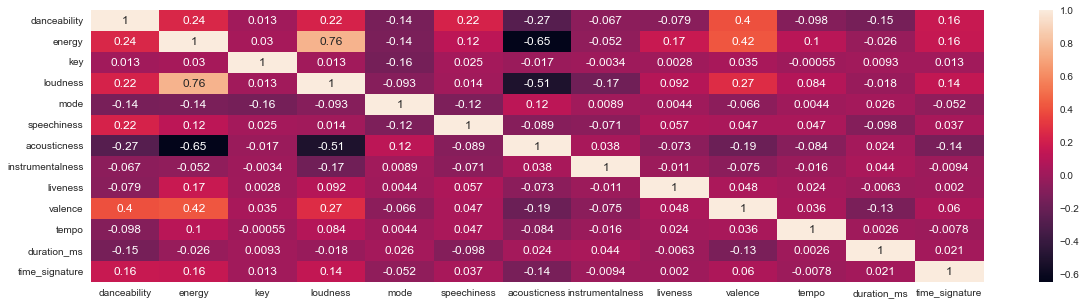
\includegraphics[width=\textwidth]{Outputs/Correlation Heatmap - Normalised Audio Features.png}}
\caption{Heatmap of correlations between the 13 normalised audio features}
\end{figure}

\subsection{Trends}
A time series analysis is performed exclusively on the  \textit{global} region of the dataset to see whether there is a weekly or monthly seasonality. Instead of analysing each region separately, the \textit{global} region is chosen because it compiles all listening trends worldwide. By adding up the streams of the top 200 songs for a given day, the global region data of the top 200 streams each day are transformed into the total number of streams per day. An additive model is used as the change in trend is independent of its value. We discover a weekly seasonality where the daily streams fluctuate on an average of 50,000 between weekdays and weekends after being broken down into trend, seasonality, and noise. This represents a 5\% fluctuation in the steams, and this finding indicates that, on average, people's listening preferences shift over the weekends.
\begin{figure}[h]
\centering
\vstretch{0.9}{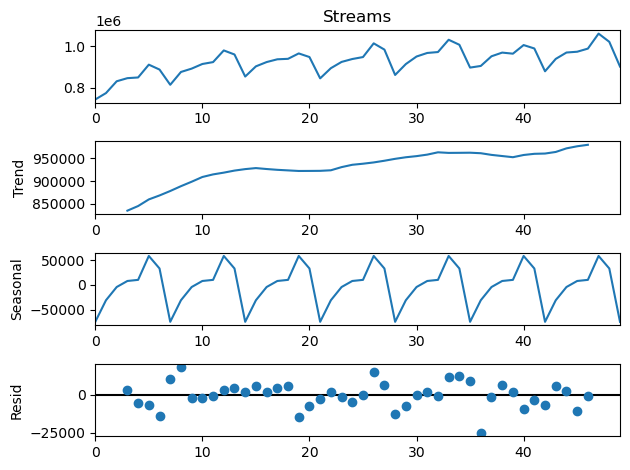
\includegraphics[width=0.5\linewidth]{Outputs/Trend.png}}
\caption{Seasonality of songs in the global region}
\end{figure}
\section{Learning Methods}
\subsection{Dimensionality Reduction}
It takes a lot of computing power to process and interpret high-dimensional data. The data experiences the so-called \textit{curse of dimensionality}, becoming sparser as the size of the feature space expands. By projecting features onto lower-dimensional subspaces and learning from them, dimensionality reduction techniques aid in the retention of the most relevant information and improve visualisation. In this section, we experiment with several manifold and projection based learning strategies. Even while they are effective, linear dimension reduction frameworks frequently overlook significant non-linear structures in the data, which manifold learning is more sensitive to and can better generalise. We analyse the clustering outcomes of the below approaches to see which yields the best results using the original dataset with its 13 attributes as our baseline.

\subsubsection{Methods}
\textbf{PCA} - is a standard approach for linear dimensionality reduction. We fit PCA on the normalised audio features and chose the number of components that produce 95\% of the cumulative explained variance, which in our case is 7. The visualisation for this is included in Appendix \ref{appendix:B}.

\textbf{UMAP} - is a non-linear manifold learning-based method that preserves the topological structure of points in a high-dimensional space in a lower-dimensional embedding space and employs Riemannian geometry to demonstrate the connectedness of related data points as clusters. All data points are grouped based on similarities in feature values, and similar groups are positioned closer. These are the local and global structures of the map. While UMAP is a great tool for generating visualisations, we use it more generally as a data transformer \cite{umap}. While \textit{min\_dist} is the minimal distance that controls how closely or loosely the clusters will be grouped in the low dimensional space, the parameter \textit{n\_neighbors} governs the number of neighbouring data points that define the local structures of the data in the feature space. 15 nearest neighbours are considered for our scaled audio features data set at a distance of 0.1 using the default \textit{n\_components}, 2. We also perform a grid search over these hyperparameters. The choice of the results is explained in Appendix \ref{appendix:B}.

\textbf{Gaussian Random Projection} - by exchanging a controllable amount of accuracy as additional variance for quicker processing times and smaller model sizes, the \textit{random\_projection} module of the \textit{scikit-learn} library implements a straightforward and computationally effective method for reducing the dimensionality of data \cite{randomprojections}. The Johnson-Lindenstrauss lemma is the primary theoretical finding that underlies the effectiveness of random projection. The lemma infers conclusions regarding low-distortion embeddings of points from high-dimensional into low-dimensional Euclidean space such that the distances between the points are almost preserved. The Gaussian Random Projection lowers the dimensionality by mapping the initial input space onto a randomly generated matrix, whose elements are selected from the following distribution - $N(0,\frac{1}{n\_{components}})$\cite{randomprojectionssklearn}. We set \textit{n\_components} to 2.

\textbf{PaCMAP} - in contrast to earlier manifold-based dimensionality reduction algorithms that either emphasise retaining local or global trends, PaCMAP with the correct settings can represent both equally. It uses three different types of pairs of data points: neighbour pairs (\textit{pair\_neighbors}), mid-near pairs (\textit{pair\_MN}), and further pairs (\textit{pair\_FP}) \cite{pacmap}. These values determine the number of closest neighbours to take into account, the proportion of mid-near pairs to the number of neighbours, and the proportion of further pairs to the number of neighbours, respectively. The feature space is transformed using PaCMAP with its default parameter values for \textit{n\_neighbours}, 10 and number of components, 2. The scaled audio feature values are then fit into this new space.

\textbf{Autoencoders} - are a class of neural networks that learn representations from data in an unsupervised manner and are typically used for dimensionality reduction and data regeneration. They consist of two primary components, an encoder and a decoder, each of which is represented by a family of parameterised functions - the encoder family ${\displaystyle E_{\math{\phi}}:{\mathcal{X}}\rightarrow {\mathcal{Z}}}$, parameterised by ${\displaystyle\math{\phi}}$ and the decoder family ${\displaystyle D_{\math{\theta}}:{\mathcal {Z}}\rightarrow {\mathcal {X}}}$, parameterised by ${\displaystyle \math{\theta}}$. The encoder maps features from a high dimensional data space ${\displaystyle\mathcal{X}}$ to a low dimensional latent space ${\displaystyle\mathcal{Z}}$ \cite{autoencoders}. The feed-forward architecture of our symmetrical autoencoder model is made of up two layers. A fully linked dense layer, a batch normalisation layer, and the Leaky ReLU activation function are all included in each portion of the encoder and decoder blocks. We restrict the bottleneck layer to 6 dimensions and train the model on the scaled audio features. The latent feature vector produced by the encoder - ${\displaystyle z=E_{\math{\phi} }(x)}$ is then used for clustering.

\subsection{Clustering}
\subsubsection{Methods}
We are able to represent the audio characteristics of the songs using the various sets of extracted features from the dimensionality reduction techniques outlined above. We compare the performance of three clustering algorithms: K-Means, DBSCAN, and BIRCH, on these new features and the original non-reduced dataset with 13 audio features. The clustering results for the various methods are included in Appendix \ref{appendix:C}.

\textbf{K-Means} - is an effective unsupervised machine learning algorithm that divides \textit{n} observations into \textit{k} clusters, each containing points that belong to the closest mean (also known as the cluster centroid and functions as the cluster's prototype). As a result, the data space gets partitioned into several Voronoi cells \cite{kmeans}. The algorithm minimises within-cluster variances (squared Euclidean distances), termed named inertia. We use the \textit{k-means++} initialisation approach provided by \textit{scikit-learn} library to position the centroids far apart from one another. Since the euclidean distance is explosive in high-dimensional spaces, we reason that K-Means will adapt and scale well and efficiently to our implementations using dimensionality reduction. We use the Elbow method with distortion scores to determine the optimal number of clusters for each feature set.

The knee of the elbow plot is where adding a new cluster does not enhance the quality of the existing ones; and rather leads to overfitting. This strategy provides us with a sufficient number of clusters to use for each of the feature extraction strategies, as seen in \ref{fig:elbowplots}, with sizes mostly varying between 8 and 13.

\begin{figure}[!hbt]
\begin{subfigure}{.5\textwidth}
  \centering
  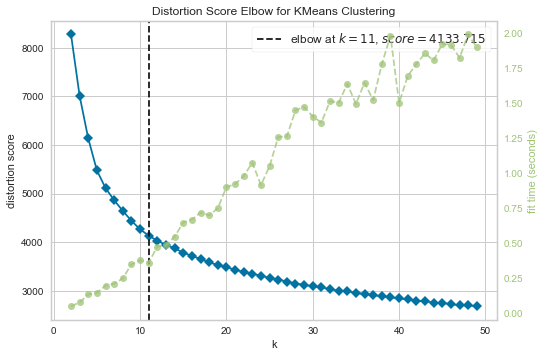
\includegraphics[width=.6\linewidth]{Outputs/Elbow Plot - Original Audio Features.png}  
  \captionsetup{justification=centering,margin=1cm}
  \caption{Number clusters for the original audio features}
  \label{fig:sub-first}
\end{subfigure}
\begin{subfigure}{.5\textwidth}
  \centering
  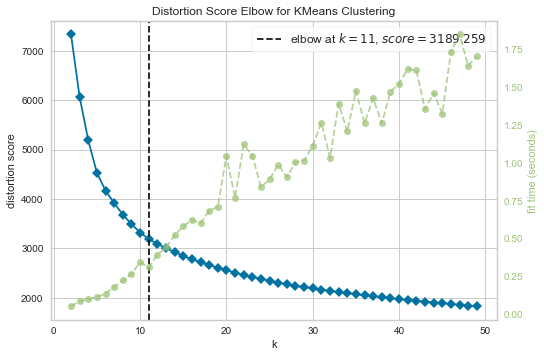
\includegraphics[width=.6\linewidth]{Outputs/Elbow Plot - PCA Features.png}  
  \captionsetup{justification=centering,margin=1cm}
  \caption{Number of clusters for the PCA audio features}
  \label{fig:sub-second}
\end{subfigure}
\medskip
\begin{subfigure}{.5\textwidth}
  \centering
  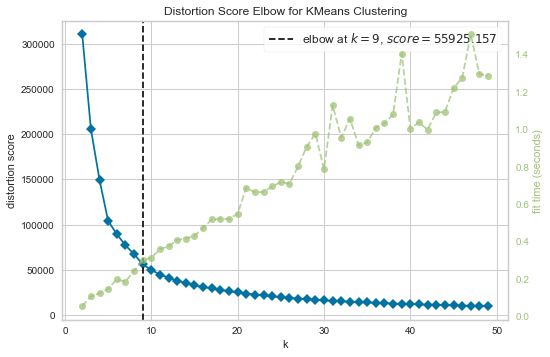
\includegraphics[width=.6\linewidth]{Outputs/Elbow Plot - UMAP Features.png}  
  \captionsetup{justification=centering,margin=1cm}
  \caption{Number of clusters for UMAP audio features}
  \label{fig:sub-third}
\end{subfigure}
\begin{subfigure}{.5\textwidth}
  \centering
  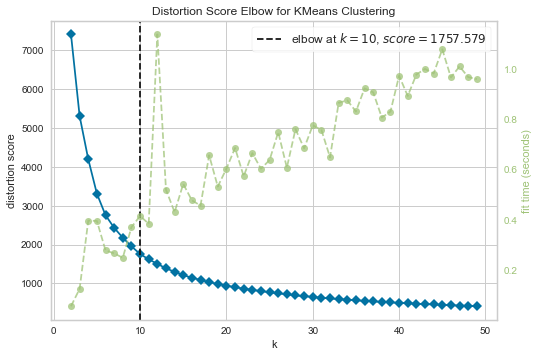
\includegraphics[width=.6\linewidth]{Outputs/Elbow Plot - Gaussian Random Projections.png} 
  \captionsetup{justification=centering,margin=1cm}
  \caption{Number of clusters for the Gaussian Random Projection audio features}
  \label{fig:sub-fourth}
\end{subfigure}
\medskip
\begin{subfigure}{.5\textwidth}
  \centering
  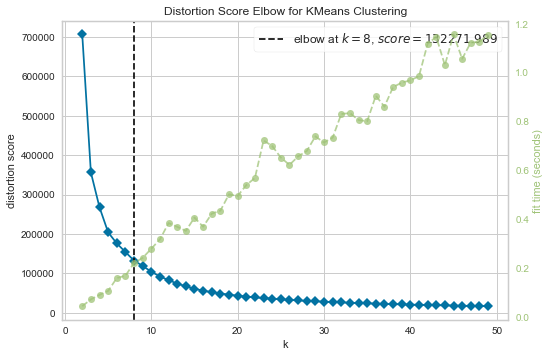
\includegraphics[width=.6\linewidth]{Outputs/Elbow Plot - PaCMAP Features.png} 
  \captionsetup{justification=centering,margin=1cm}
  \caption{Number of clusters for the PaCMAP audio features}
  \label{fig:sub-fifth}
\end{subfigure}
\begin{subfigure}{.5\textwidth}
  \centering
  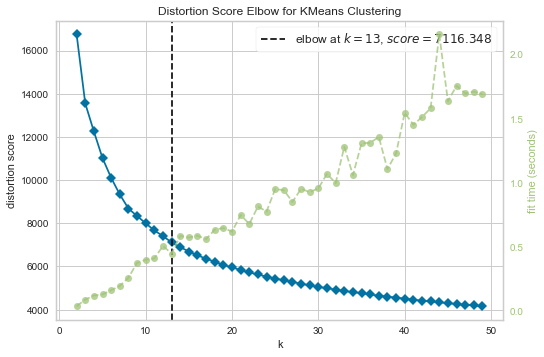
\includegraphics[width=.6\linewidth]{Outputs/Elbow Plot - Autoencoder Features.png}  
  \captionsetup{justification=centering,margin=1cm}
  \caption{Number of clusters for the Autoencoder audio features}
  \label{fig:sub-sixth}
\end{subfigure}
\caption{Elbow plots representing the optimal number of clusters with various dimensionality reduction algorithms for K-Means}
\label{fig:elbowplots}
\end{figure}
\setlength{\textfloatsep}{5pt}
\textbf{DBSCAN} - is a density-based clustering algorithm. The underlying concept is that a cluster in data space is viewed as a contiguous zone of high point density that is removed from other similar clusters by continuous regions of low point density. It can find clusters of various sizes and forms from data that contains vast amounts of noise and outliers. The two main parameters of the algorithm, \textit{min\_samples} and \textit{eps}, are what give us this notion of density. Higher \textit{min\_samples} or lower \textit{eps} imply a cluster requires a higher density to develop. As opposed to \textit{min\_pts}, which specifies the minimum number of neighbours required to create a cluster, \textit{eps} reflects the minimal distance between points for them to be regarded as neighbours. We perform a grid search on these parameters for each of the feature sets obtained from the dimensionality reduction step. Details are included in Appendix \ref{appendix:B}.

\textbf{BIRCH} - stands for Balanced Iterative Reducing and Clustering using Hierarchies and involves scanning local regions of the feature space to form hierarchical Clustering-Feature trees before expanding to create clusters throughout the entire data set. These CF trees contain a condensed summary of the main feature set, which are then clustered globally. As BIRCH only works with metric attributes or features that can be represented in the euclidean space, our audio features fit that requirement. Its parameter \textit{n\_clusters} is set to \textit{None} to allow the algorithm to run and determine the sub-clusters without performing the final clustering step.

\subsubsection{Metrics}
\textbf{Silhouette Score} - is calculated using the mean intra-cluster distance (a) and the mean nearest-cluster distance (b) for each sample as $(b-a)/max(a,b)$. The ideal value is 1, whereas -1 is undesirable. Values close to 0 signify clusters that overlap while negative results typically signify that a sample is placed in the incorrect cluster because another cluster would have better fit the sample.

\textbf{Calinski-Harabasz Score} - is another metric used to assess the performance of the clustering methods on the different reduced feature sets. It calculates a ratio of the sum of inter-cluster dispersion and the sum of intra-cluster squared distances for all clusters. A higher CH Index represents tightly clustered data that is well separated from the other clusters \cite{ch}.

\textbf{Davies-Bouldin Index} - is a metric that calculates the average similarity of each cluster to its most similar cluster, where the average similarity is also measured as the ratio of within-cluster distances to between-cluster distances. The lower this index value, the better separated are the clusters \cite{dbi}.
\section{Results}
The CH, DB, and SS scores given in Table \ref{tab:results} are the results of several clustering algorithms using various dimensionality reduction techniques. These are evaluated against a baseline model that makes use of the 13 scaled audio properties and greatly surpasses it. These searches lead to the conclusion that the K-Means with PaCMAP is the best model, with the CH, DB, and SS scores coming in at 86258.97, 0.792, and 0.431, respectively. From the overall viewpoint of the clustering results, we discover that DBSCAN is ineffective because many of the data points are labelled as noise or outliers and given the value -1. The points are closely packed although the number of clusters itself is small in cases where the silhouette scores are $\approx0.3$. On the other hand, BIRCH returns the number of sub-clusters, in some cases, more than 100, with only a few song samples belonging to a given class. K-Means has a fair balance in this area between the number of clusters and the goodness of the clustering. The original un-scaled dataset with 13 audio features has a column added with the K-Means clustering labels generated by PaCMAP. We do not know what these clusters represent, even though our experiments have thus far discussed the approaches used for clustering. For each of the cluster labels, we draw a univariate analysis (a grid-map of histograms) for the 13 audio attributes to determine this. The findings and the visualisations are covered in Appendix \ref{appendix:D}. Since the clustering is done for the tracks rather than the artists, One artist could have appeared in more than one cluster because they may have created songs belonging to different genres. We also keep track of how many times each artist is included in a particular cluster. Appendix \ref{appendix:E} contains an extract for this outcome with 30 randomly sampled artists. Using the data from this table as an added feature to cluster artists together is one of the ideas for future implementations.

\begin{table}[hbt]
    \centering
    \rowcolors{1}{white}{gray!25}
    \resizebox{\columnwidth}{!}{%
    \begin{tabular}{|c|c|c|c|c|c|c|}
    \toprule
     \makecell{Clustering \\ Algorithm} & \makecell{Dimensionality \\ Reduction}  & \makecell{No. Clusters} & \makecell{No. Features} & 
     \makecell{CH} & \makecell{DB} & \makecell{SS} \\
    \midrule
        K-Means  & None (Baseline)      &  11      & 13     & 4987.08    & 1.796   & 0.163\\
        K-Means                   & PCA     &  11      & 7    & 6462.19   & 1.58  & 0.194\\
        K-Means                   & UMAP     &  9      & 2    & 97420.38   & 0.875  & 0.406\\
        K-Means                   & Gaussian Random Projection     &  10      & 2    & 20061.29  & 0.867  & 0.338\\
        \textbf{K-Means}                  & \textbf{PaCMAP}    &  \textbf{8}      & \textbf{2}    & \textbf{86258.97}   & \textbf{0.792}  & \textbf{0.431}\\
        K-Means                   & Autoencoder     &  13      & 6    & 16738.36   & 1.496  & 0.186\\
    \midrule
        BIRCH                   & None (Baseline)      &  61      & 13     & 1138.03    & 1.56   & 0.131\\
        BIRCH                   & PCA     &  13      & 7    & 5258.34   & 1.58 & 0.199\\
        BIRCH                   & UMAP     &  180      & 2    & 43173.12   & 0.880  & 0.330\\
        BIRCH                   & Gaussian Random Projection     &  5      & 2    & 20726.05 & 0.919  & 0.353\\
        BIRCH                   & PaCMAP     &  260      & 2    & 96680.87  & 0.864  & 0.324\\
        BIRCH                   & Autoencoder     &  8      & 6    & 66726.78  & 1.089  & 0.331\\
    \midrule
        DBSCAN                   & None (Baseline)      &  5      & 13     & 3522.65    & 1.585   & 0.365\\
        DBSCAN                   & PCA     &  5     & 7    & 3706.69   & 1.829 & 0.191\\
        DBSCAN                   & UMAP     &  5      & 2    & 30712.09   & 1.899  & 0.161\\
        DBSCAN                   & Gaussian Random Projection     &  7      & 2    & 11.501 & 1.632  & 0.168\\
        DBSCAN                   & PaCMAP     &  5      & 2    & 26649.71  & 0.628  & 0.335\\
        DBSCAN                   & Autoencoder     &  3      & 6    & 36465.97  & 0.761  & 0.349\\
    \bottomrule
    \end{tabular}%
    }
    \caption{Experiment results for different combinations of clustering algorithms and dimensionality reduction methods. SS is silhouette score, DB is Davies–Bouldin index, CH is Calinski Harabasz score. Row in \textbf{bold} indicates the best model.}
    \label{tab:results}
\end{table} 
\vspace{-2em}
\section{Conclusions}
We explored several dimensionality reduction methods with clustering algorithms on the Spotify audio characteristics dataset. We concluded that the best results were obtained using K-Means with PaCMAP. We also tried extending the work partially to cluster songs based on their trajectories. The results are included in Appendix \ref{appendix:F}. We could evaluate the system with the help of other variations of K-Means like MiniBatchKMeans and weighted K-Means, or perhaps some agglomerative clustering methods. Currently we have the artists' song cluster signature on which we can run other clustering methods to group similar artists. Performing region-based clustering of artists to facilitate artist collaboration is one of the primary applications of this approach since different geographic areas around the world produce different types of sounds. Another task would be to train deep learning models like LSTMs to predict the trends of songs. 


\bibliography{refs.bib}
\bibliographystyle{plain}
\newpage
\section{Appendix}
\begin{appendix}
\section{Distribution of Audio Features}
\label{appendix:A}
We plotted the individual distributions of the original 13 audio features (a) and those features after normalisation (b) to check for any correlations between them
\begin{figure}[H]
\begin{subfigure}{1\textwidth}
\centering
    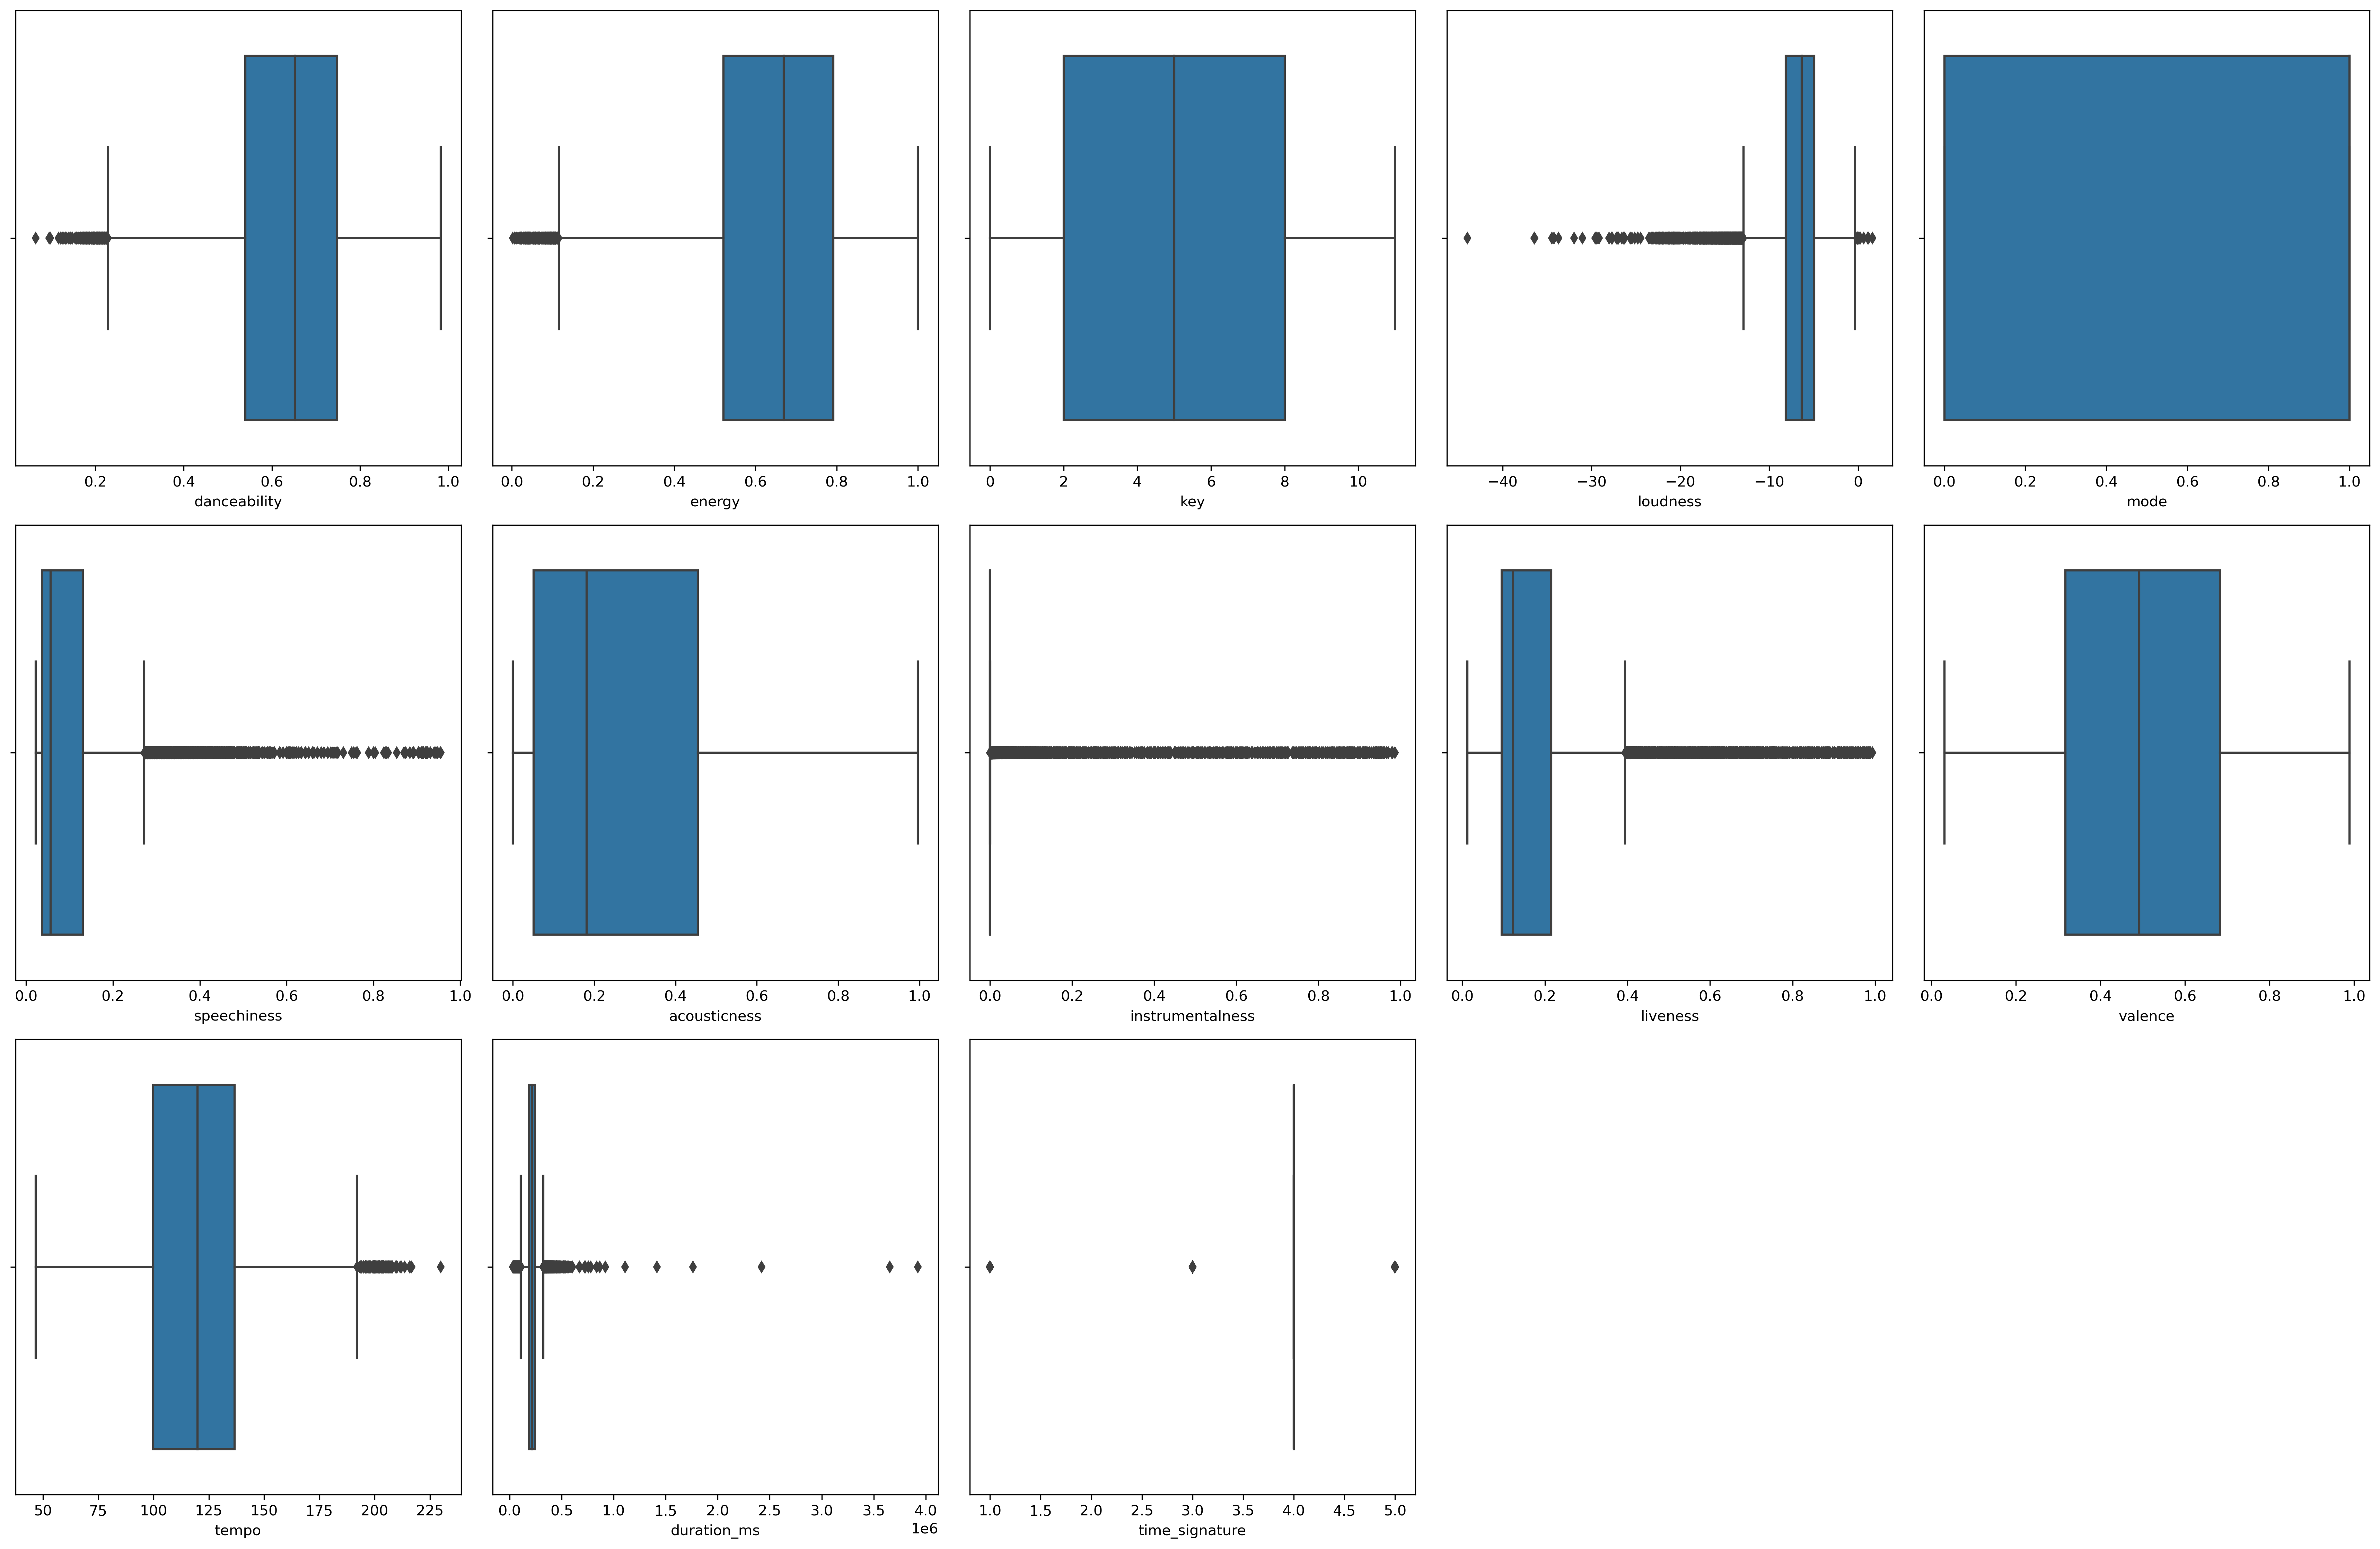
\includegraphics[scale=0.2]{Outputs/Boxplot - Original Audio Features.png}
    \captionsetup{justification=centering,margin=1cm}
    \caption{Boxplot of original audio features as retrieved from the Spotify API}
    \label{fig:sub-first}
\end{subfigure}
\newline
\begin{subfigure}{1\textwidth}
\centering
    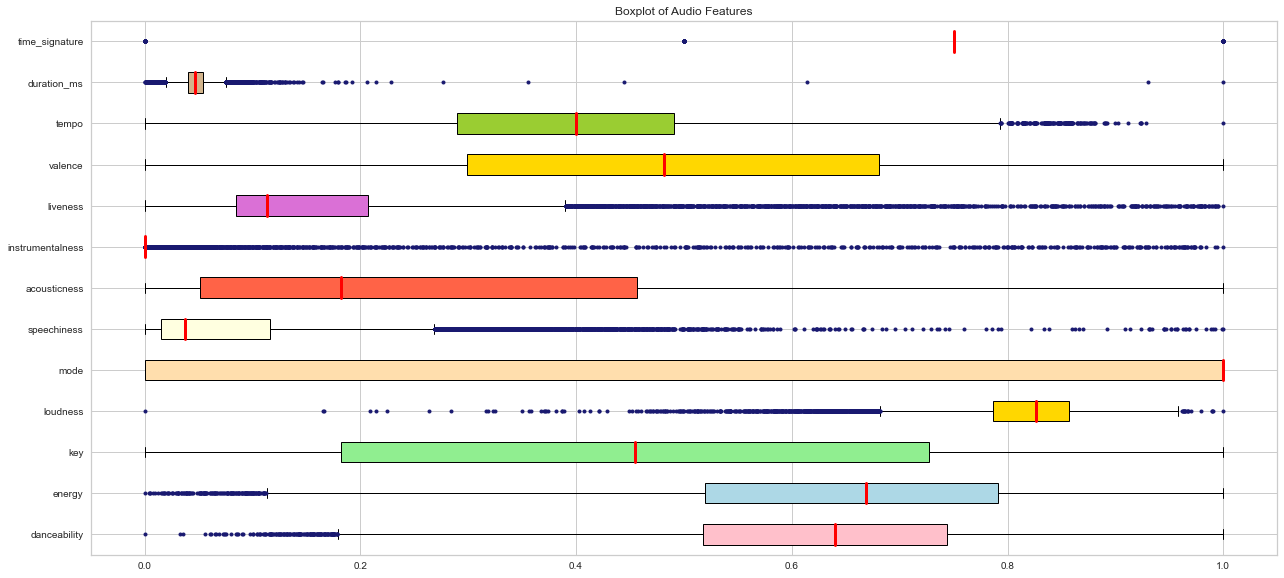
\includegraphics[scale=0.3]{Outputs/Boxplot - Normalised Audio Features.png}
    \captionsetup{justification=centering,margin=1cm}
    \caption{Boxplot of normalised audio features}
    \label{fig:sub-second}
\end{subfigure}
\end{figure}

\section{Dimensionality Reduction}
\label{appendix:B}
\subsection{PCA}
\begin{figure}[h!]
\centering
\centerline{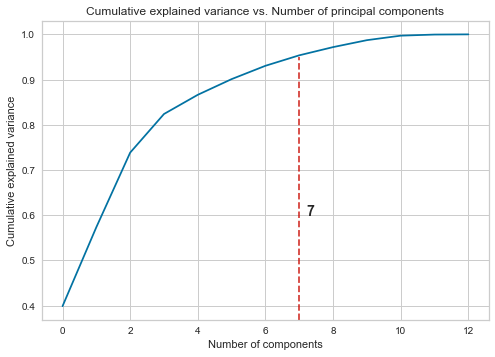
\includegraphics[scale=0.3]{Outputs/PCA - Number of Components.png}}
\captionsetup{justification=centering,margin=1cm}
\caption{Cumulative explained variance of PCA on the original dataset with 13 features. 7 components yield 95\% of the variance}
\end{figure}

\subsection{Grid Search for UMAP with K-Means}
Grid Search is an exhaustive hyperparameter tuning technique that helps in determining the optimal values of parameter combinations for a model. We created a pipeline to find the optimal number of clusters for K-Means with UMAP reduced audio features.

\newlength\dunder
\settowidth{\dunder}{\_}
The following parameters were used
\begin{table}
\begin{center}
\resizebox{\columnwidth}{!}{%
\begin{tabular}{cc|c|c|c|c|c}
\multicolumn{2}{c}{} & \multicolumn{5}{c}{} \\ \cline{3-6}
\multicolumn{2}{c|}{} & \texttt{umap\rule{2\dunder}{0.02pt}n\rule{1\dunder}{0.1pt}neighbors} &
\texttt{umap\rule{2\dunder}{0.02pt}min\rule{1\dunder}{0.1pt}dist} &
\texttt{umap\rule{2\dunder}{0.02pt}n\rule{1\dunder}{0.1pt}components} &
\texttt{kmeans\rule{2\dunder}{0.02pt}n\rule{1\dunder}{0.1pt}clusters} \\ \cline{3-6}
&&5&0.1&2&2& \\ \cline{3-6}
&&10&0.4&3&7& \\ \cline{3-6}
&&20&0.6&-&15& \\ \cline{3-6}
&&50&0.9&-&20& \\ \cline{3-6}
&&100&-&-&30& \\ \cline{3-6}
&&-&-&-&50& \\ \cline{3-6}
\end{tabular}%
}
\end{center}
\caption{Grid Search parameters for UMAP with K-Means}
\end{table}

The best parameters returned by the search were kmeans\rule{2\dunder}{0.02pt}n\rule{1\dunder}{0.1pt}clusters: 50, umap\rule{2\dunder}{0.02pt}min\rule{1\dunder}{0.1pt}dist: 0.1, umap\rule{2\dunder}{0.02pt}n\rule{1\dunder}{0.1pt}components: 2, umap\rule{2\dunder}{0.02pt}n\rule{1\dunder}{0.1pt}neighbors: 100

And the clustering results were as follows
\begin{figure}[h]
    \centering
    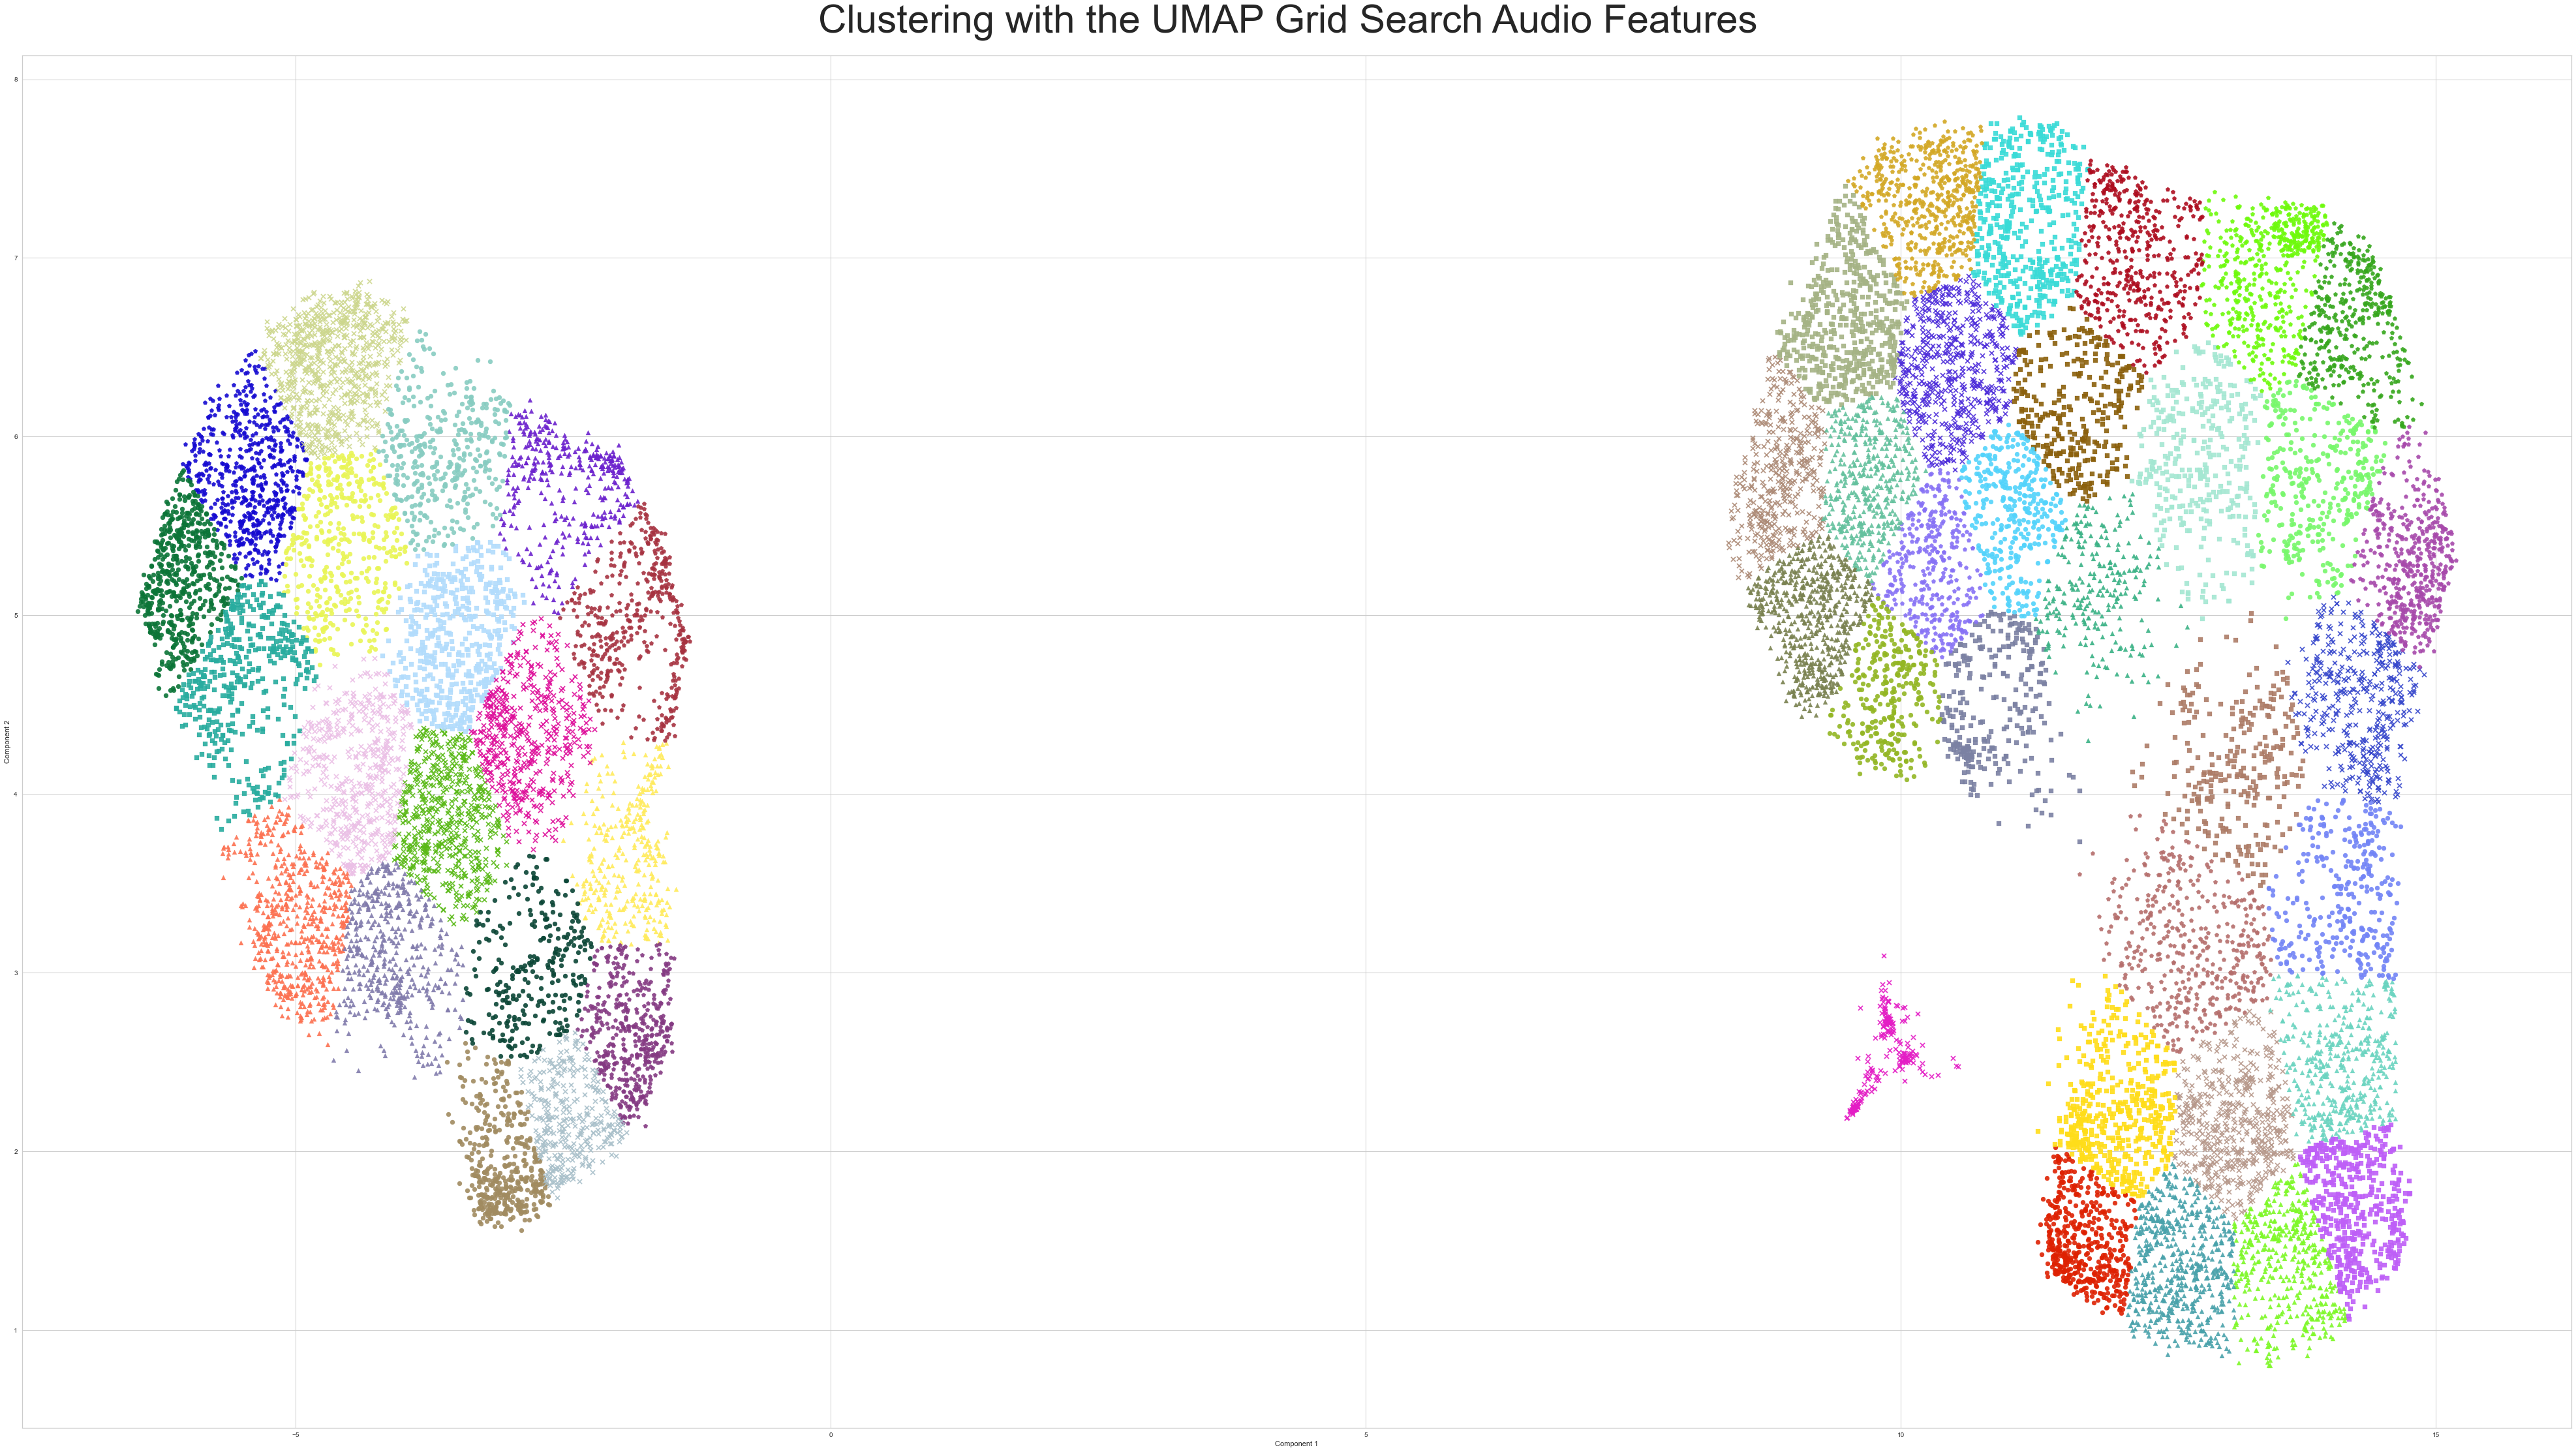
\includegraphics[scale=0.07]{Outputs/Cluestering - UMAP Grid Search Features.png}
    \caption{K-Means with UMAP derived features after Grid Search}
    \captionsetup{justification=centering,margin=1cm}
    \label{fig:kmeans-umap-gs}
\end{figure}

However, we chose not to go with the search results since 50 clusters are too fine-grained. Hence, we chose the number of clusters returned by the elbow curve.

\subsection{Silhouette Analysis for K-Means}
The success of the the K-Means clustering methods relies on an appropriately selected \textit{k} value or the number of clusters \textit{n\_clusters} to be formed. This number and the other parameters were empirically derived using heuristic methods including elbow plots as shown in the main section of the report above and silhouette analysis.

We experimented with K-Means \textit{n\_clusters} ranging from [2,50] and plotted the corresponding silhouette scores for clustering on features derived by each of the dimensionality reduction algorithms covered above. The optimal number of clusters for K-Means was found to be 2 or 3 based on the results from the majority of the methods. This measure didn't seem appropriate for this task because there weren't enough clusters to adequately capture the variation in the types of songs. Instead, this rating was used as an evaluation tool to contrast the different dimensionality reduction and clustering methods. Due to space constraints, the screenshots of the silhouette plots are not included here. However they can be found in the output cells of our code file \textit{'Spotify Data Analysis.ipynb'}

\subsection{Grid Search - DBSCAN}
We created our own grid search for the DBSCAN algorithm with the following parameters - $eps = [0.1, 0.2, 0.6, 0.8]$ and $min\_samples = [2, 4, 6, 8]$ and reported the Calinski Harabasz score, Davies Bouldin index, Silhouette scores and number of clusters for each combination. We chose the values for \textit{eps} and \textit{min\_samples} that gave us a moderate number of clusters (not too coarse or fine grained), and a good trade-off between the other metrics.
The best set of parameters for each of the dimensionality reductions methods used are reported as follows

\begin{table}
\begin{center}
\begin{tabular}{c|c|c|c|ccc}
\multicolumn{2}{c}{} & \multicolumn{5}{c}{} \\ \cline{3-4}
\multicolumn{2}{c|}{} & \texttt{eps} & \texttt{min\_samples} & \\ \cline{2-4}
& \texttt{Original Audio Features} & 0.6 & 2 & & & \\ \cline{2-4}
 & \texttt{PCA} & 0.2 & 8 & & & \\ \cline{2-4}
& \texttt{UMAP} & 0.2 & 8 & & & \\ \cline{2-4}
& \texttt{Gaussian Random Projections} & 0.2 & 2 & & & \\ \cline{2-4}
& \texttt{PaCMAP}  & 0.8 & 8 & & & \\ \cline{2-4}
& \texttt{Autoencoders}  & 0.6 & 2 & & & \\ \cline{2-4}
\end{tabular}
\end{center}
\caption{Grid Search best parameters for each dimensionality reduction method with DBSCAN}
\end{table}

\section{Clustering Results}
\label{appendix:C}
\subsection{K-Means}
\begin{figure}[h]
    \centering
    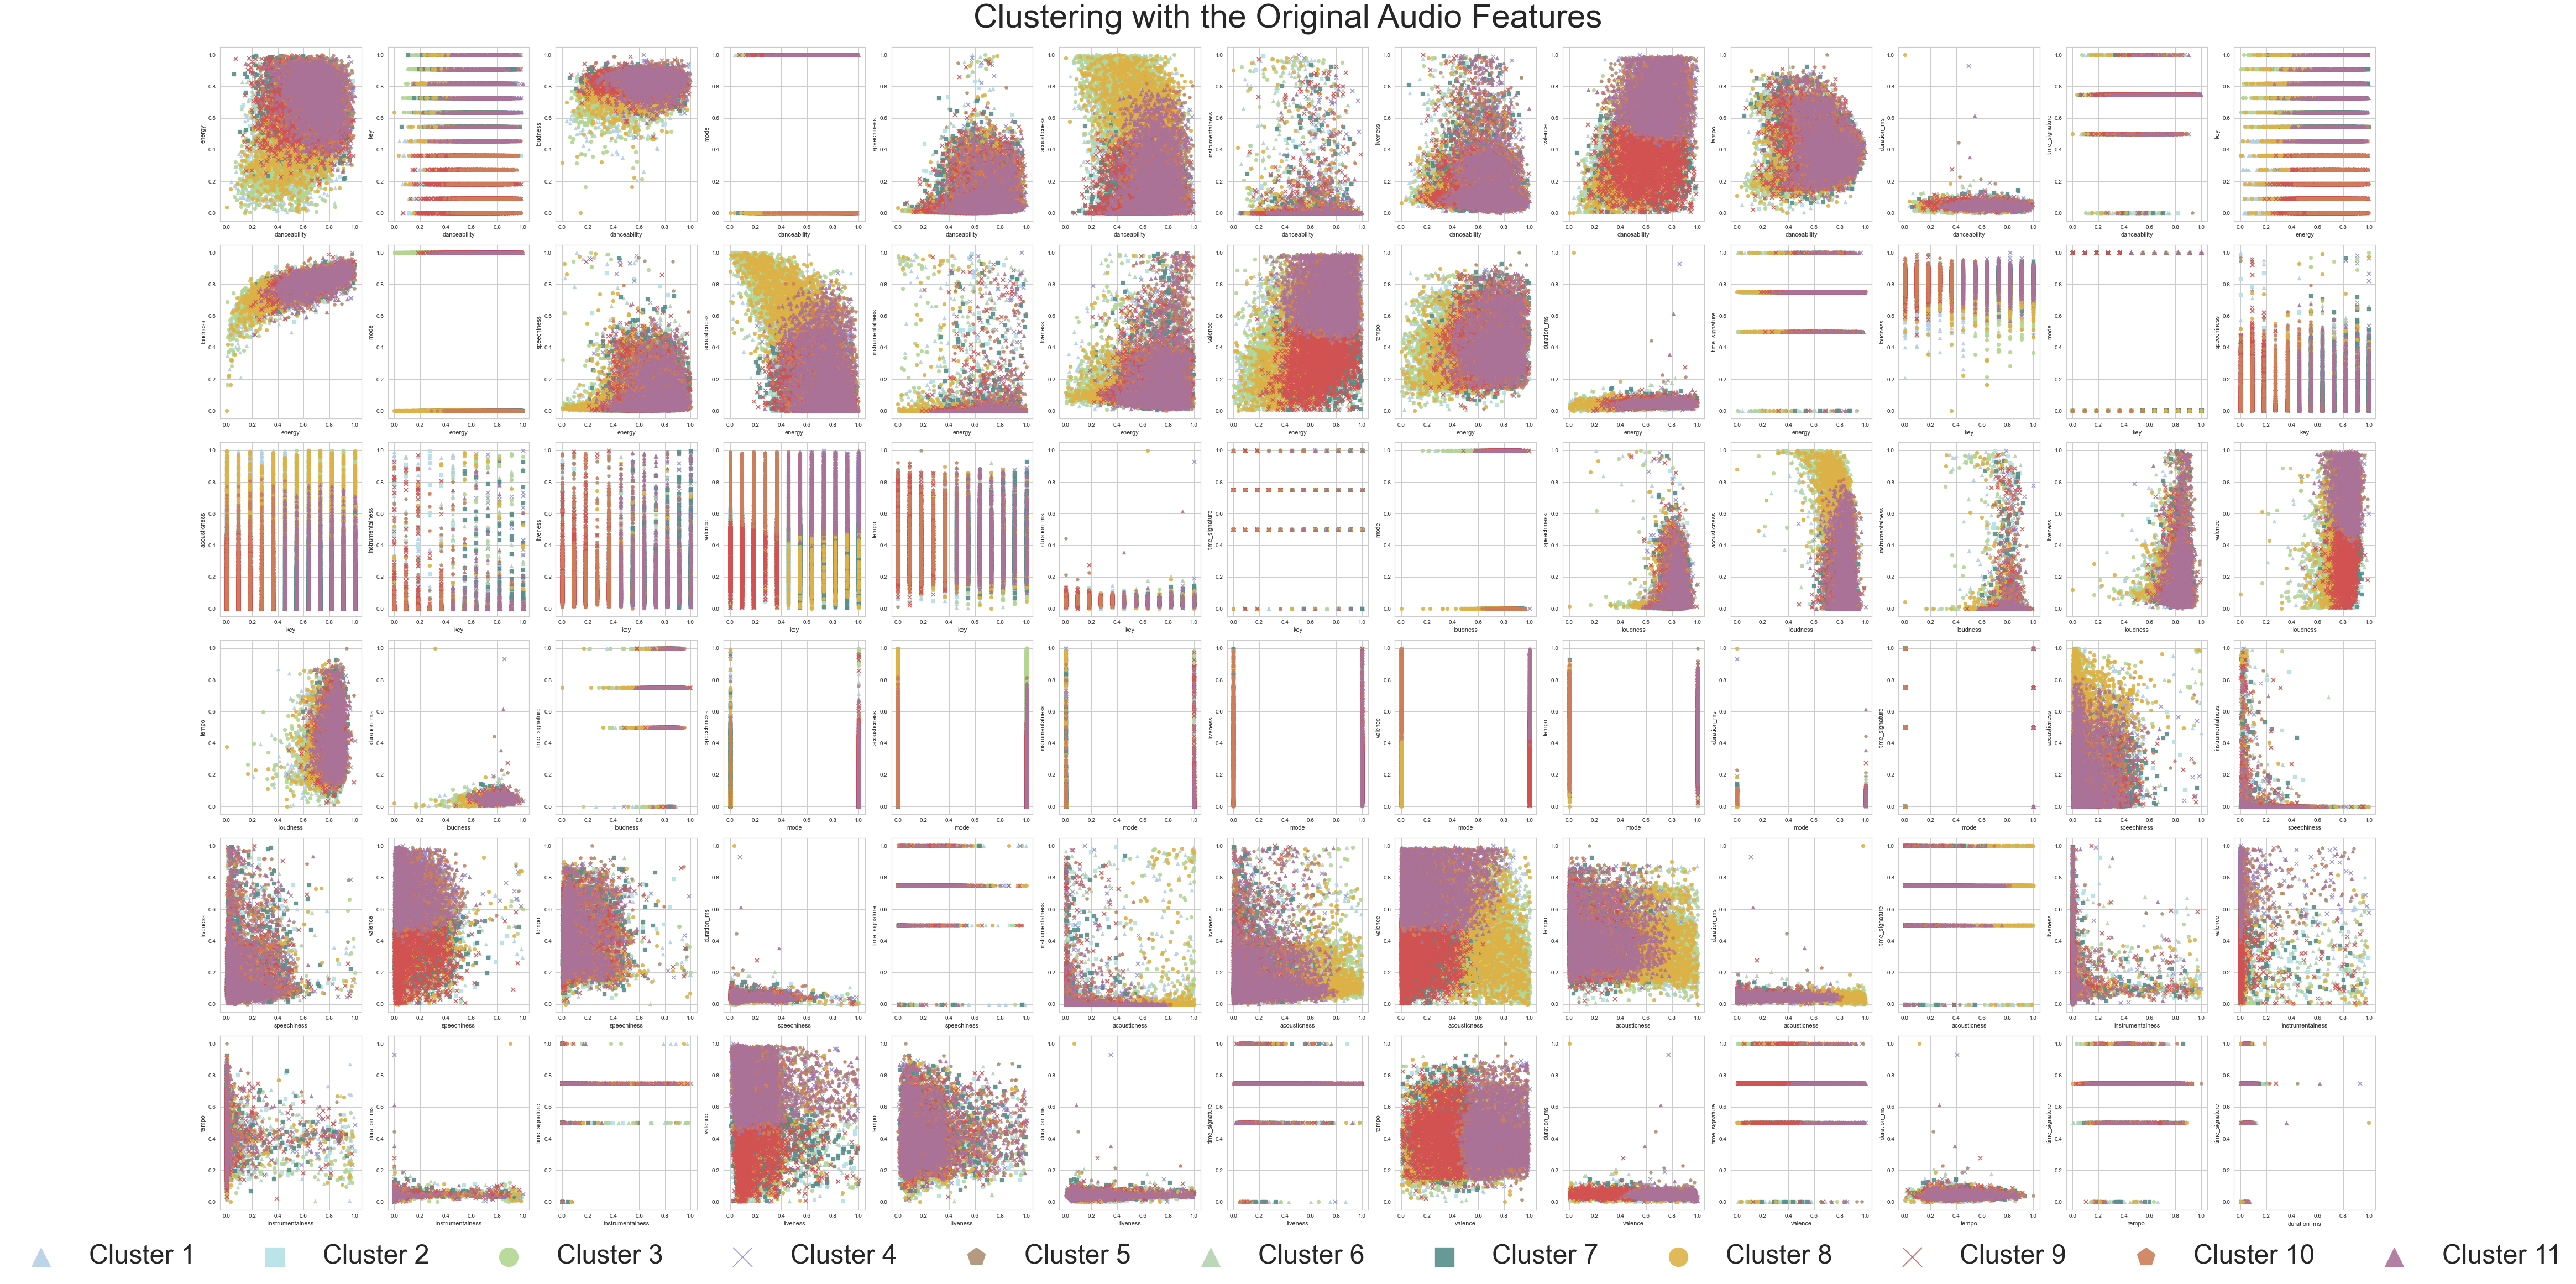
\includegraphics[scale=0.08]{Outputs/K-Means Clustering - Original Audio Features.png}
    \caption{K-Means clustering on the scaled original audio features}
    \label{fig:kmeans-first}
\end{figure}
\begin{figure}[!htb]
    \centering
    \includegraphics[scale=0.08]{Outputs/K-Means Clustering - PCA Audio Features.png}
    \caption{K-Means clustering on PCA dervived audio features}
    \label{fig:kmeans-second}
\end{figure}
\begin{figure}[!htb]
    \centering
    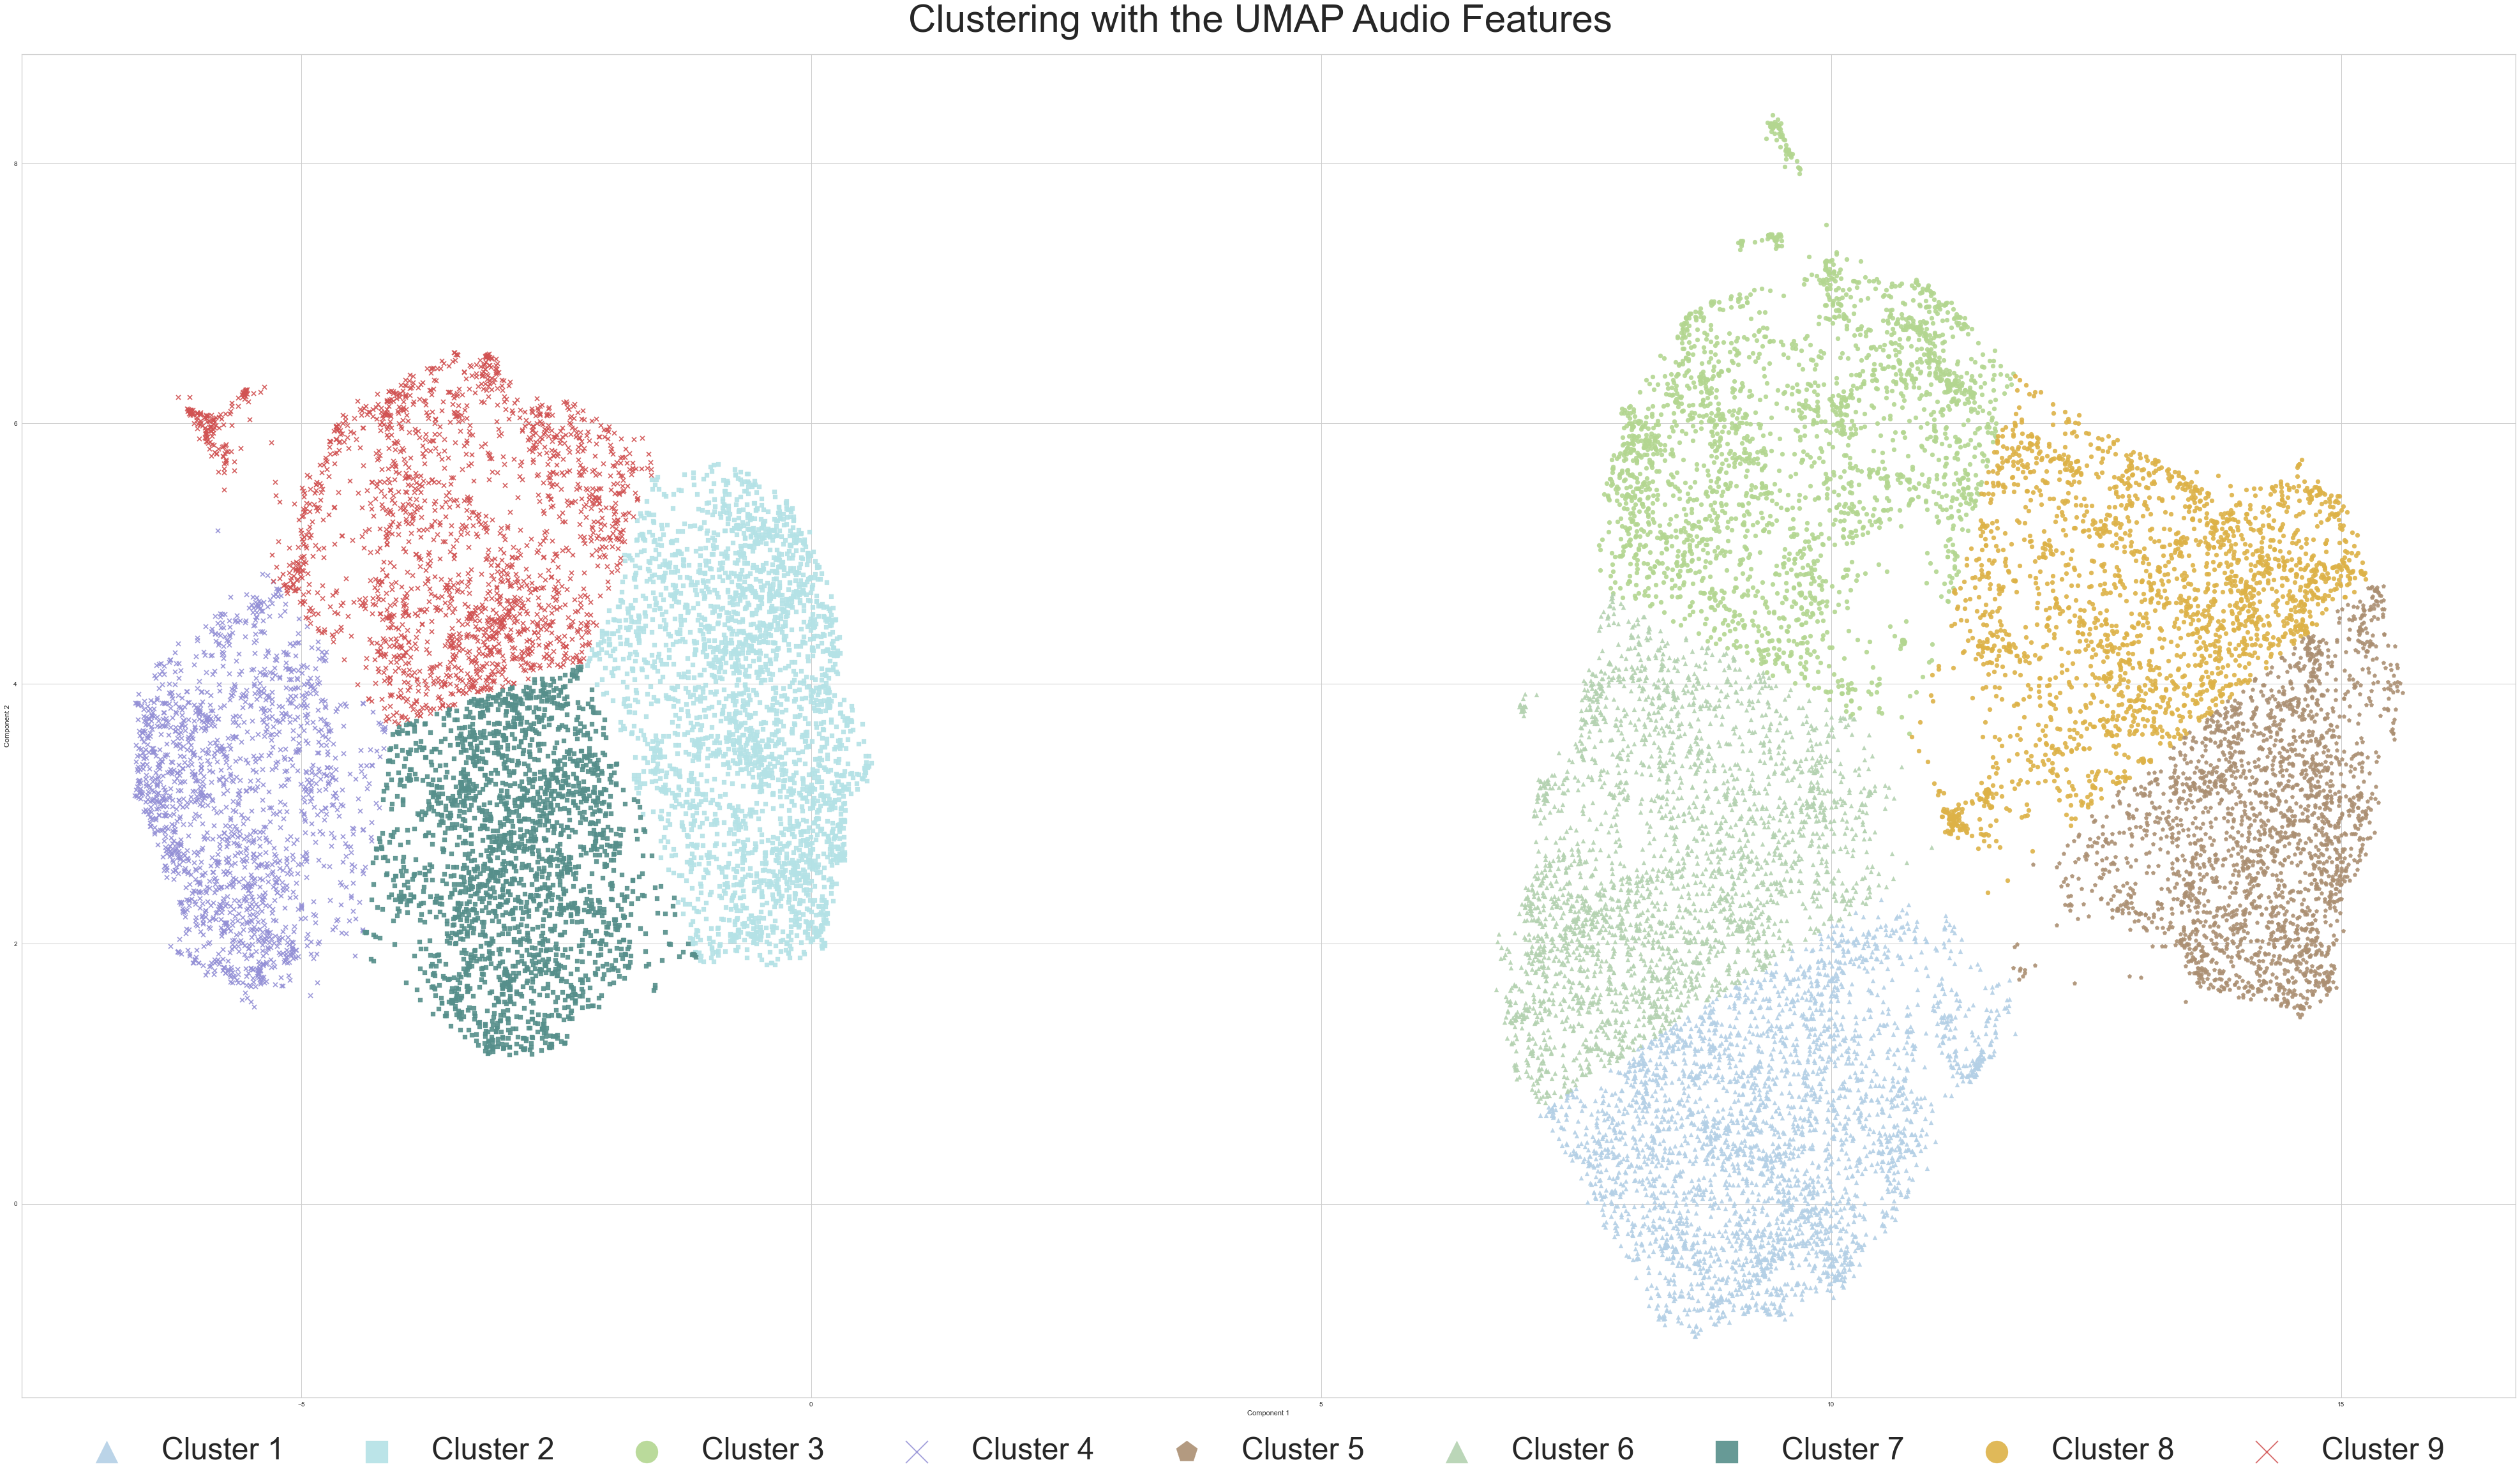
\includegraphics[scale=0.08]{Outputs/K-Means Clustering - UMAP Audio Features.png}
    \caption{K-Means clustering on UMAP derived audio features}
    \label{fig:kmeans-third}
\end{figure}
\begin{figure}[!htb]
    \centering
    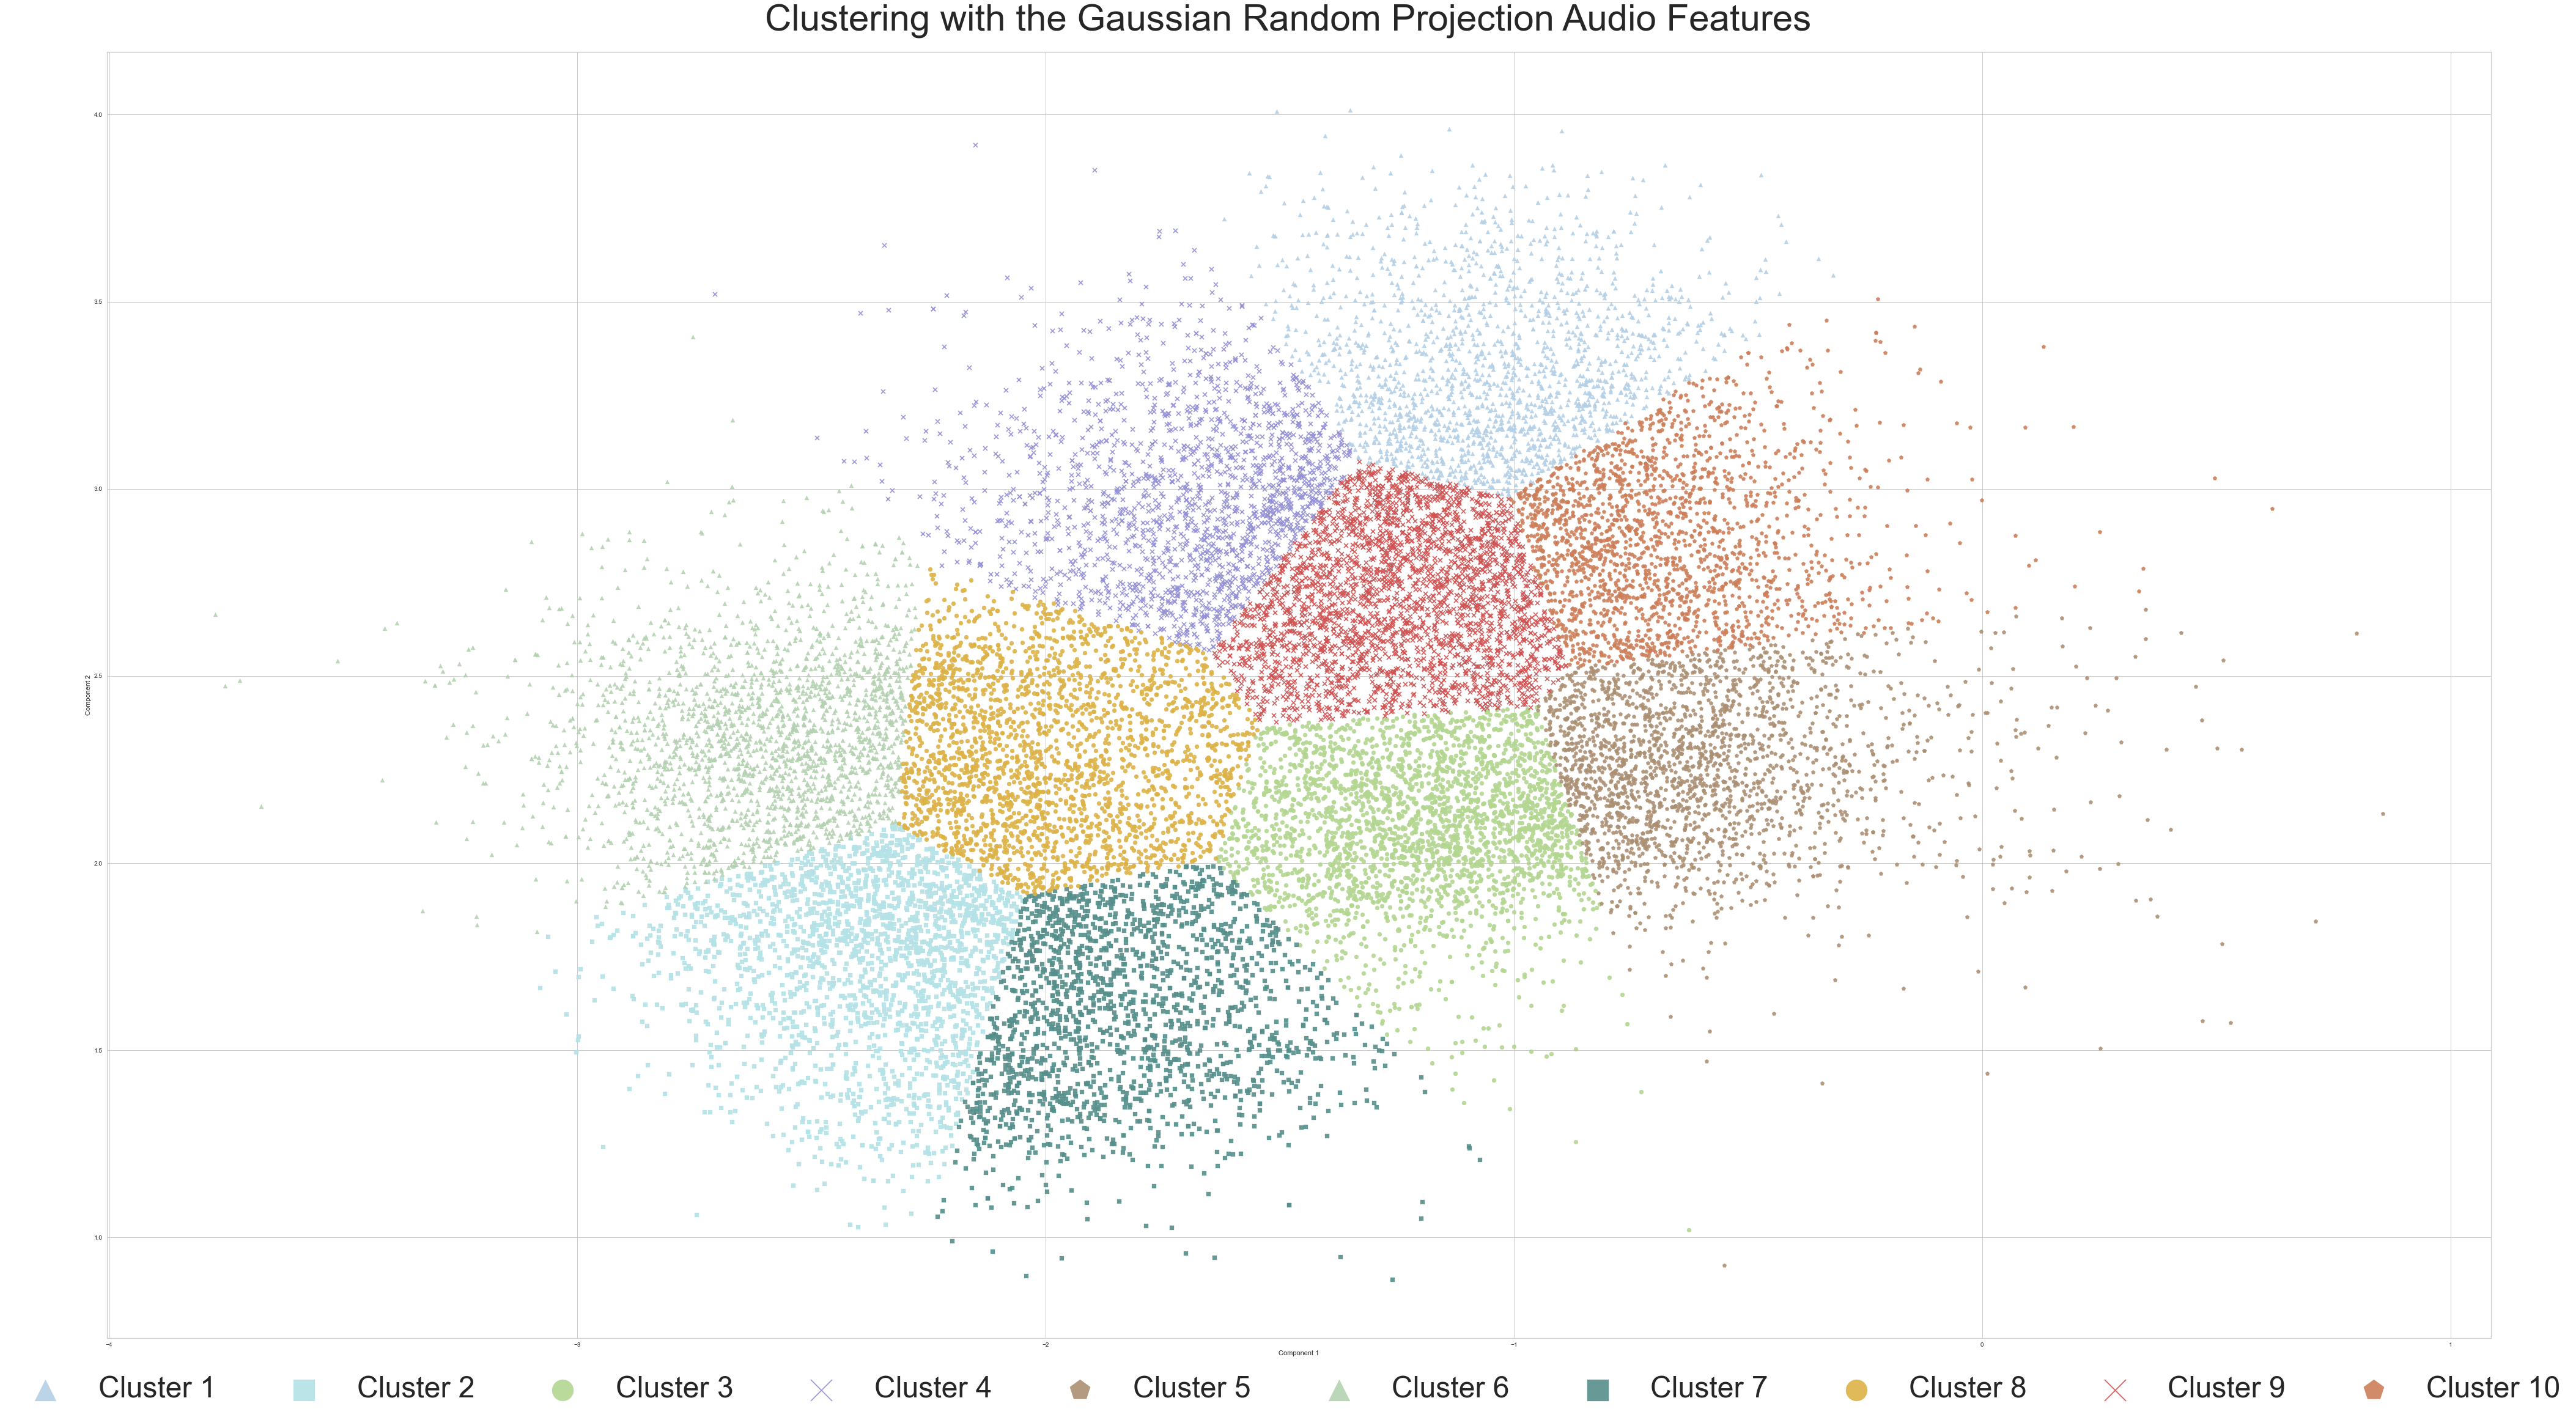
\includegraphics[scale=0.08]{Outputs/K-Means Clustering - Gaussian Random Projections Audio Features.png}
    \caption{K-Means clustering on Gaussian Random Projections derived audio features}
    \label{fig:kmeans-fourth}
\end{figure}
\begin{figure}[!htb]
    \centering
    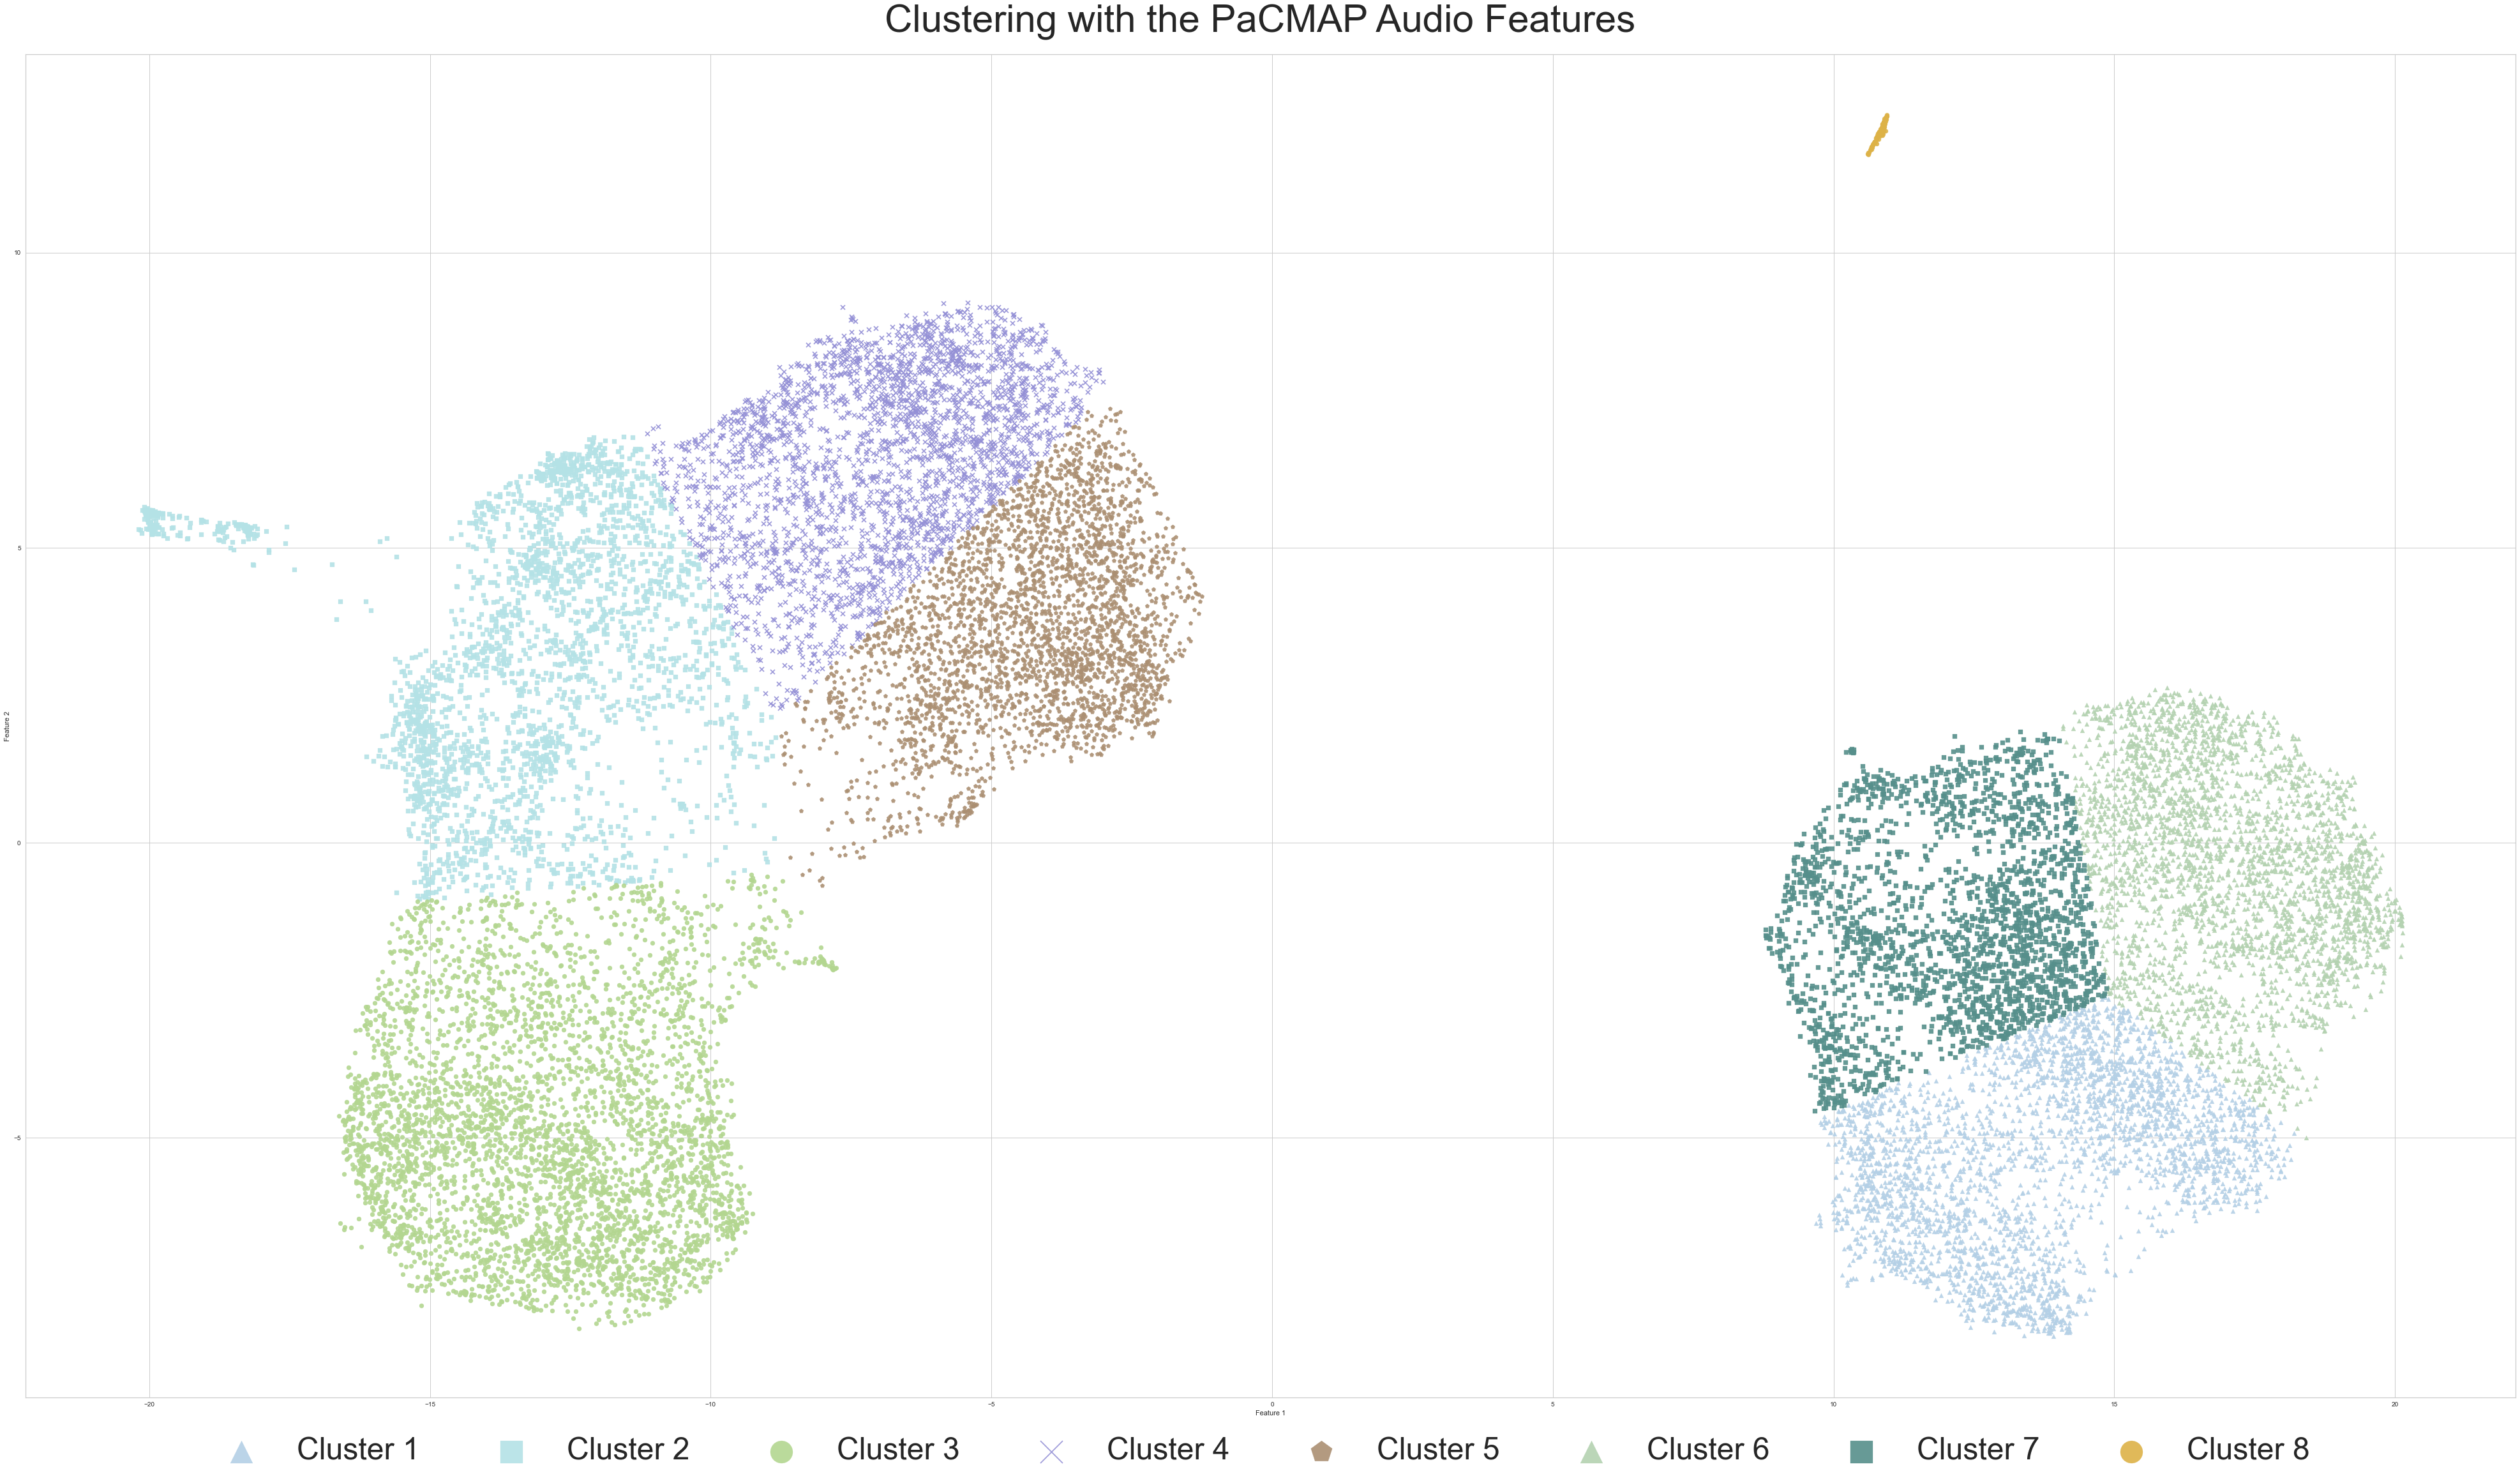
\includegraphics[scale=0.08]{Outputs/K-Means Clustering - PaCMAP Features.png}
    \caption{K-Means clustering on the PaCMAP derived audio features}
    \label{fig:kmeans-fifth}
\end{figure}
\begin{figure}[!htb]
    \centering
    \includegraphics[scale=0.07]{Outputs/K-Means Clustering - Autoencoder Audio Features.png}
    \caption{K-Means clustering on the Autoencoder derived audio features}
    \label{fig:kmeans-sixth}
\end{figure}
\FloatBarrier
\subsection{BIRCH}
\begin{figure}[!htb]
    \centering
    \includegraphics[scale=0.07]{Outputs/BIRCH Clustering - Original Audio Features.png}
    \caption{BIRCH clustering on the scaled original audio features}
    \label{fig:birch-first}
\end{figure}
\begin{figure}[!htb]
    \centering
    \includegraphics[scale=0.07]{Outputs/BIRCH Clustering - PCA Audio Features.png}
    \caption{BIRCH clustering on PCA dervived audio features}
    \label{fig:birch-second}
\end{figure}
\begin{figure}[!htb]
    \centering
    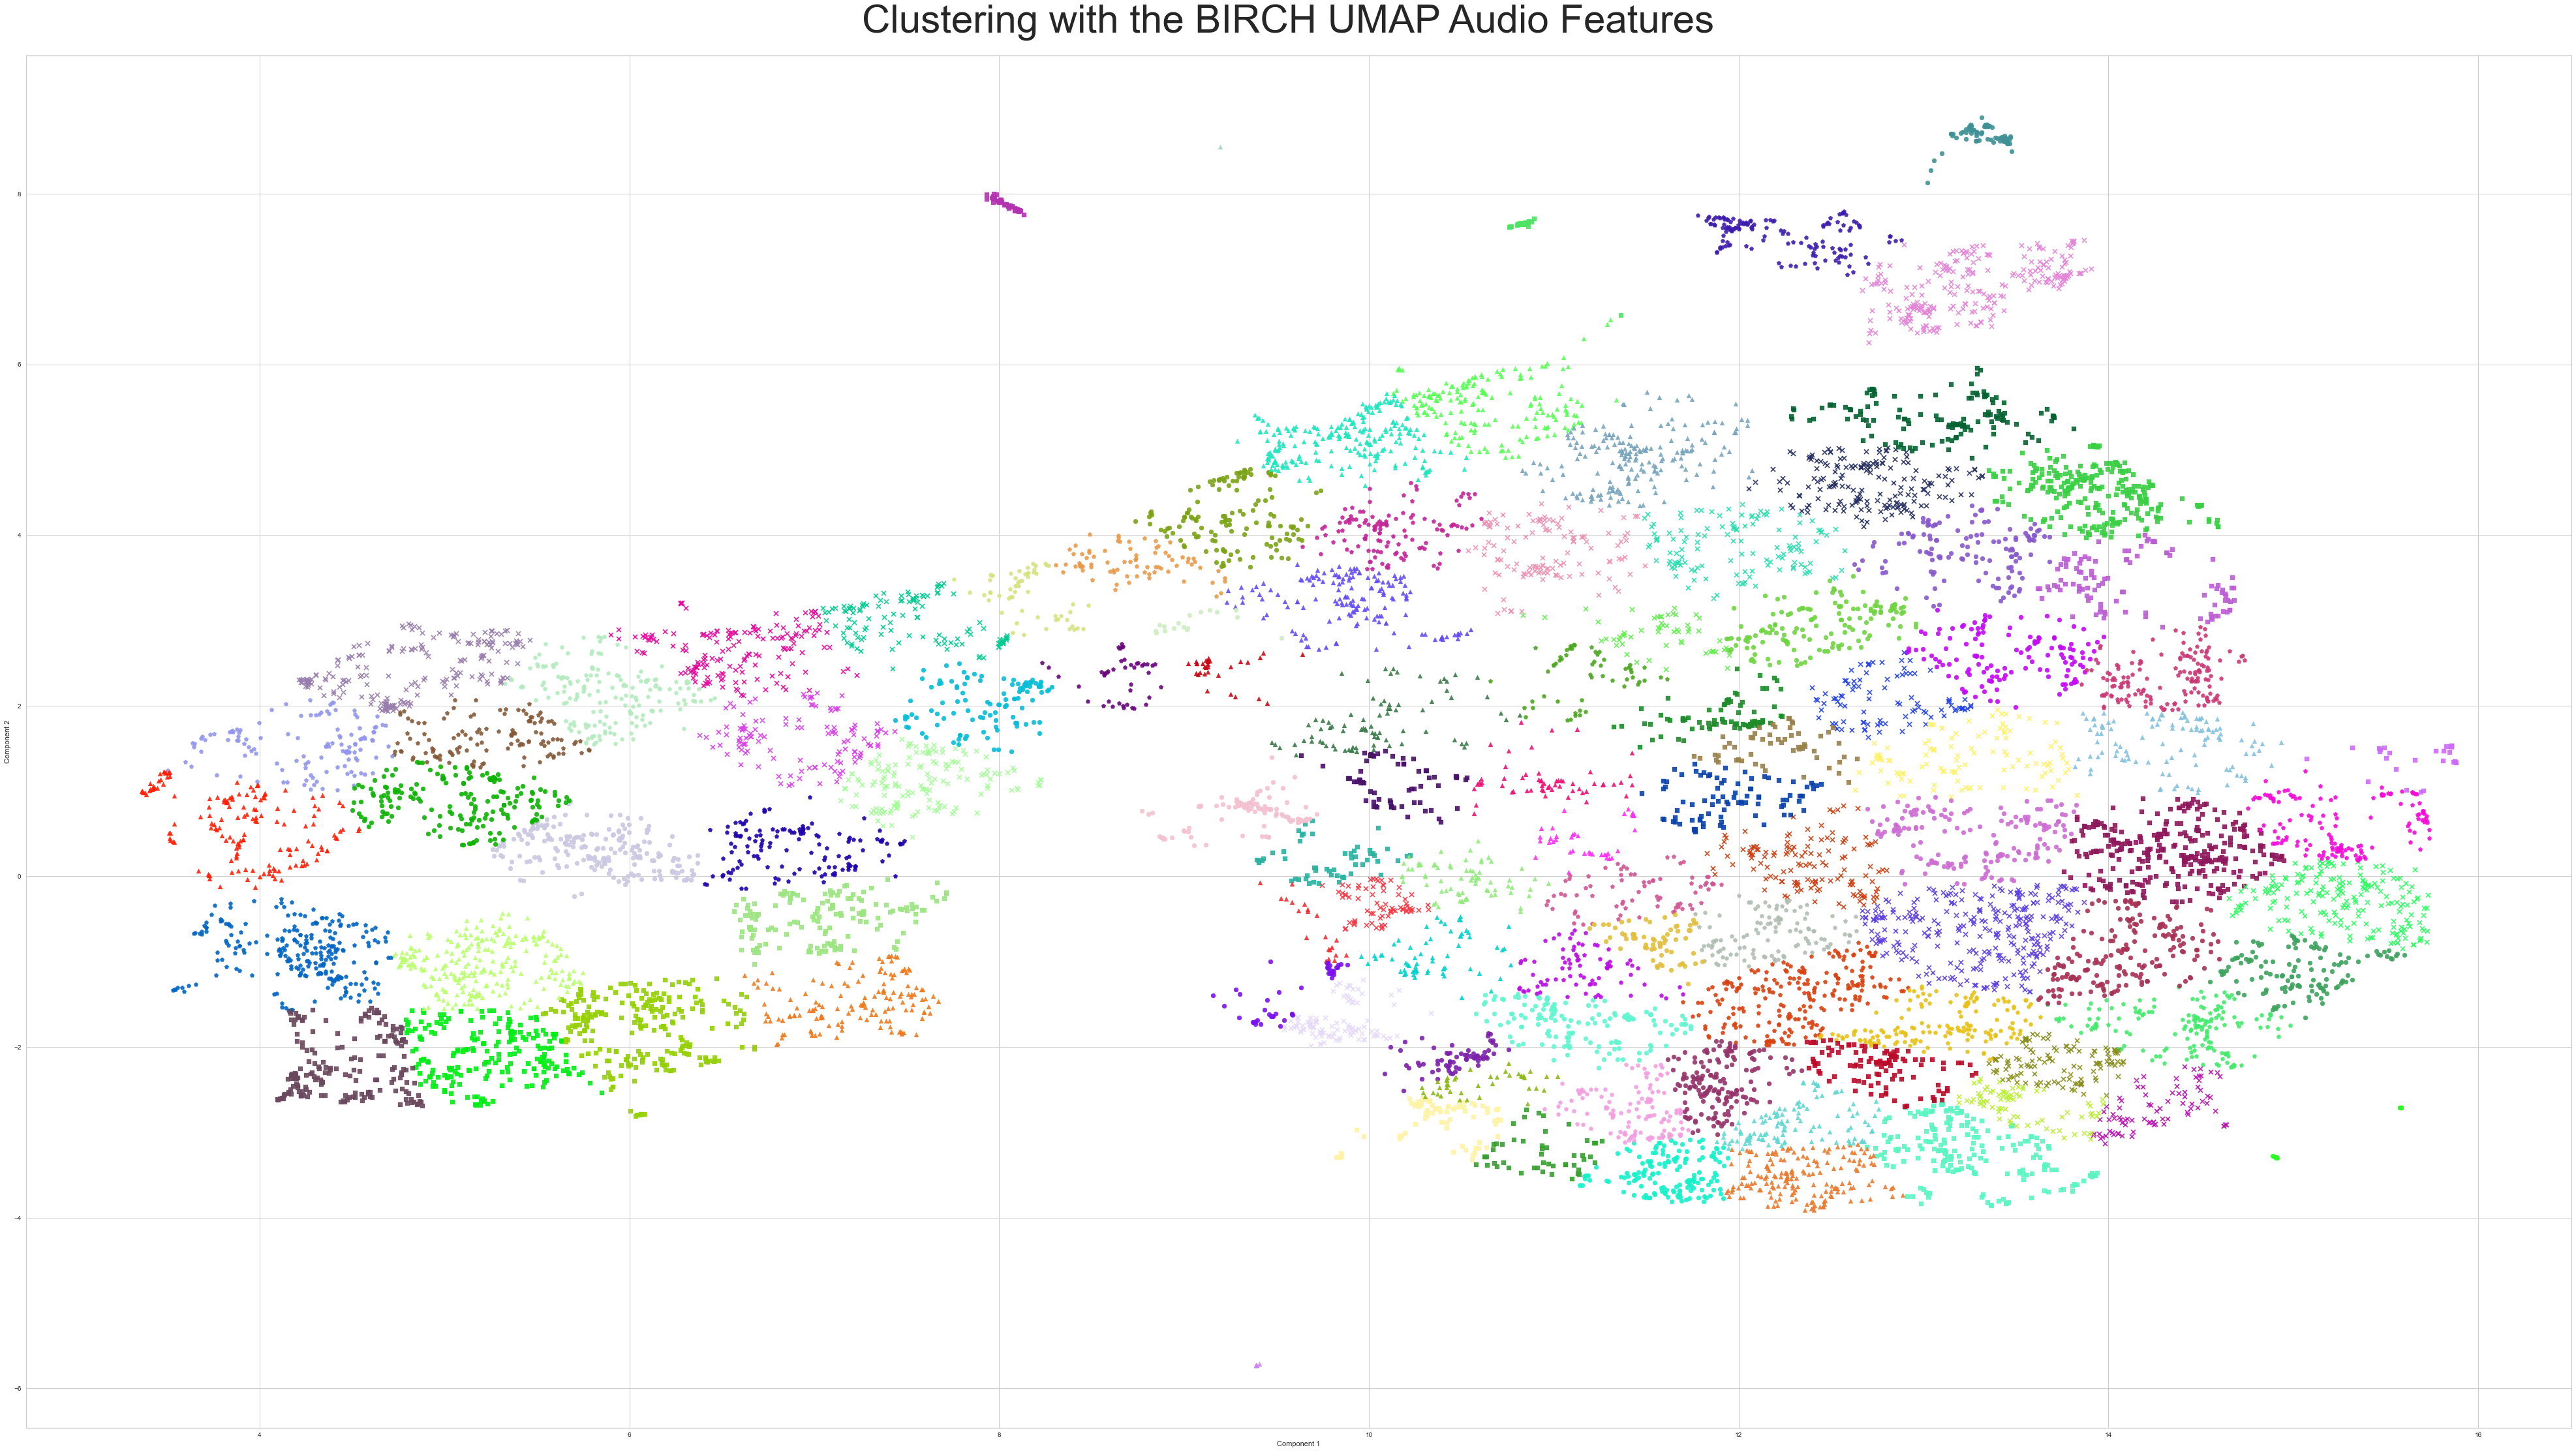
\includegraphics[scale=0.08]{Outputs/BIRCH Clustering - UMAP Audio Features.png}
    \caption{BIRCH clustering on UMAP derived audio features}
    \label{fig:birch-third}
\end{figure}
\begin{figure}[!htb]
    \centering
    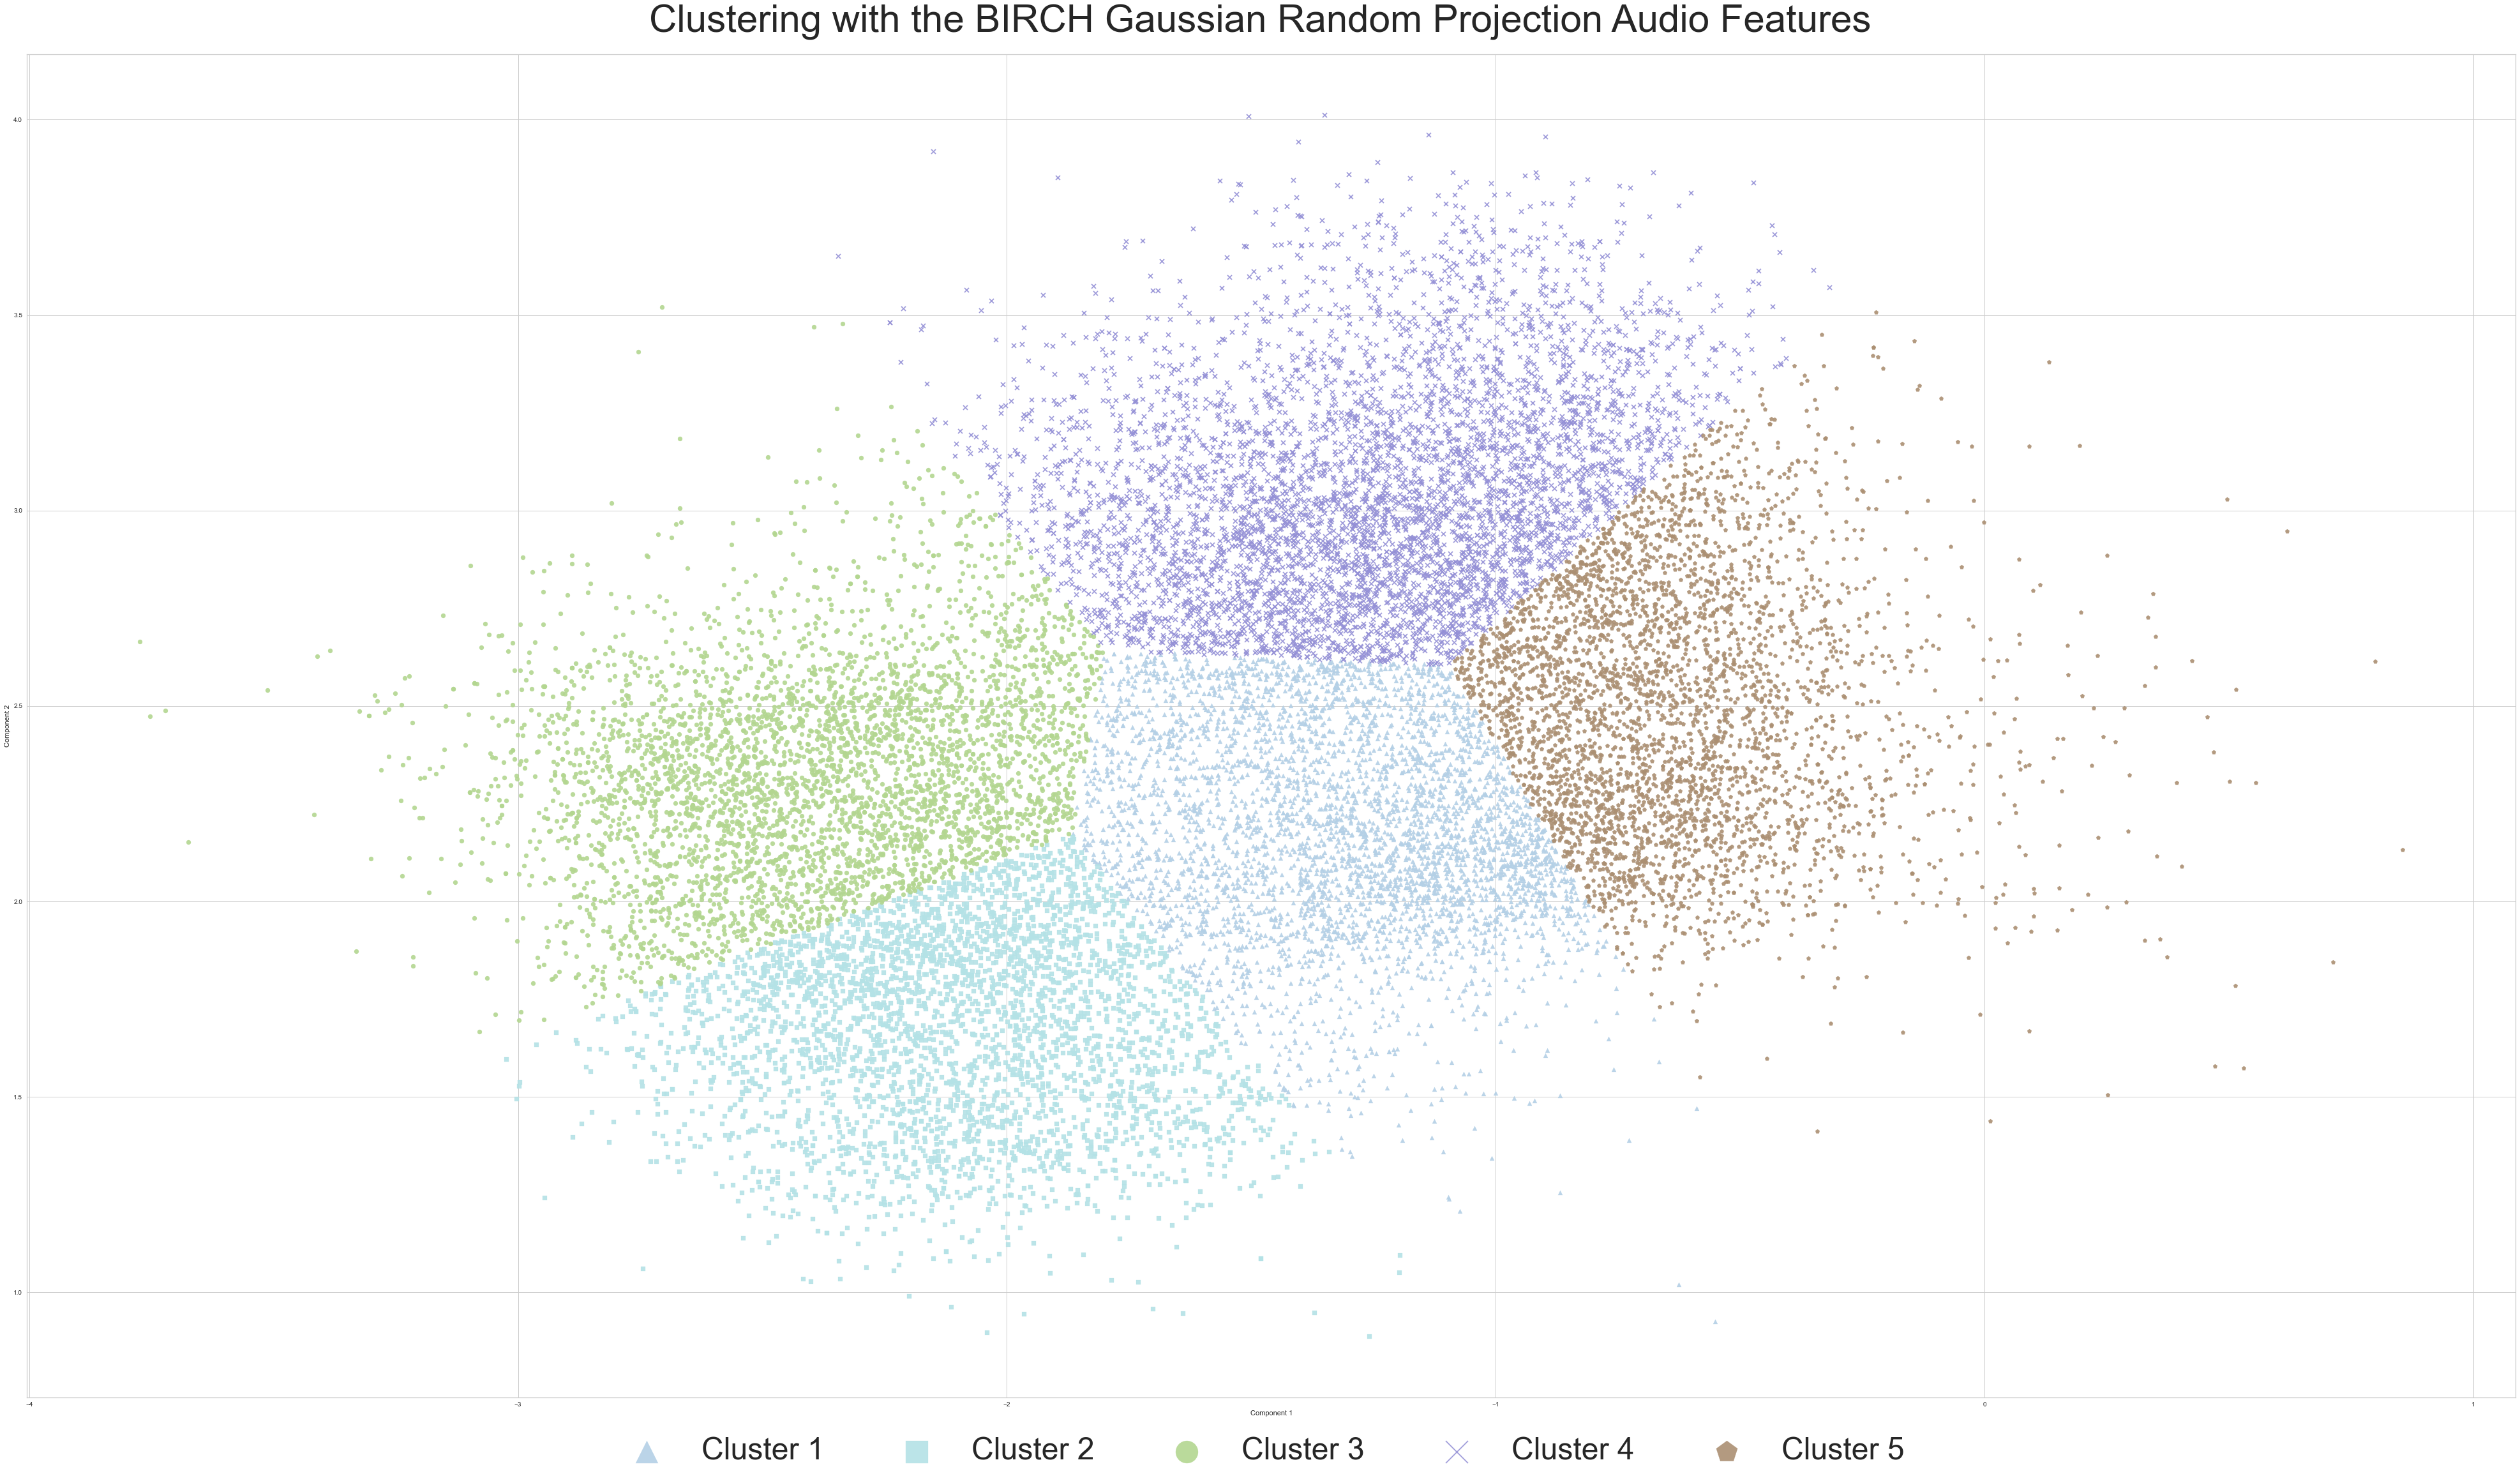
\includegraphics[scale=0.08]{Outputs/BIRCH Clustering - Gaussian Random Projections Audio Features.png}
    \caption{BIRCH clustering on Gaussian Random Projections derived audio features}
    \label{fig:birch-fourth}
\end{figure}
\begin{figure}[htp]
    \centering
    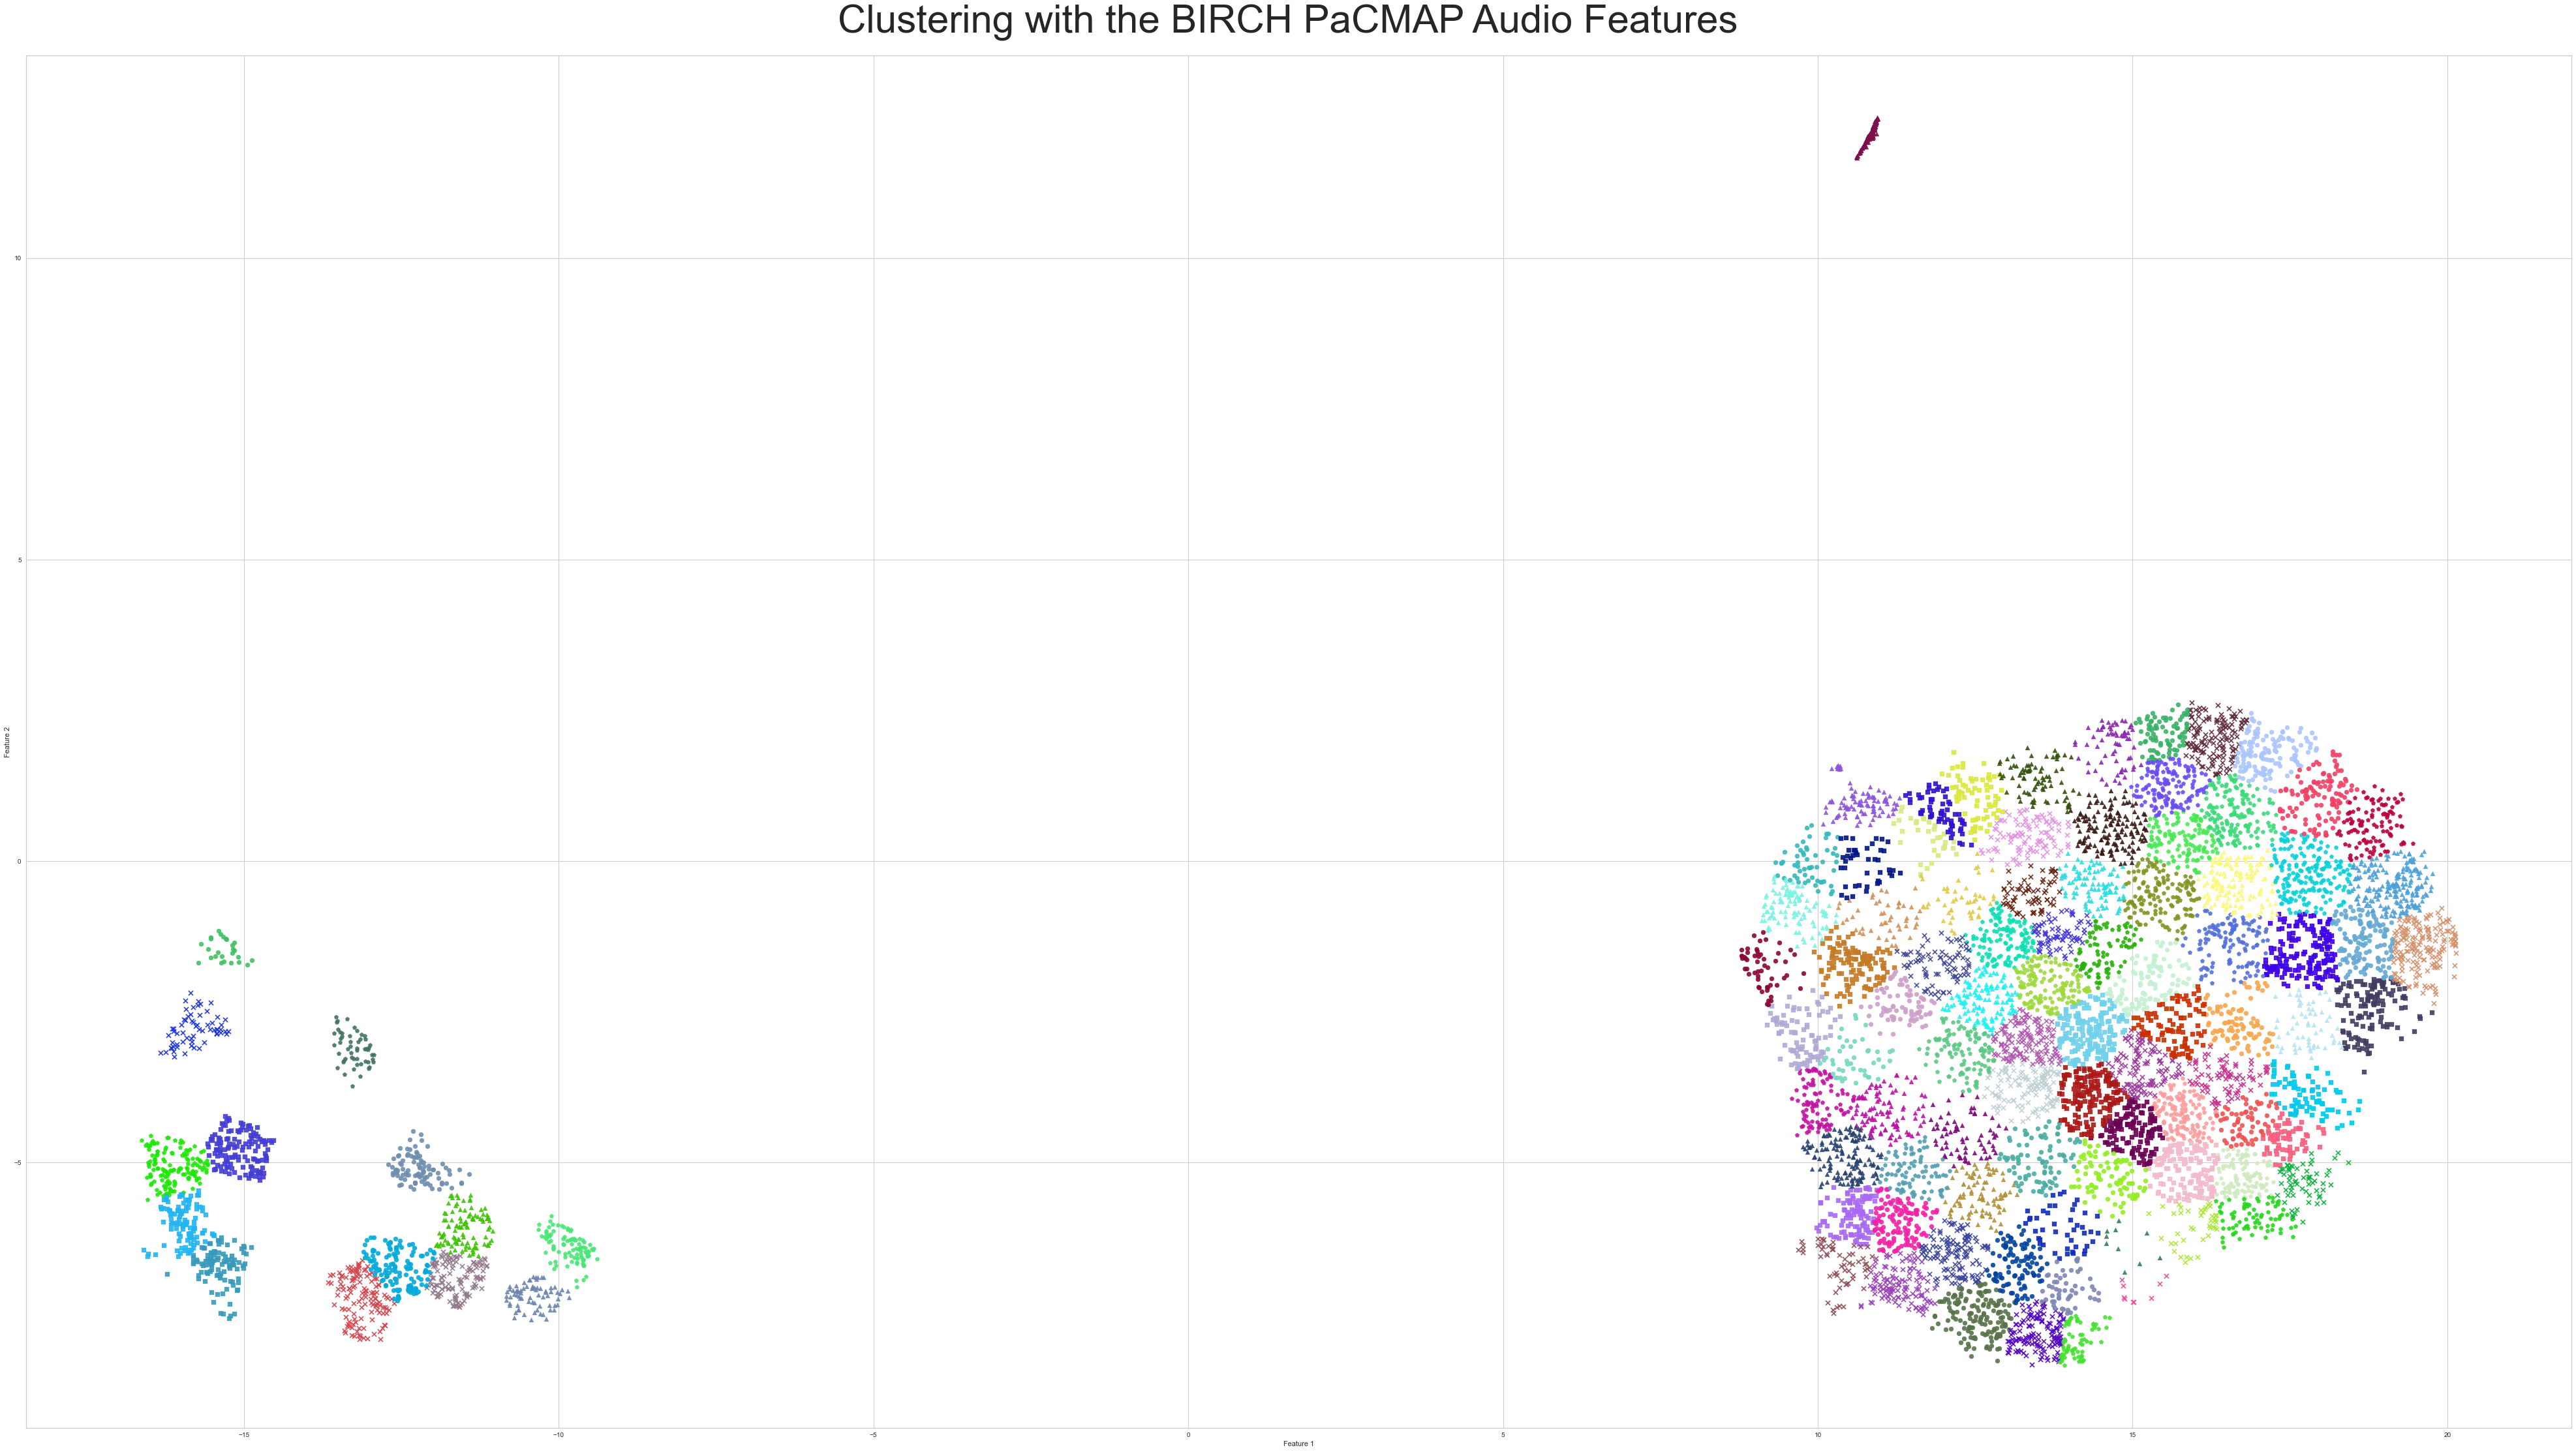
\includegraphics[scale=0.08]{Outputs/BIRCH Clustering - PaCMAP Audio Features.png}
    \caption{BIRCH clustering on the PaCMAP derived audio features}
    \label{fig:birch-fifth}
\end{figure}
\begin{figure}[htp]
    \centering
    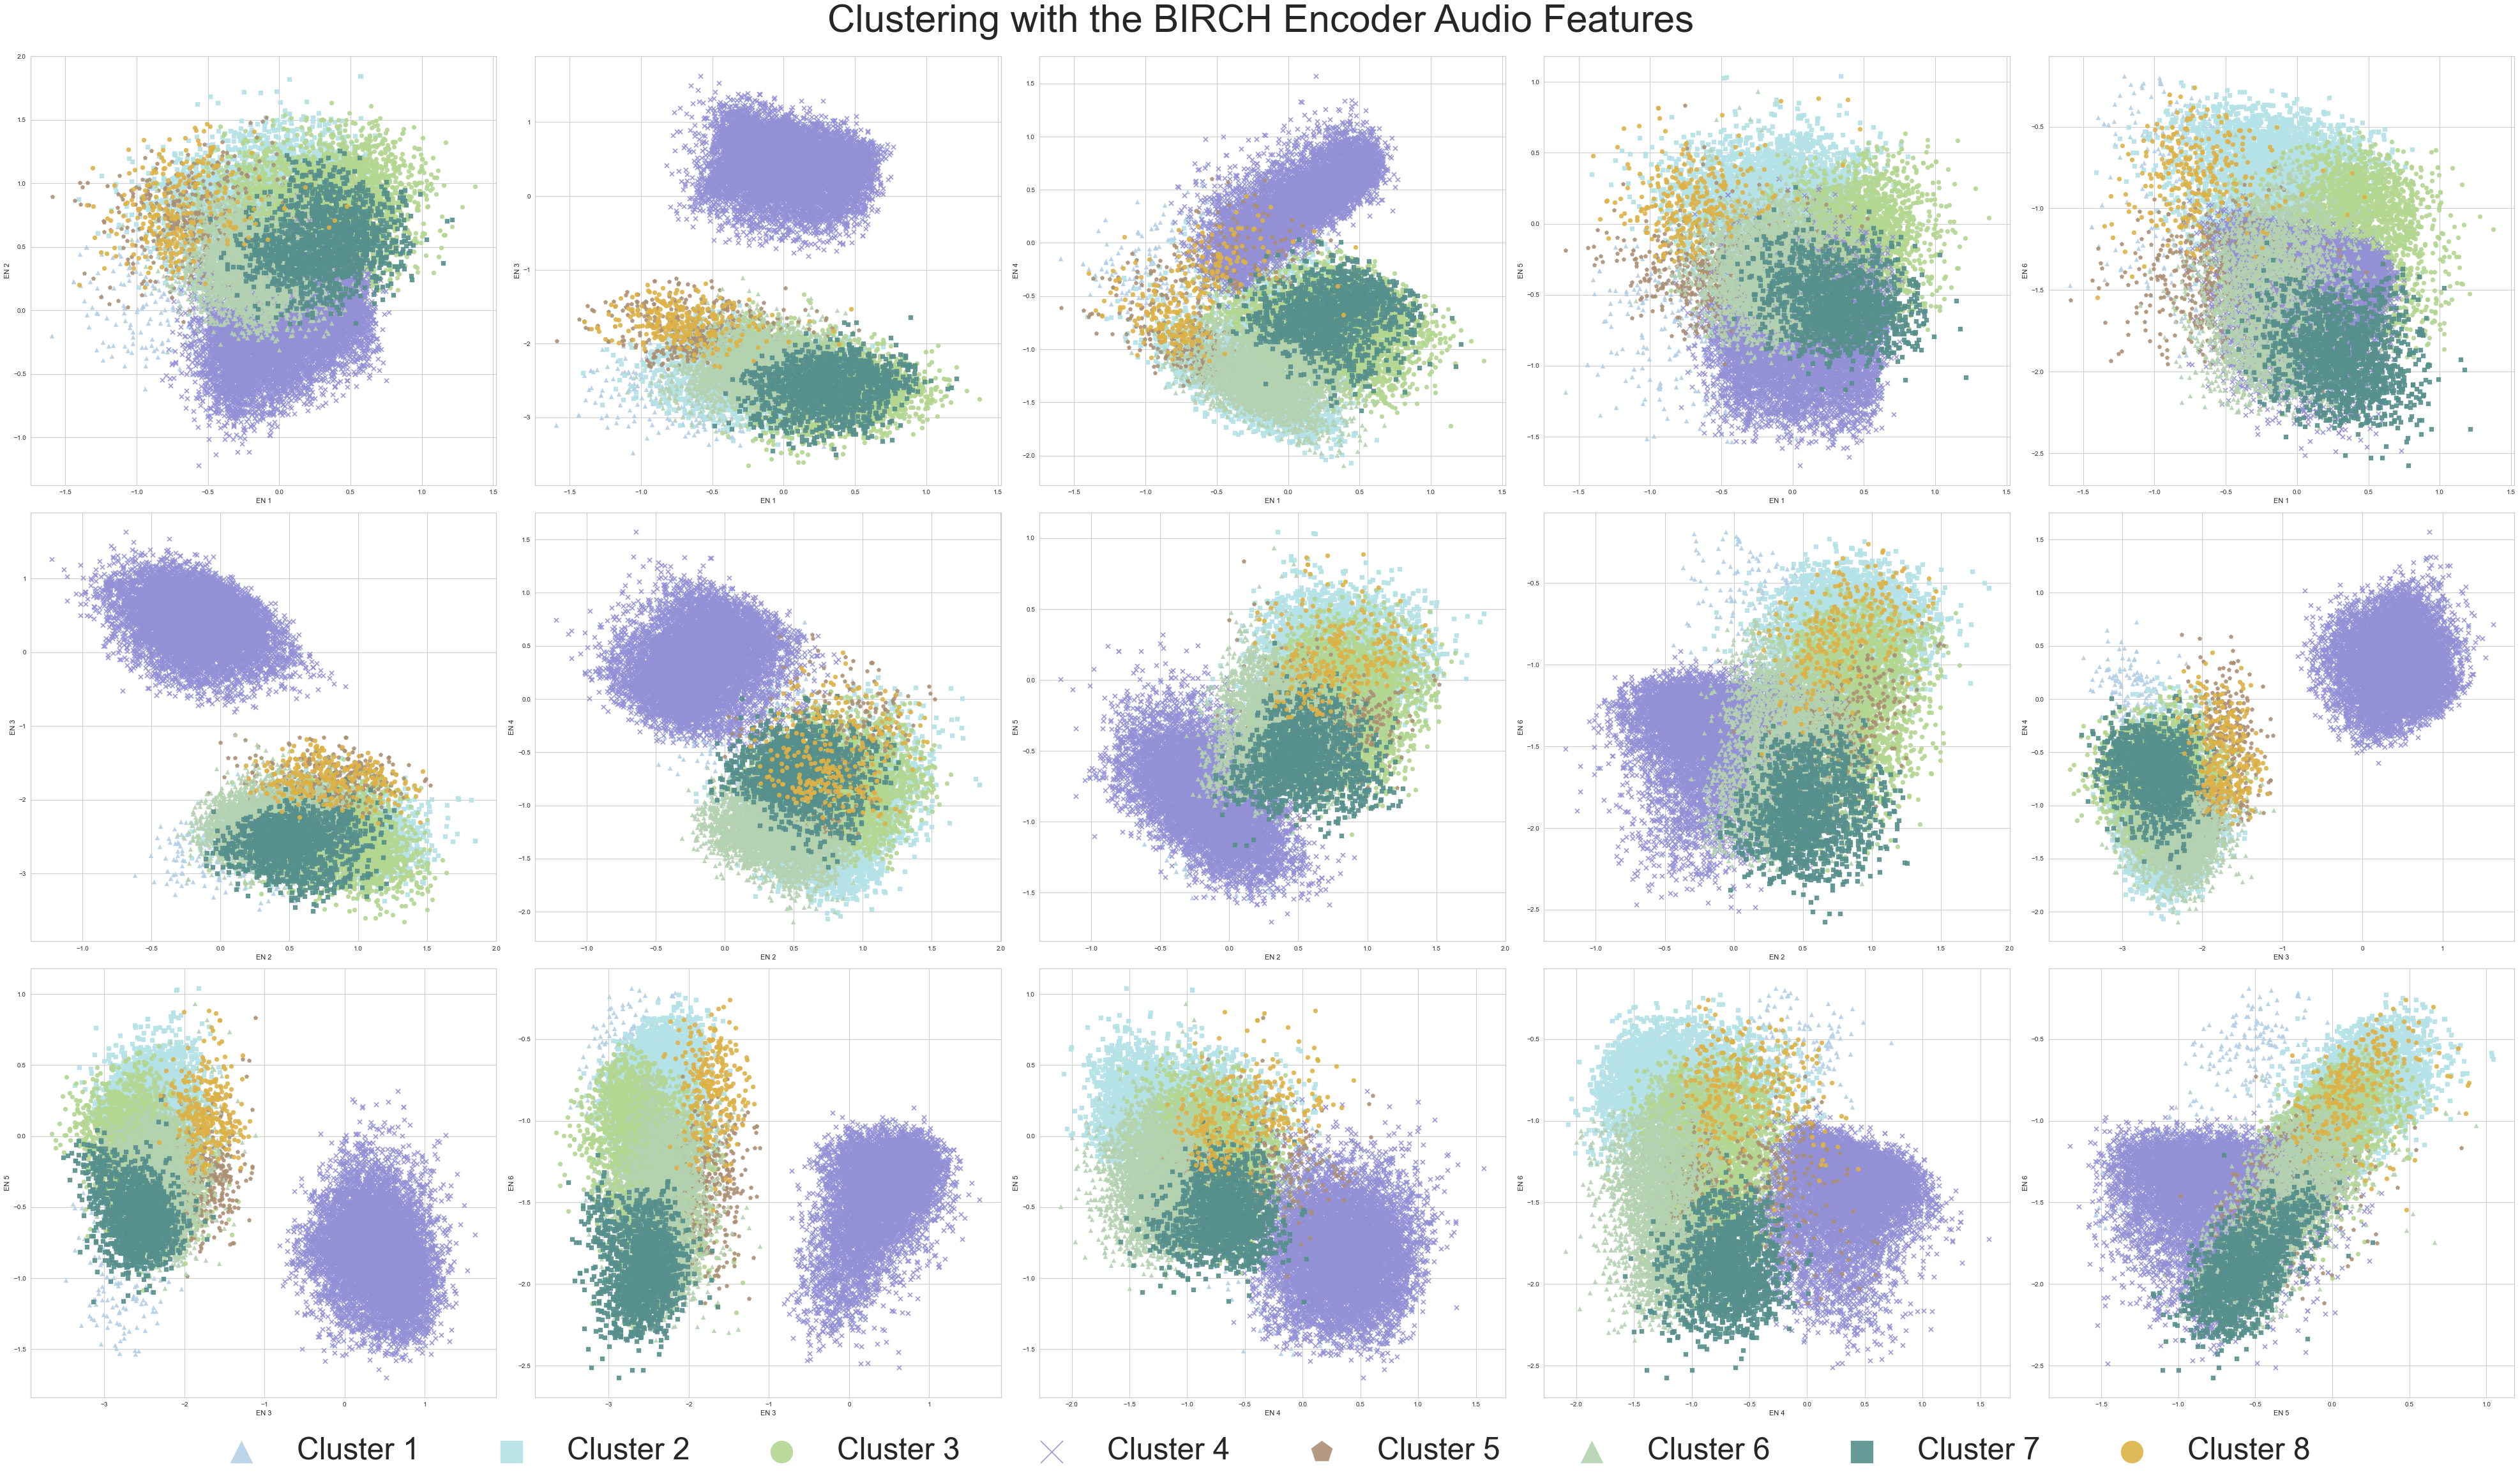
\includegraphics[scale=0.08]{Outputs/BIRCH Clustering - Autoencoder Audio Features.png}
    \caption{BIRCH clustering on the Autoencoder derived audio features}
    \label{fig:birch-sixth}
\end{figure}
\FloatBarrier
\subsection{DBSCAN}
\begin{figure}[htp]
    \centering
    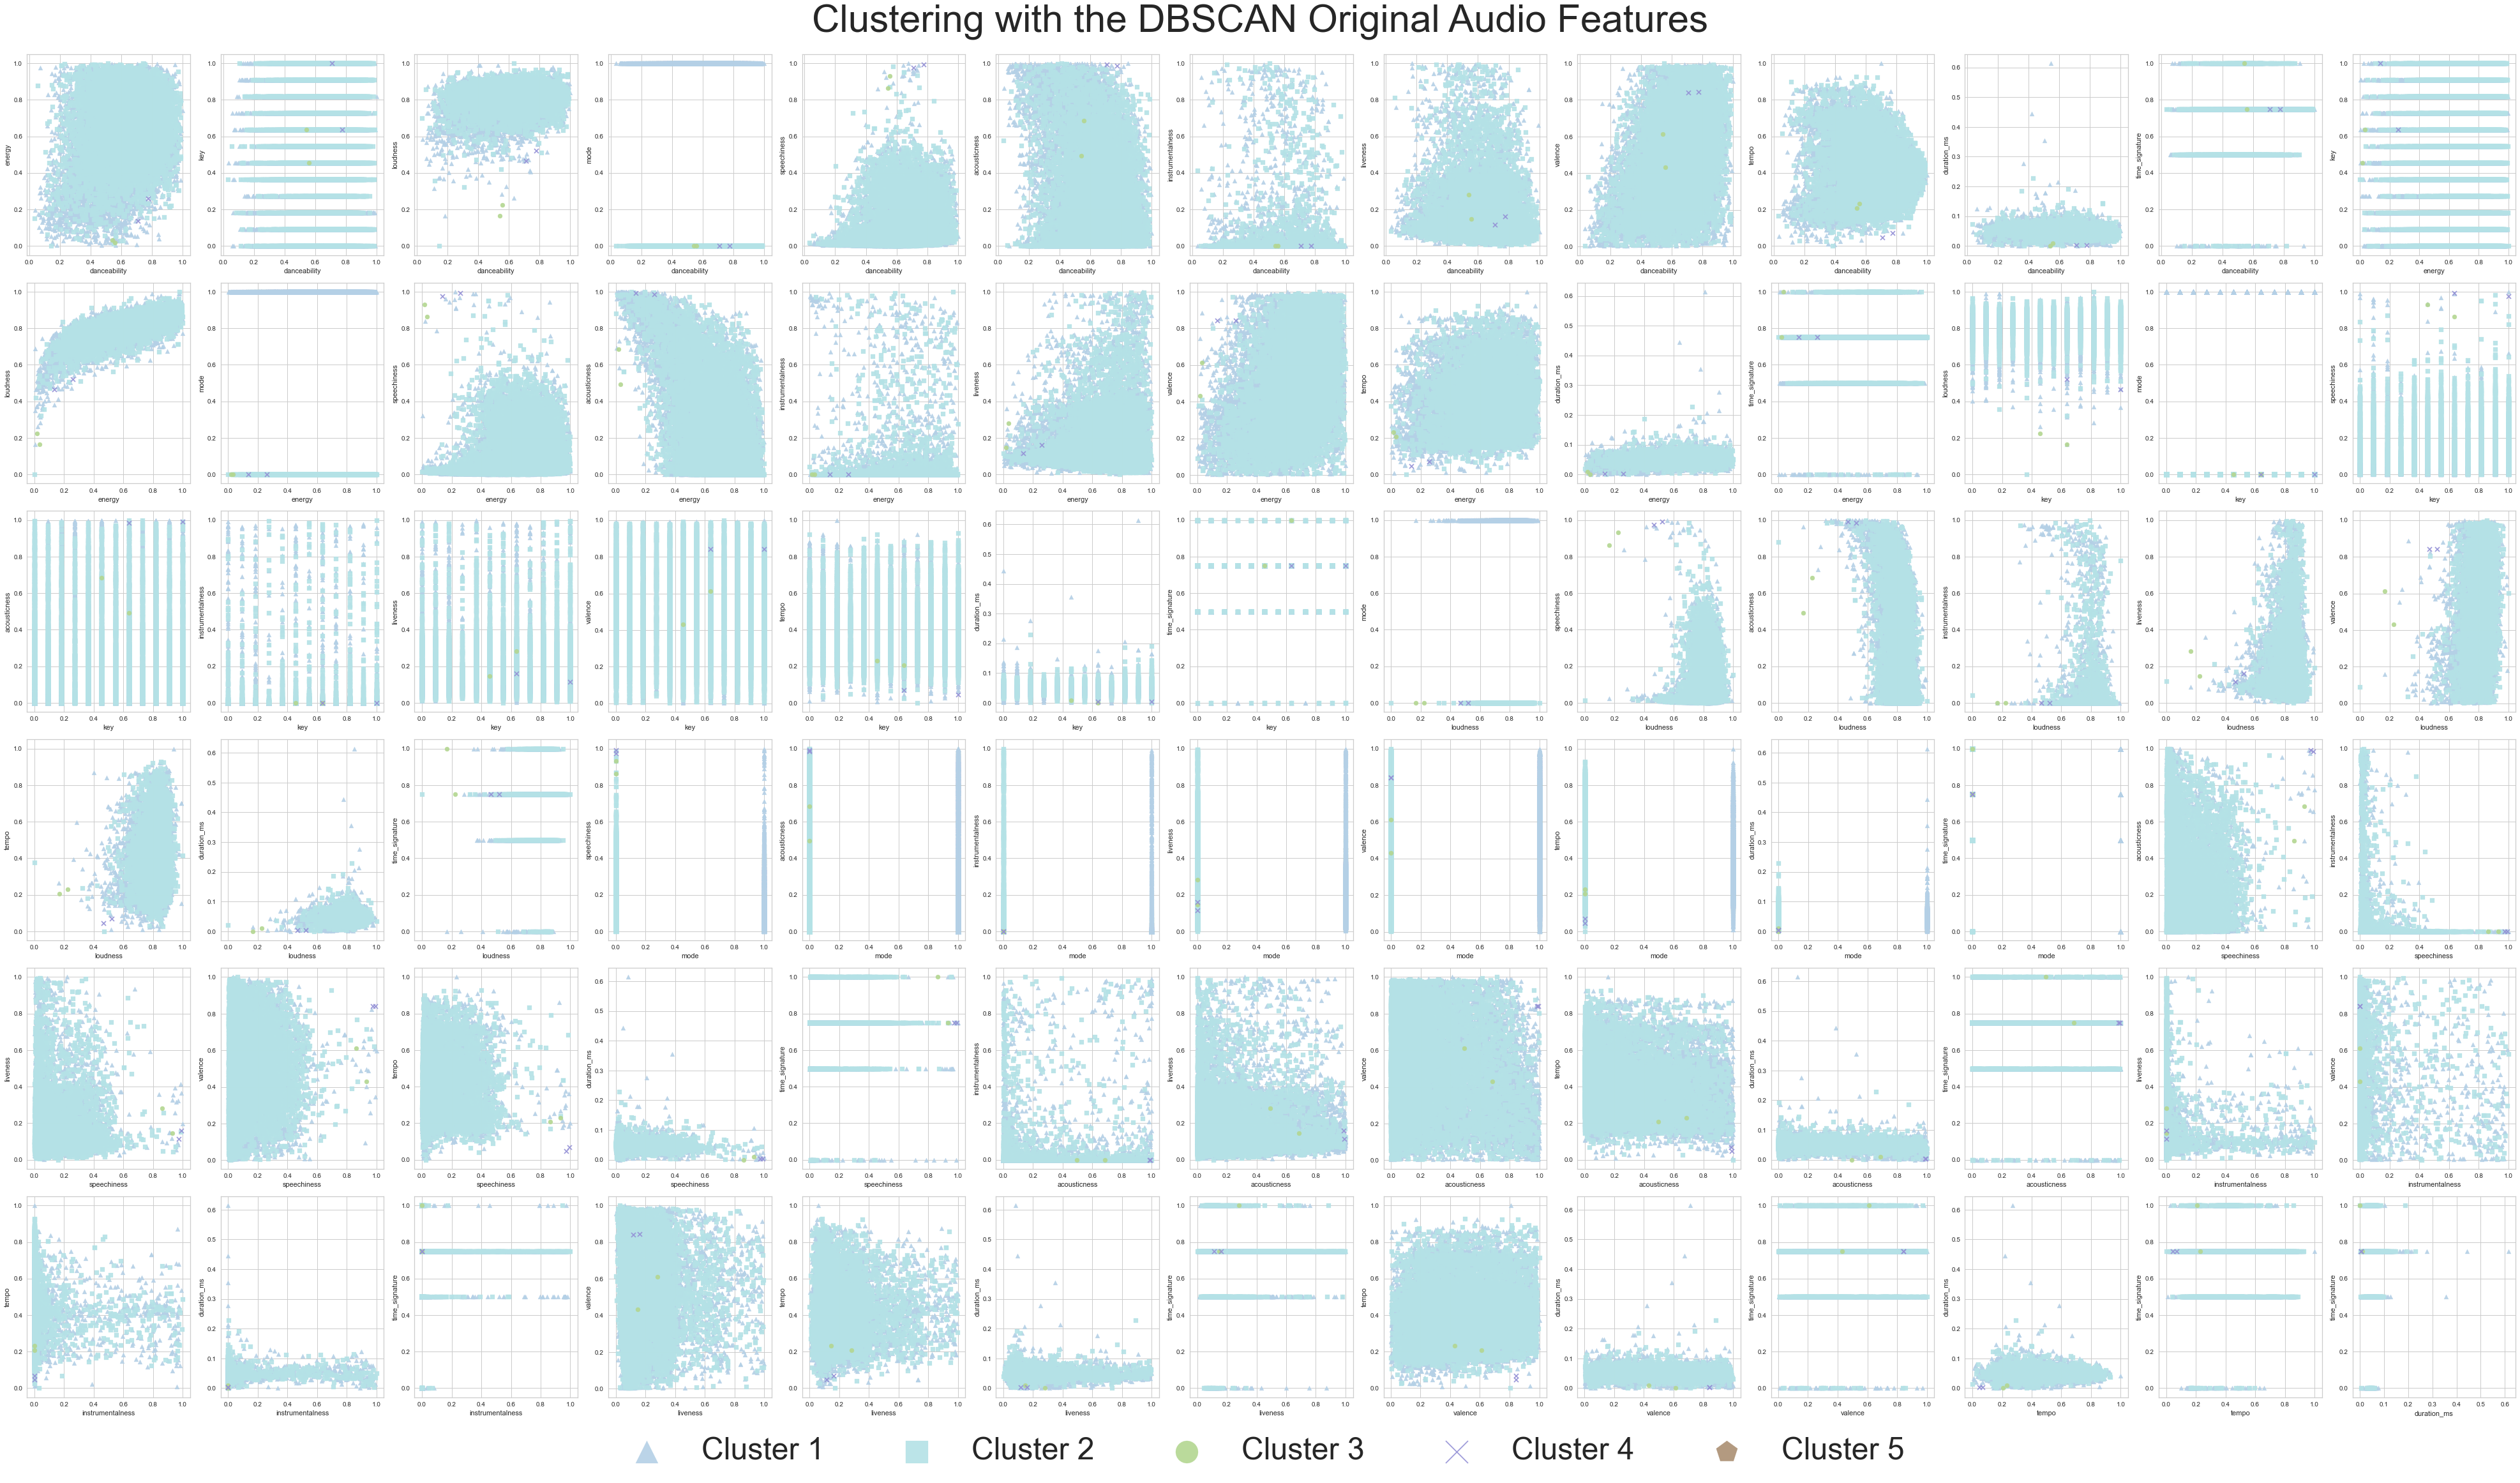
\includegraphics[scale=0.09]{Outputs/DBSCAN Clustering - Original Audio Features.png}
    \caption{DBSCAN clustering on the scaled original audio features}
    \label{fig:dbscan-first}
\end{figure}
\begin{figure}[!htb]
    \centering
    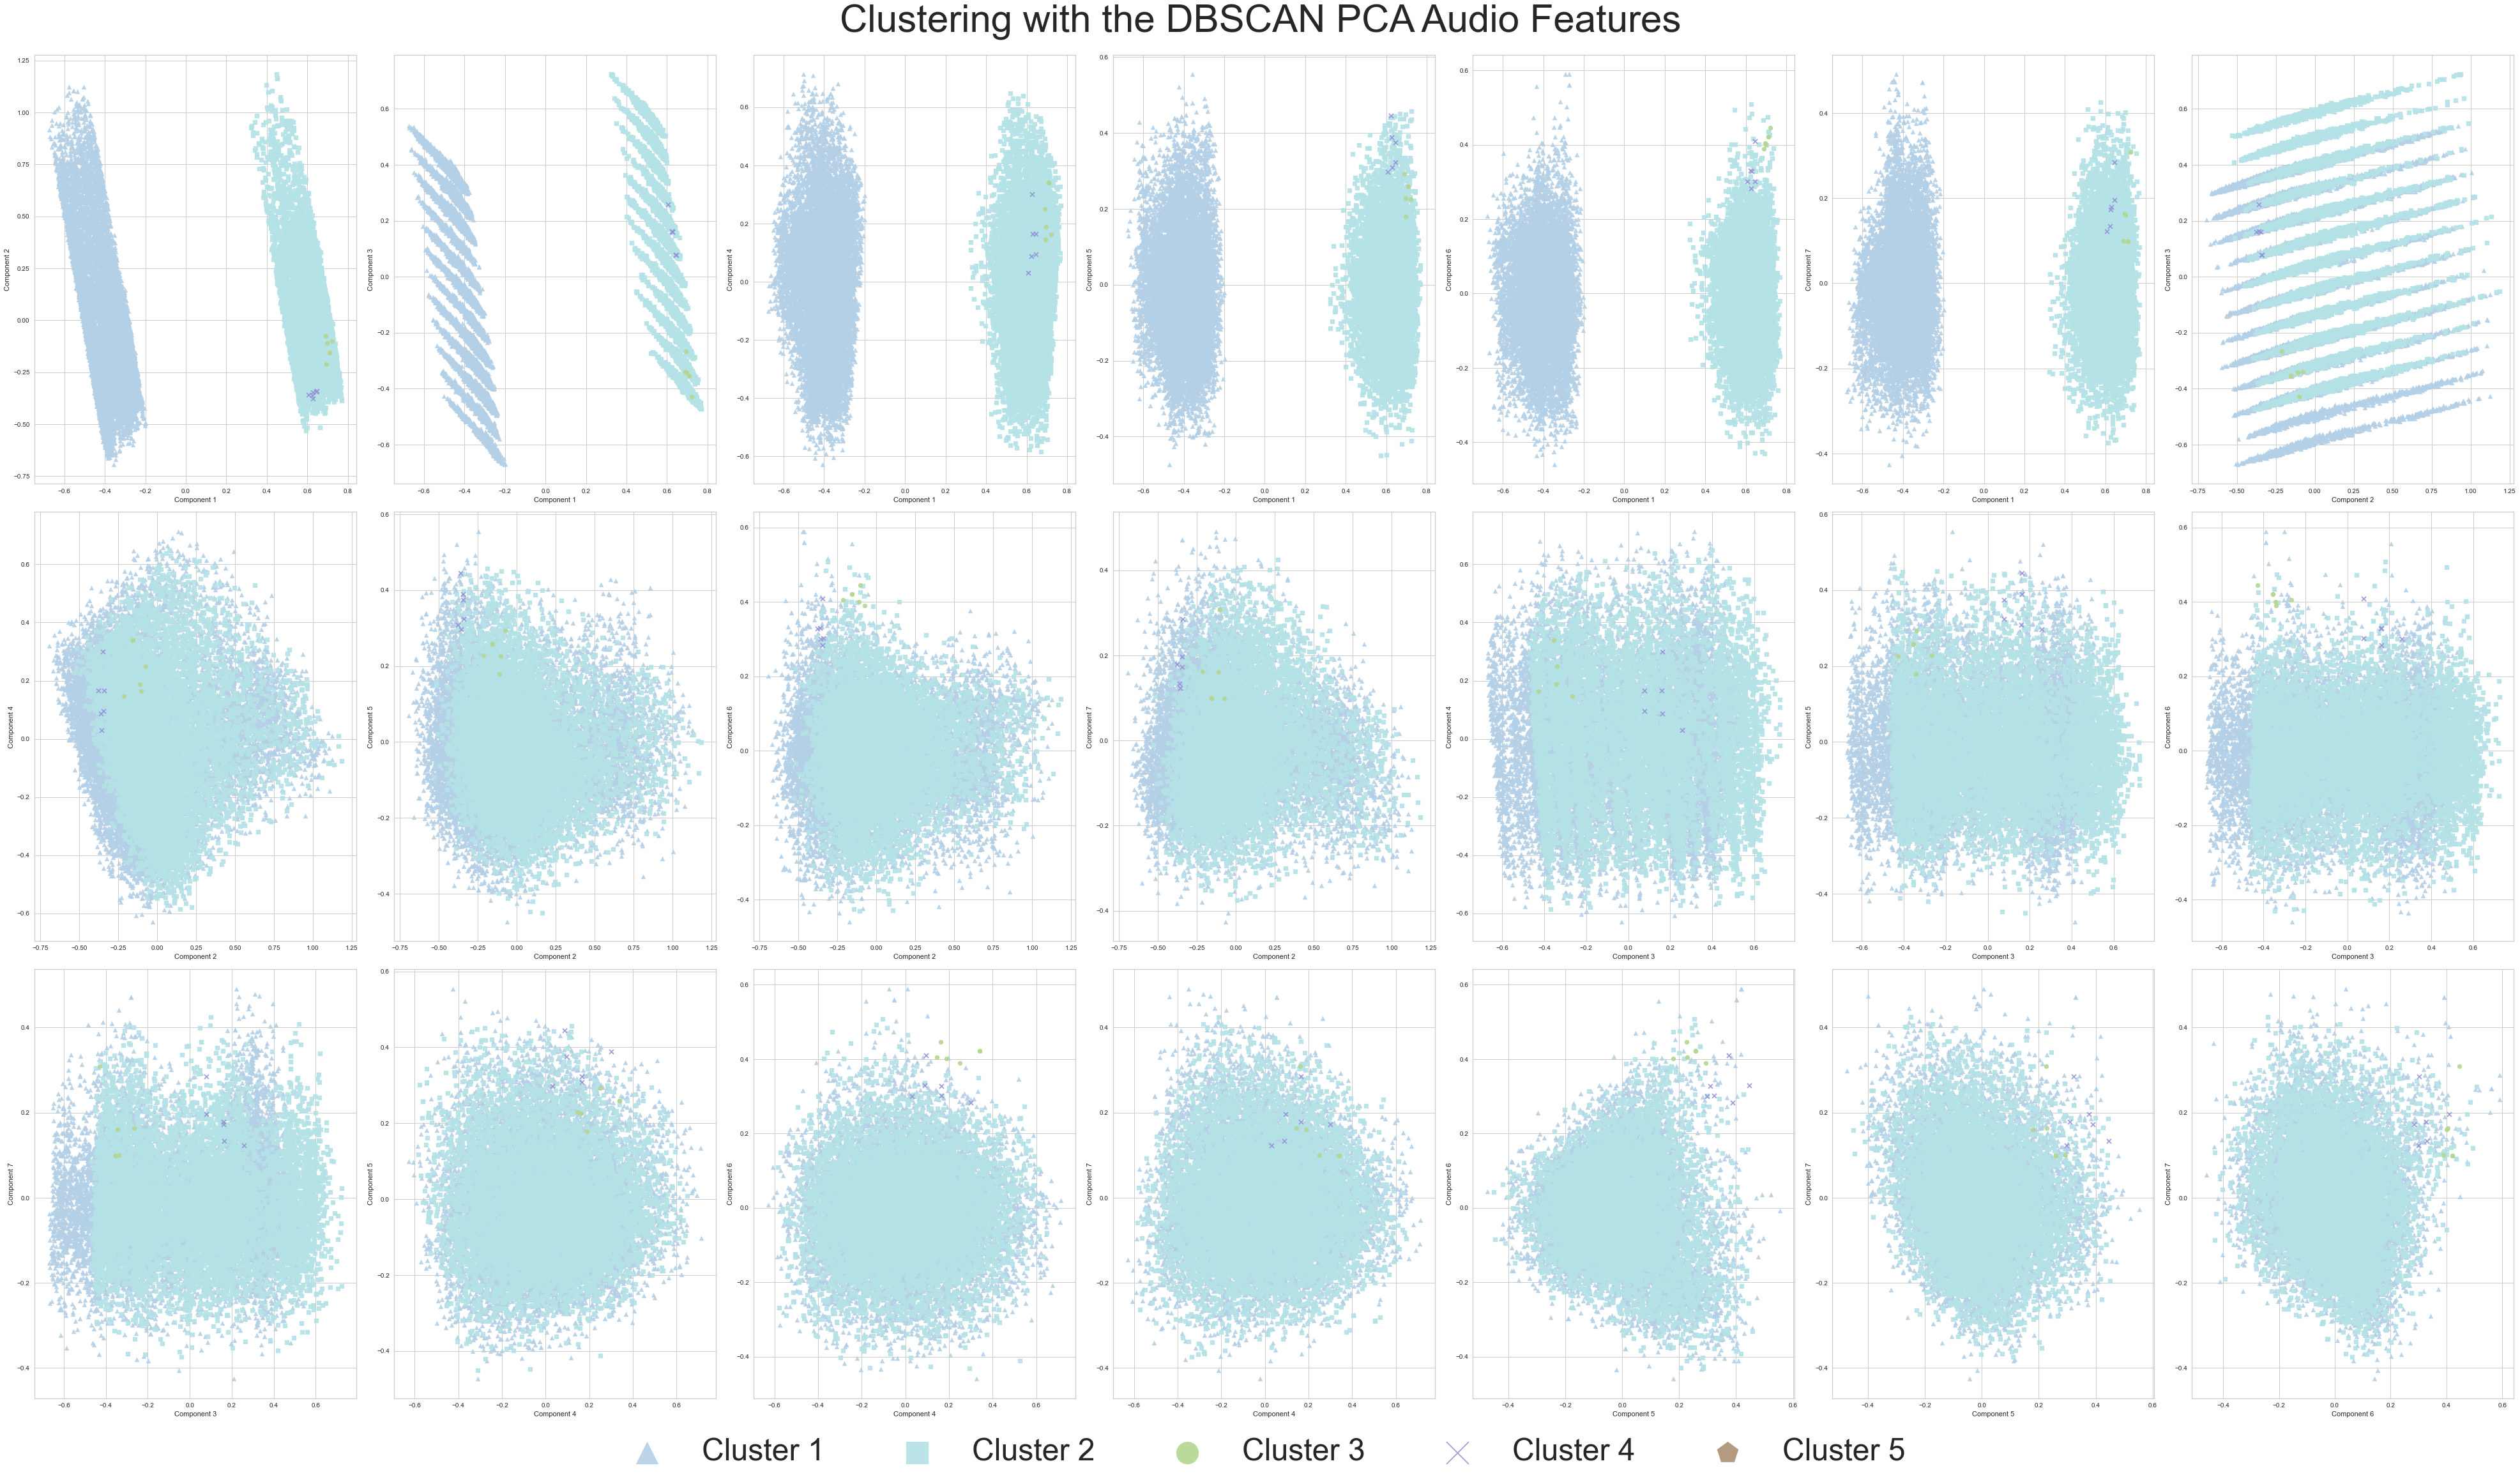
\includegraphics[scale=0.09]{Outputs/DBSCAN Clustering - PCA Audio Features.png}
    \caption{DBSCAN clustering on PCA dervived audio features}
    \label{fig:dbscan-second}
\end{figure}
\begin{figure}
    \centering
    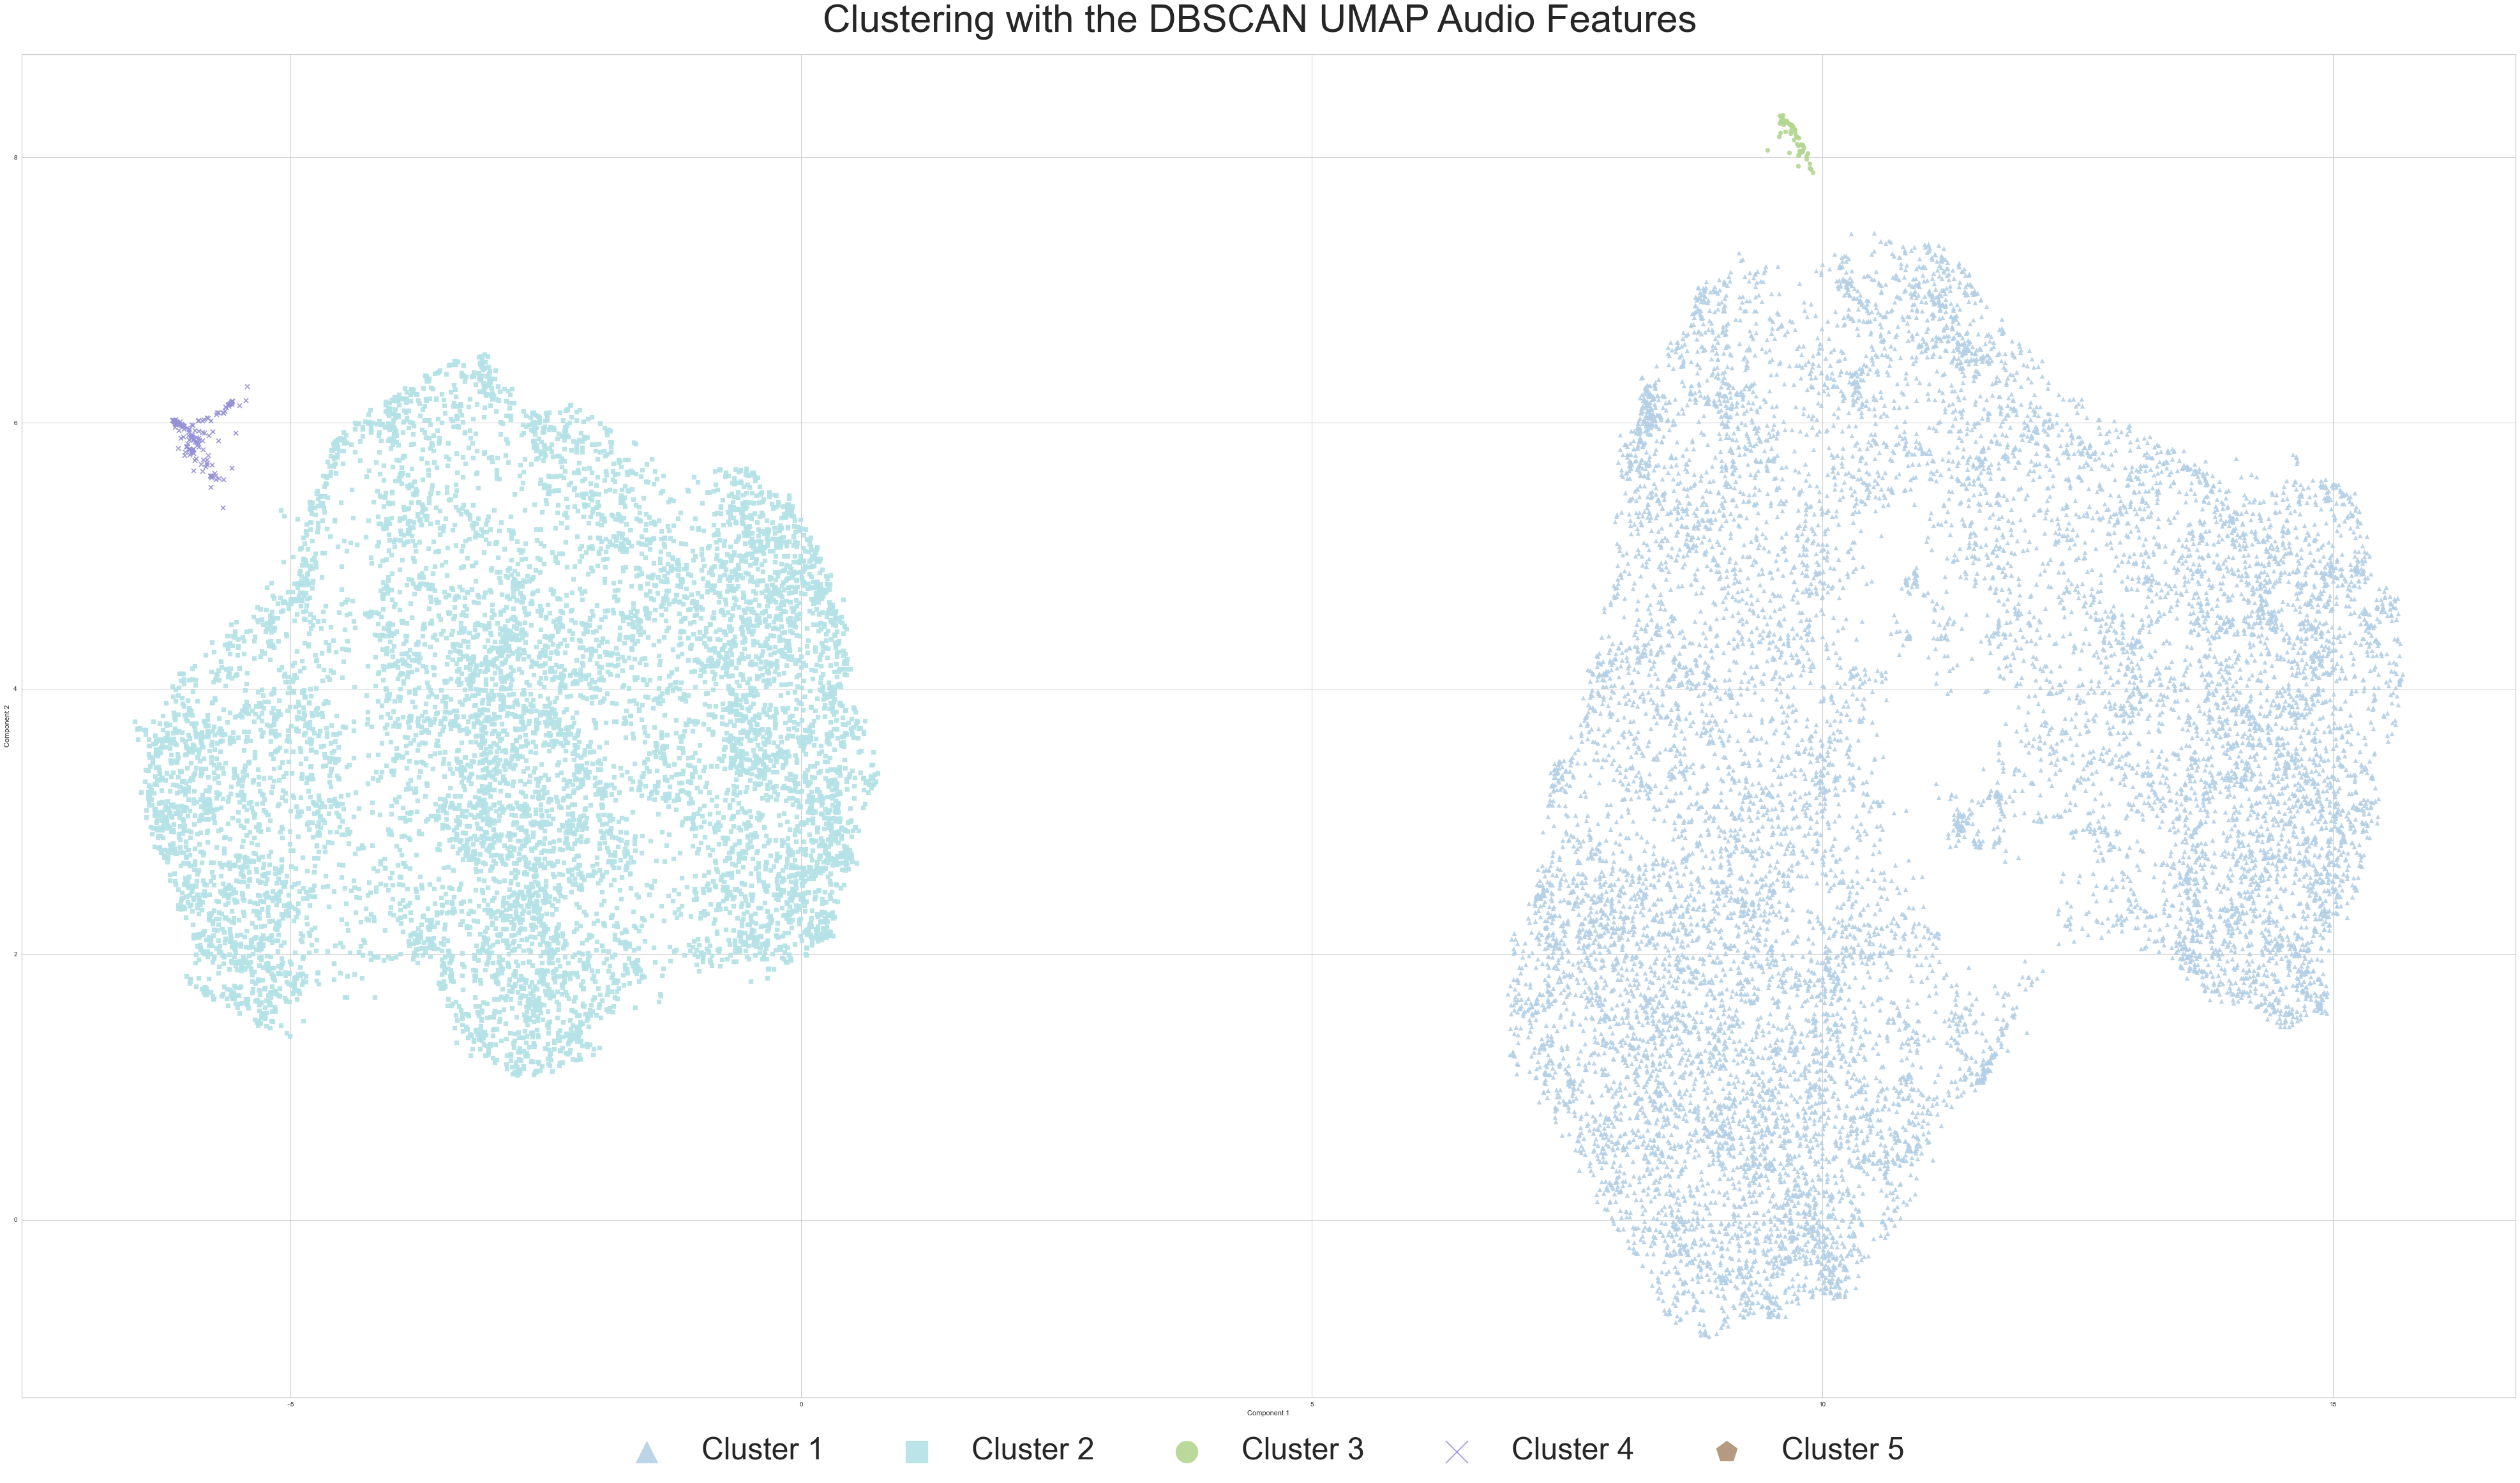
\includegraphics[scale=0.08]{Outputs/DBSCAN Clustering - UMAP Audio Features.png}
    \caption{DBSCAN clustering on UMAP derived audio features}
    \label{fig:dbscan-third}
\end{figure}
\begin{figure}
    \centering
    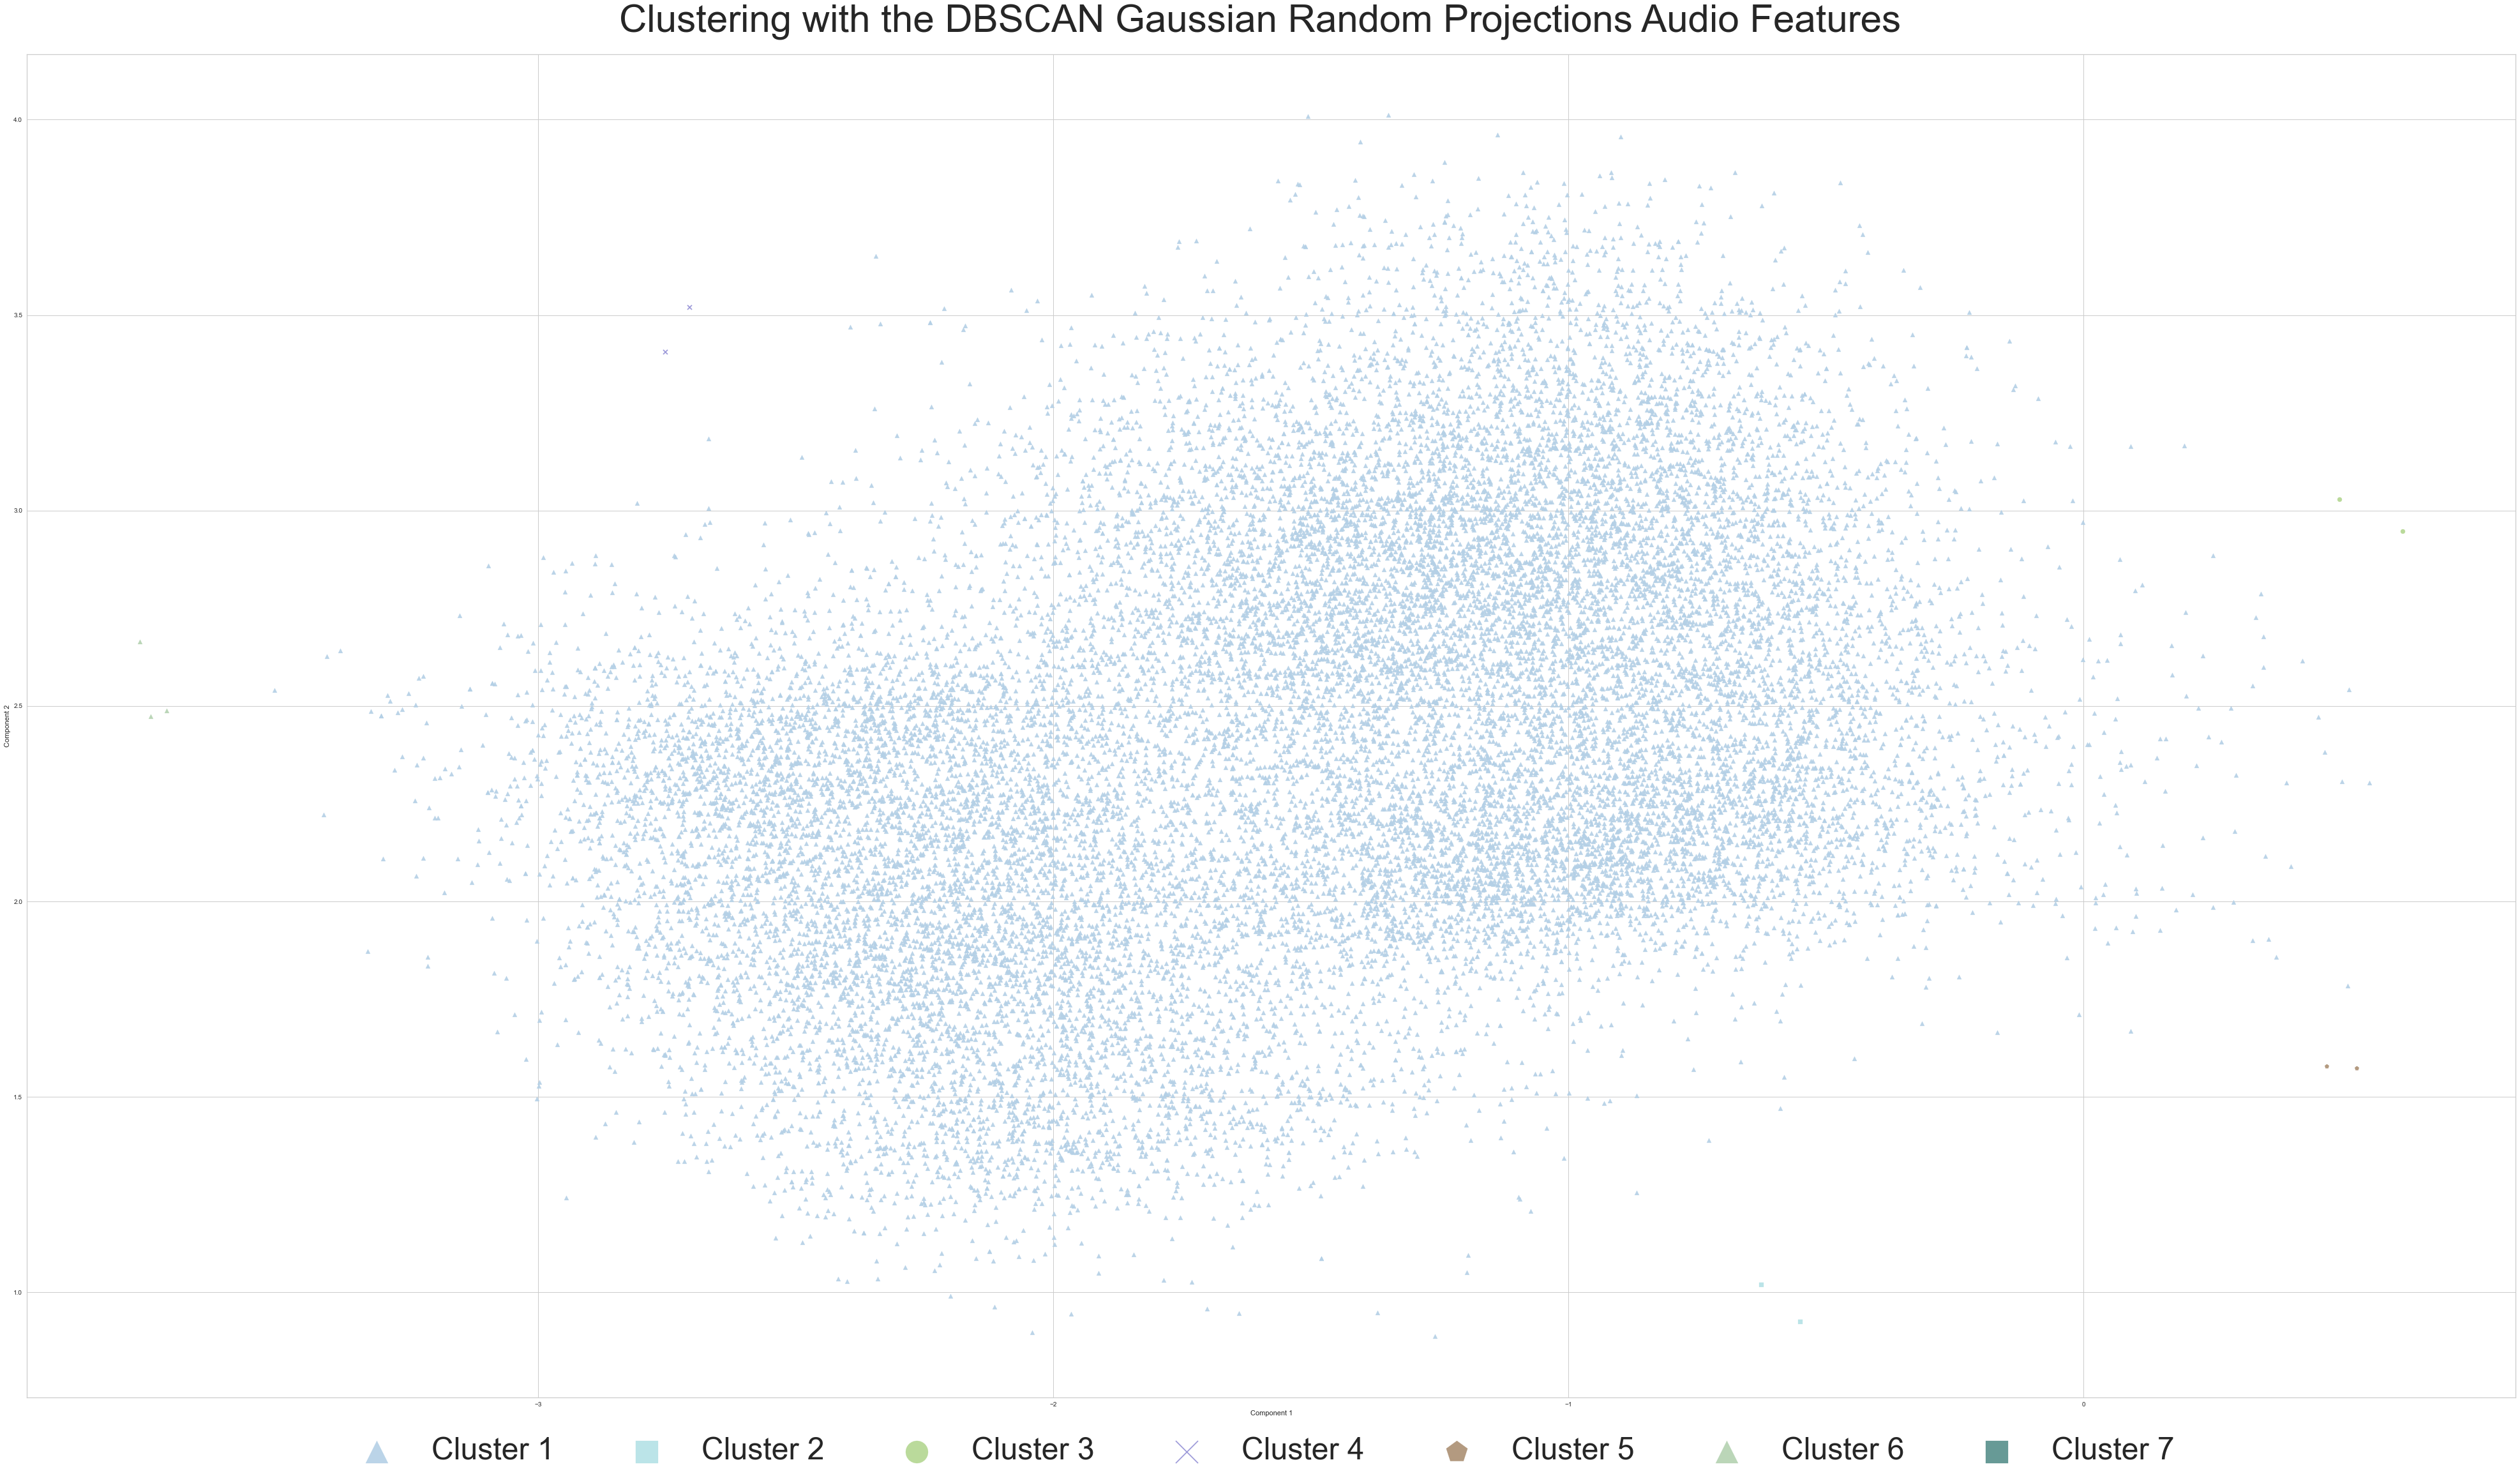
\includegraphics[scale=0.08]{Outputs/DBSCAN Clustering - Gaussian Random Projections Audio Features.png}
    \caption{DBSCAN clustering on Gaussian Random Projections derived audio features}
    \label{fig:dbscan-fourth}
\end{figure}
\begin{figure}
    \centering
    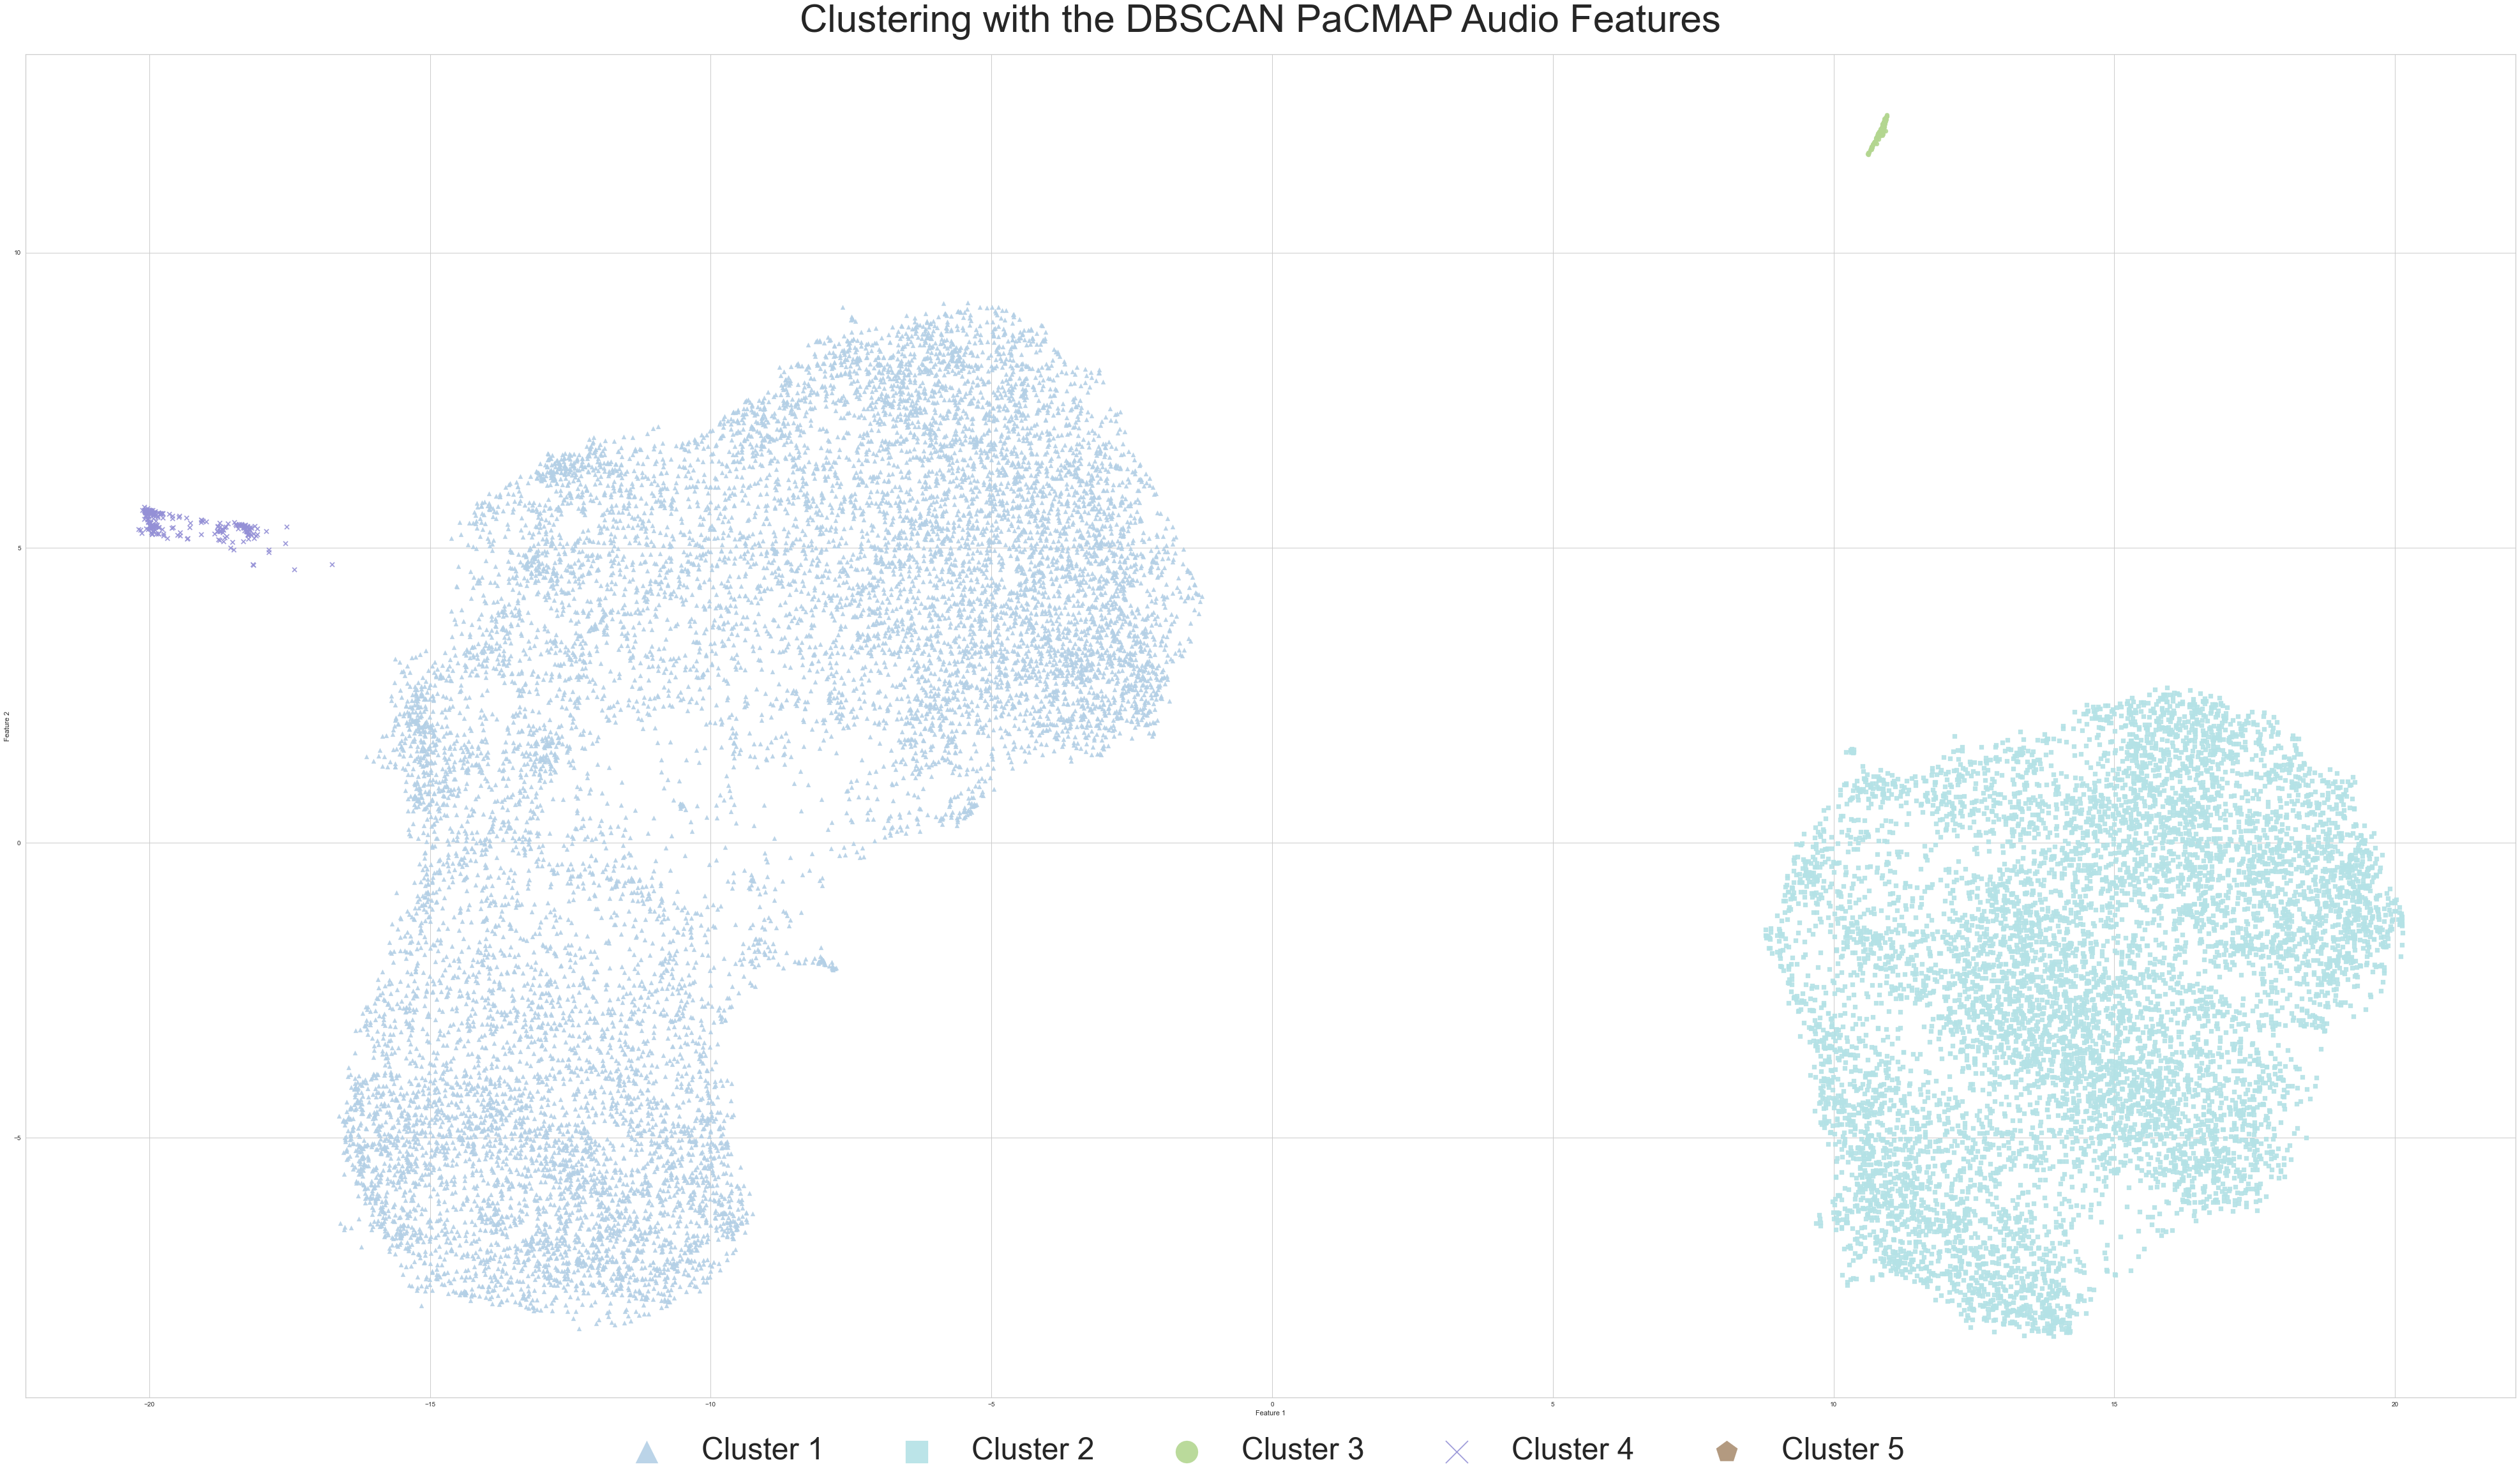
\includegraphics[scale=0.09]{Outputs/DBSCAN Clustering - PaCMAP Audio Features.png}
    \caption{DBSCAN clustering on the PaCMAP derived audio features}
    \label{fig:dbscan-fifth}
\end{figure}
\begin{figure}
    \centering
    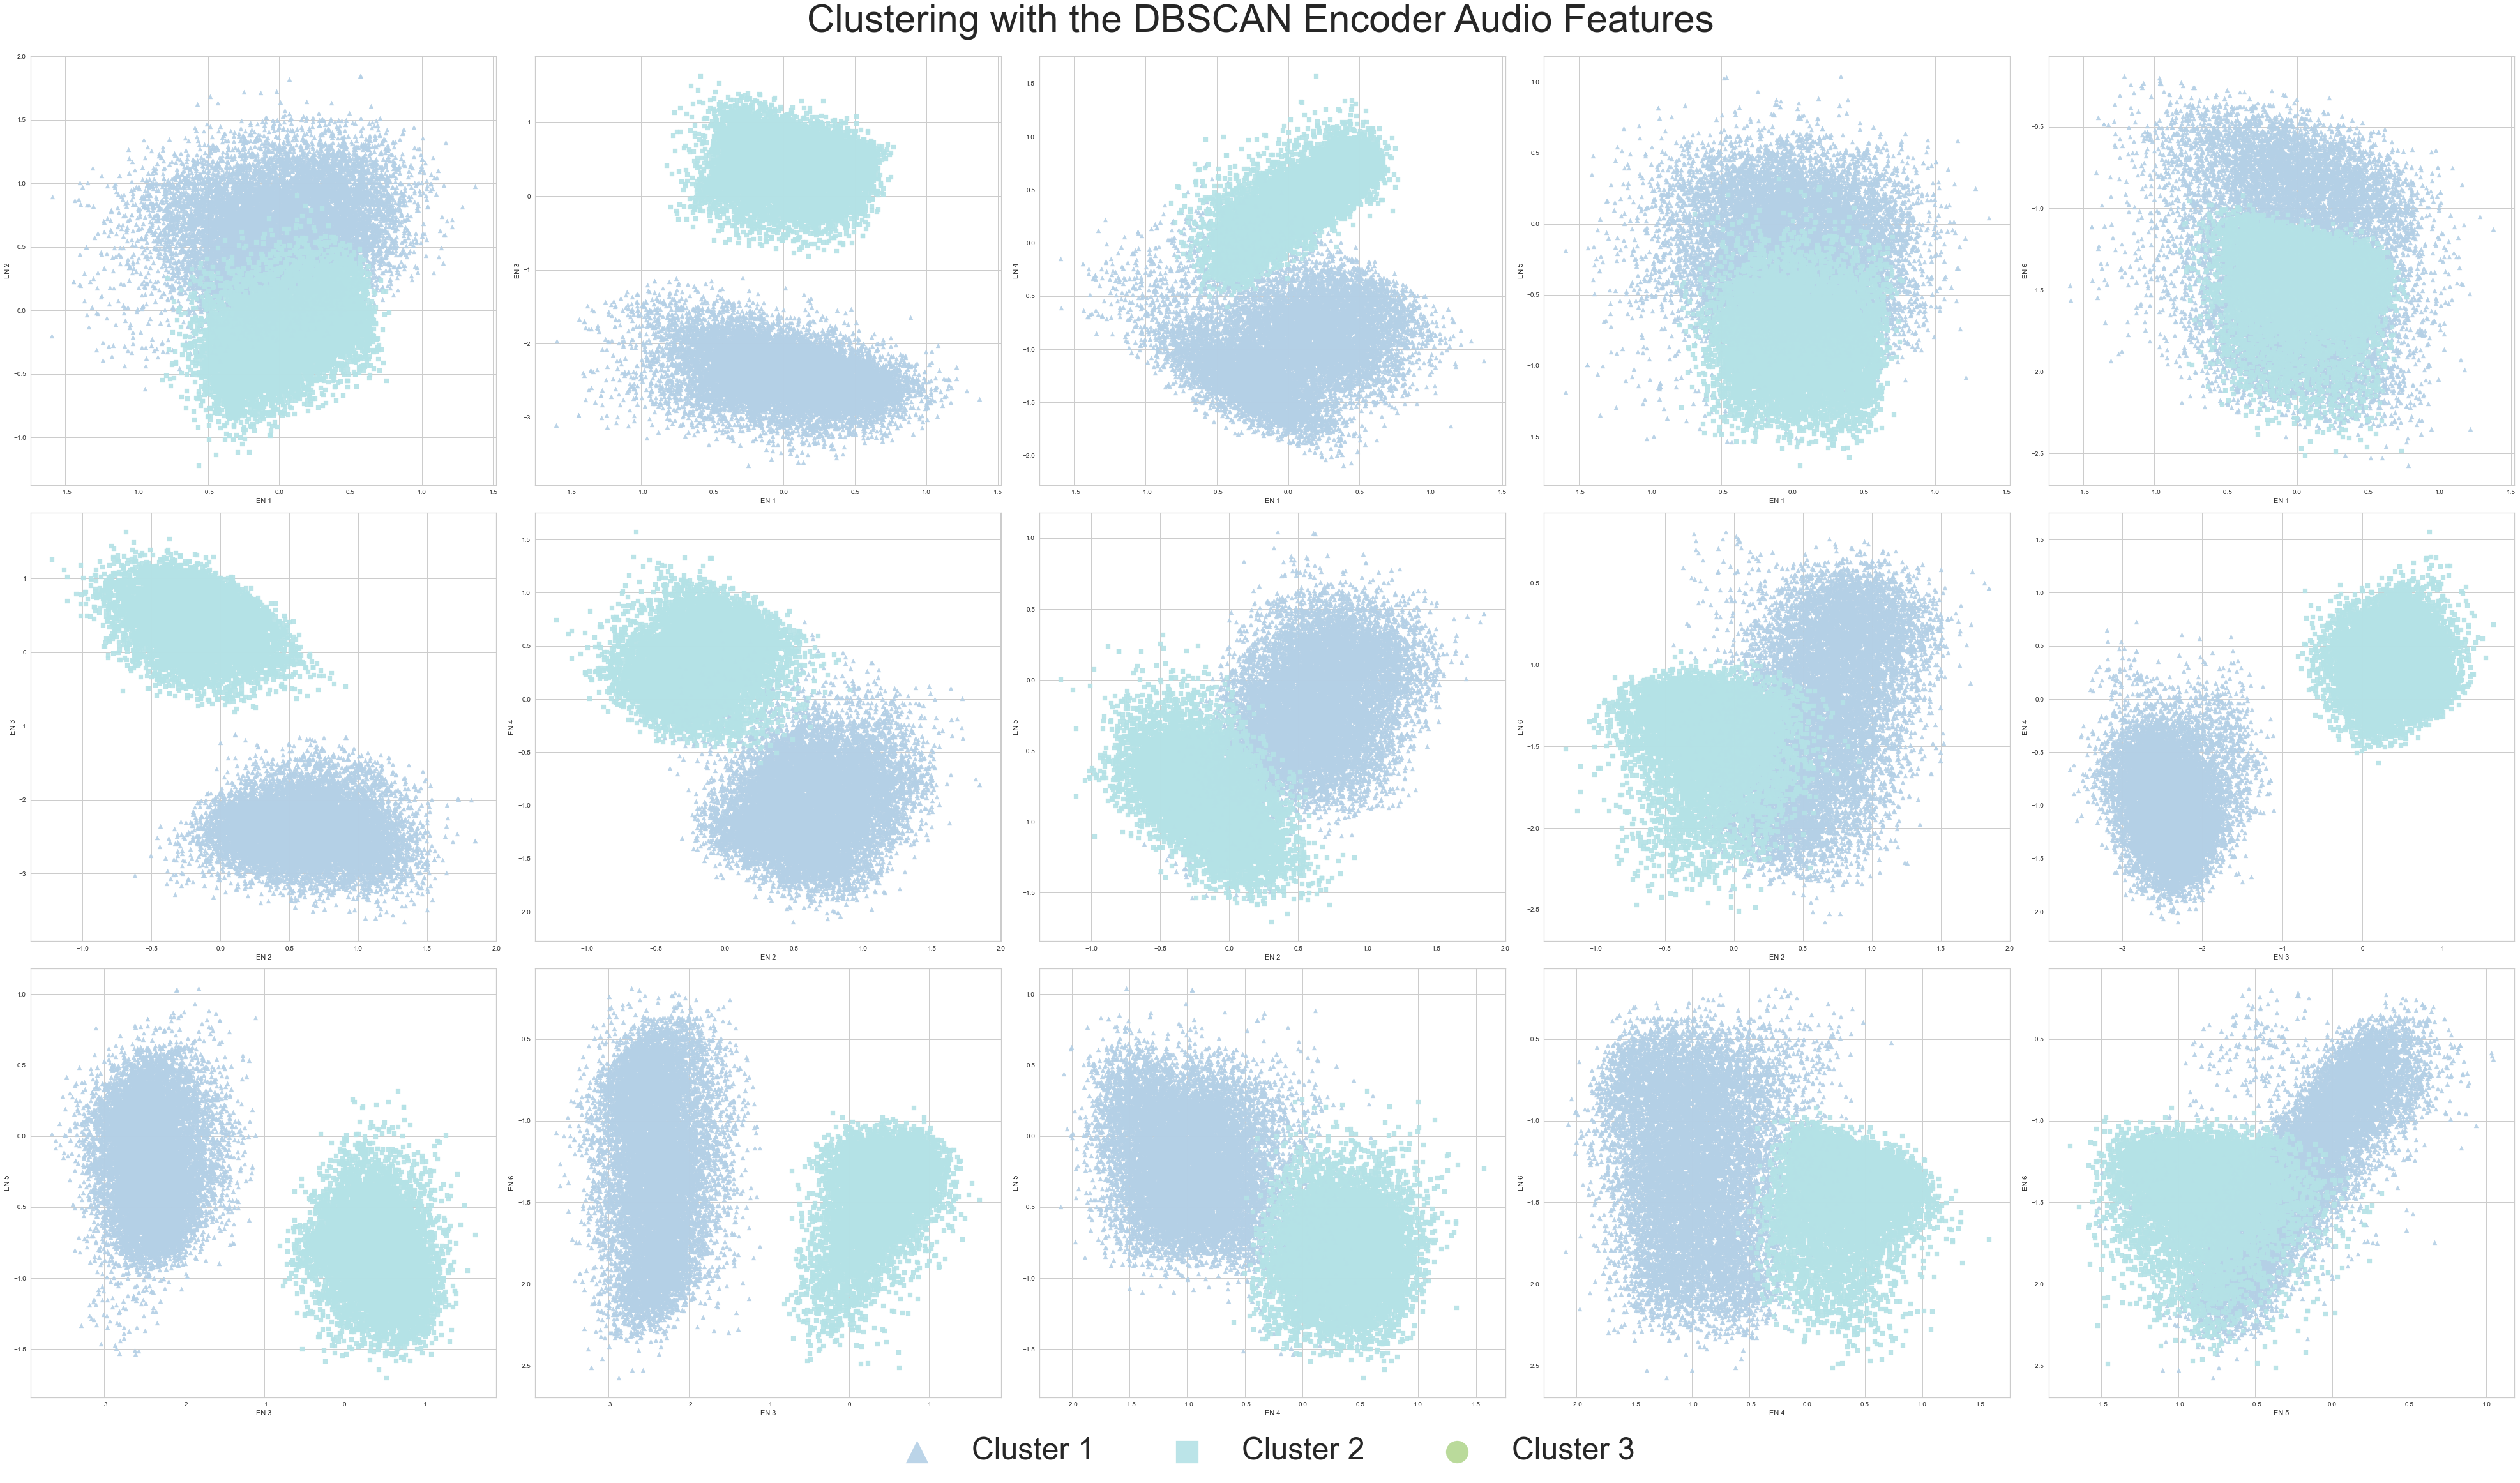
\includegraphics[scale=0.09]{Outputs/DBSCAN Clustering - Autoencoder Audio Features.png}
    \caption{DBSCAN clustering on the Autoencoder derived audio features}
    \label{fig:dbscan-sixth}
\end{figure}
\FloatBarrier
\section{K-Means with PaCMAP Cluster Analysis}
\label{appendix:D}
Some observations from the grid plot reveal that cluster 5 has songs with highest danceability, energy, loudness, valence and tempos while those in cluster 2 are more melodious (as characterised by their low energy and danceability and high acousticness). While the songs in cluster 0 and 1 also contain some rave tracks, the difference lies in their keys, speechiness and skewness of the valence attributes. Cluster 7 is a sparse cluster which contains songs with high instrumentalness.
\begin{figure}[!htb]
    \centering
    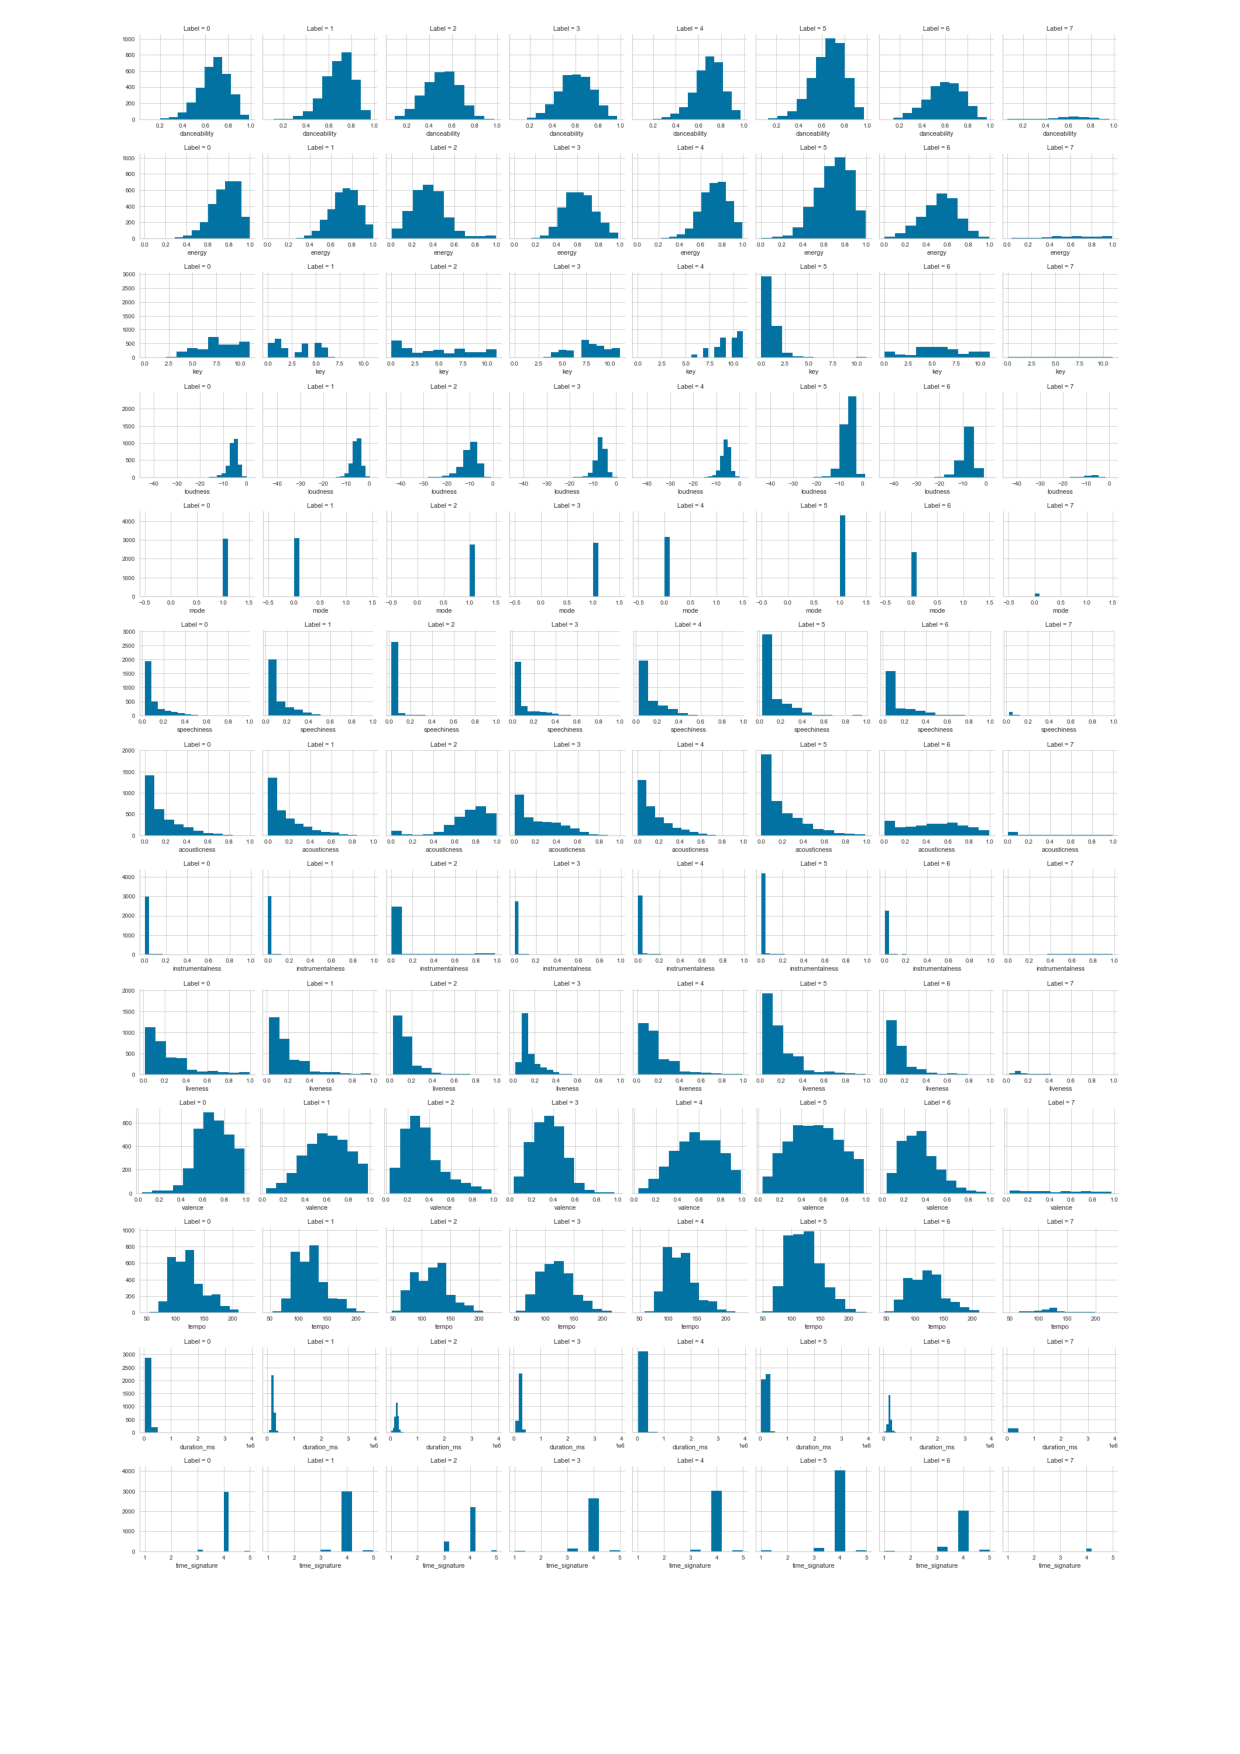
\includegraphics[scale=0.6]{Outputs/Best Algorithm Cluster Analysis.pdf}
    \caption{K-Means with PaCMAP cluster representations in terms of the 13 audio features}
    \label{fig:kmeans-pacmap}
\end{figure}
\clearpage
\section{Artist Clustering}
\label{appendix:E}
\begin{table}[h]
\centering
\begin{tabular}{|l|r|r|r|r|r|r|r|r|r|}
\toprule
{Artist} &    0 &    1 &    2 &    3 &    4 &    5 &    6 &    7 &    8 \\
\midrule
Denki Groove              &  0.0 &  0.0 &  1.0 &  0.0 &  2.0 &  0.0 &  0.0 &  0.0 &  1.0 \\
Marshmello                &  1.0 &  1.0 &  3.0 &  0.0 &  0.0 &  0.0 &  1.0 &  0.0 &  1.0 \\
Rafet El Roman            &  0.0 &  0.0 &  0.0 &  0.0 &  0.0 &  0.0 &  0.0 &  1.0 &  0.0 \\
Katncandix2               &  0.0 &  0.0 &  0.0 &  1.0 &  0.0 &  0.0 &  0.0 &  0.0 &  1.0 \\
Ikke Hüftgold             &  0.0 &  0.0 &  0.0 &  0.0 &  0.0 &  0.0 &  1.0 &  0.0 &  0.0 \\
Beverly                   &  0.0 &  0.0 &  2.0 &  0.0 &  0.0 &  0.0 &  0.0 &  0.0 &  0.0 \\
Kim Churchill             &  1.0 &  0.0 &  0.0 &  0.0 &  0.0 &  0.0 &  0.0 &  0.0 &  0.0 \\
Tim Arisu                 &  0.0 &  0.0 &  1.0 &  0.0 &  0.0 &  0.0 &  0.0 &  0.0 &  0.0 \\
Pitbull                   &  3.0 &  1.0 &  7.0 &  0.0 &  0.0 &  2.0 &  5.0 &  1.0 &  0.0 \\
Savage Garden             &  0.0 &  0.0 &  1.0 &  0.0 &  0.0 &  0.0 &  0.0 &  0.0 &  0.0 \\
Hornet La Frappe          &  0.0 &  7.0 &  2.0 &  0.0 &  5.0 &  0.0 &  1.0 &  7.0 &  0.0 \\
Dengaz                    &  0.0 &  1.0 &  0.0 &  0.0 &  1.0 &  0.0 &  0.0 &  0.0 &  0.0 \\
Snakehips                 &  0.0 &  0.0 &  2.0 &  0.0 &  0.0 &  0.0 &  1.0 &  0.0 &  0.0 \\
Kyle Edwards;Chris Bevrly &  0.0 &  1.0 &  0.0 &  0.0 &  0.0 &  0.0 &  0.0 &  0.0 &  0.0 \\
Andra Day                 &  0.0 &  0.0 &  0.0 &  2.0 &  0.0 &  0.0 &  0.0 &  0.0 &  0.0 \\
IKE                       &  0.0 &  0.0 &  1.0 &  0.0 &  0.0 &  0.0 &  0.0 &  0.0 &  0.0 \\
EXO                   &  2.0 &  1.0 &   6.0 &  2.0 &  4.0 &   1.0 &  3.0 &  2.0 &  3.0 \\
Crowded House             &  0.0 &  1.0 &  0.0 &  0.0 &  0.0 &  0.0 &  0.0 &  0.0 &  0.0 \\
Mitch James               &  0.0 &  0.0 &  0.0 &  1.0 &  0.0 &  1.0 &  0.0 &  0.0 &  0.0 \\
La Combo Tortuga          &  0.0 &  0.0 &  1.0 &  0.0 &  0.0 &  1.0 &  2.0 &  0.0 &  0.0 \\
Alex Rose                 &  0.0 &  0.0 &  0.0 &  0.0 &  1.0 &  0.0 &  0.0 &  0.0 &  0.0 \\
100\%                      &  0.0 &  0.0 &  0.0 &  0.0 &  0.0 &  0.0 &  0.0 &  1.0 &  0.0 \\
MFÖ                       &  1.0 &  0.0 &  0.0 &  0.0 &  0.0 &  0.0 &  0.0 &  0.0 &  0.0 \\
Marianas Trench           &  0.0 &  0.0 &  1.0 &  0.0 &  0.0 &  0.0 &  0.0 &  0.0 &  0.0 \\
Joshua Garcia             &  0.0 &  1.0 &  0.0 &  0.0 &  0.0 &  0.0 &  0.0 &  0.0 &  0.0 \\
Leonardo Lamacchia        &  0.0 &  1.0 &  0.0 &  0.0 &  0.0 &  0.0 &  0.0 &  0.0 &  0.0 \\
Natalie Imbruglia         &  0.0 &  0.0 &  0.0 &  0.0 &  0.0 &  0.0 &  1.0 &  0.0 &  0.0 \\
Crecer German             &  0.0 &  0.0 &  0.0 &  0.0 &  1.0 &  0.0 &  0.0 &  0.0 &  0.0 \\
The xx                    &  0.0 &  1.0 &  0.0 &  4.0 &  5.0 &  0.0 &  1.0 &  1.0 &  3.0 \\
Urban Cone                &  0.0 &  0.0 &  1.0 &  0.0 &  0.0 &  0.0 &  1.0 &  0.0 &  0.0 \\
\bottomrule
\end{tabular}
\end{table}
\section{Clustering using Trends}
\label{appendix:F}
\subsection{Introduction}
The idea here was to cluster songs with a similar trajectories as shown in figure \label{fig:trendstwosongs}. To cluster them by simply feeding in the steaming data for the whole year would make the number of features too high for the clustering model. We used two ways to capture the mathematical information about the trends which were - using the features from the encoder layer of a convolution autoencoder and the transformed features from polynomial regression. 

\begin{figure}[h]
\centering
\centerline{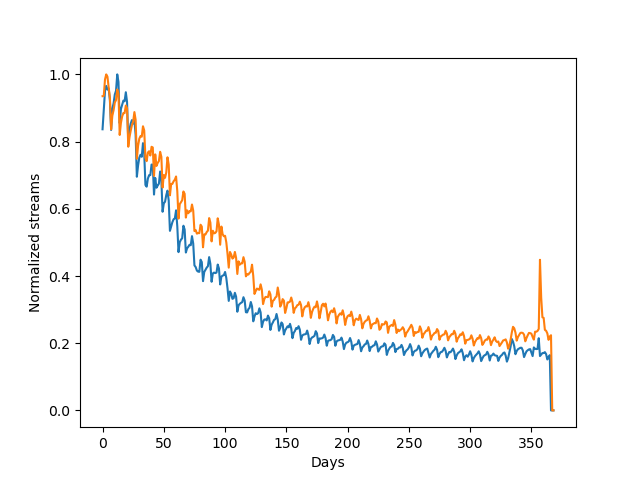
\includegraphics[scale=0.6]{Outputs/cluster example 1.png}}
\caption{Trends of two similar songs}
\label{fig:trendstwosongs}
\end{figure}

\subsection{Data Preparation}
We selected the songs in the global region as they had most number of streams as shown in \label{fig:streamsper}. We used the song's URL as keys for each song, as many songs have the name track name.

\begin{figure}[h]
\centering
\centerline{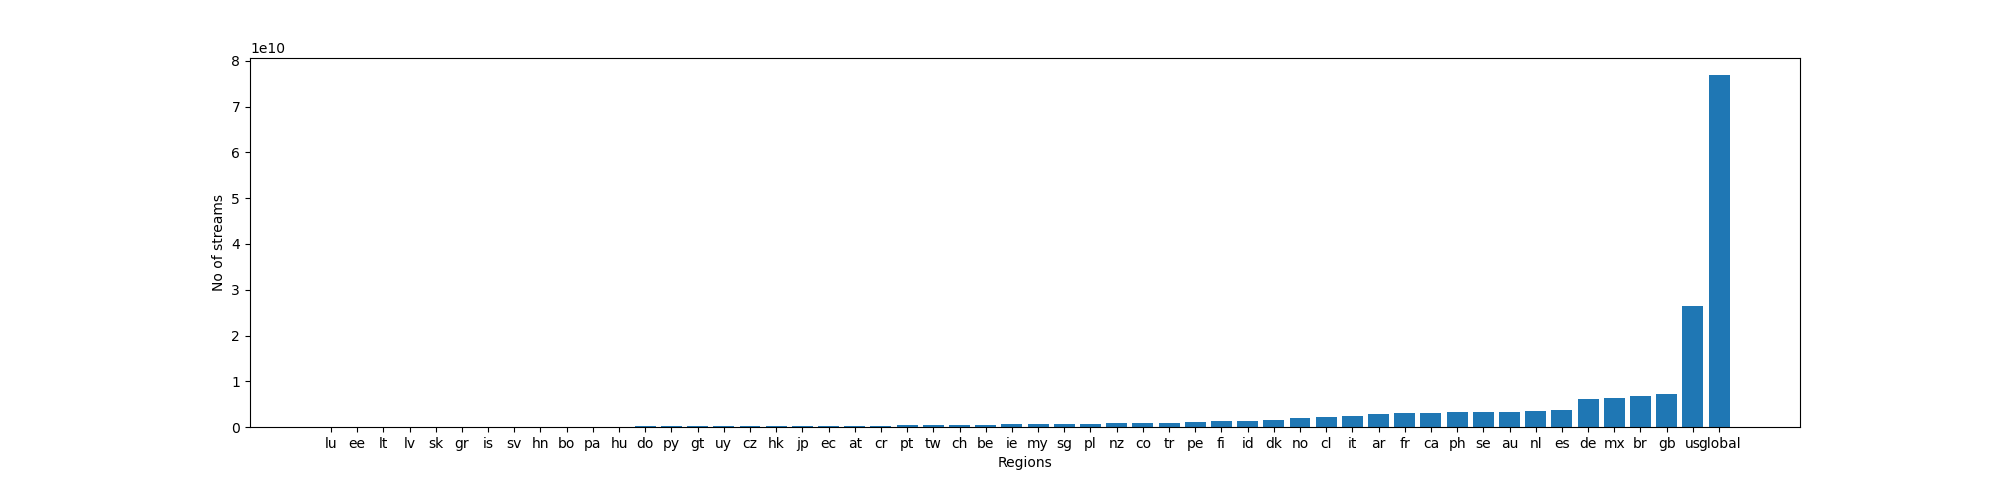
\includegraphics[width=\textwidth]{Outputs/streams per region.png}}
\caption{Barplot of regions with their total streams throughout the year}
\label{fig:streamsper}
\end{figure}

For each song, we fetched the total number of streams and normalised them to the range of [0,1]. We then 0 padded the array for the days the songs were not present in the charts.

\subsection{Methods}
\textbf{Convolutional Autoencoder} - humans use visual features to compare trends - features like shapes and slopes. Convolution Neural Networks work exceptionally well on image classification tasks and just like humans as they can capture visual features like edges and shapes accurately. Using a convolutional autoencoder with the encoded images as features could capture the visual features for the trends of songs.

We converted the streams of each song into trends as images of size 28x28. This image was fed into the convolutional autoencoder and after training, the encoded information of each image were reconstructed. We used the features from the encoder layer for clustering using K-Means. 

\textbf{Polynomial Regression} -
To capture the mathematical features of a trend one can fit a curve to it and use the parameters of the curve as features to define the curve.

For the normalised streams of each song we fit a ploynomial regressor with 5 parameters. There 5 parameters/coefficients were stored and then fed to the K-Means clustering algorithm as its features.

\subsection{Results and Conclusion}
The convolutional autoencoder-based clustering didn't work well as it was just resizing the image and not learning the edges, shapes or any of the other mathematical features from the curves (see \ref{fig:caout}). Also, the encoded features were still in 2 dimensions, so these features lost the relationships to its nearby pixels when flattened, and the number of features were still too high for the clustering algorithm to work with.

\begin{figure}[h]
\centering
\centerline{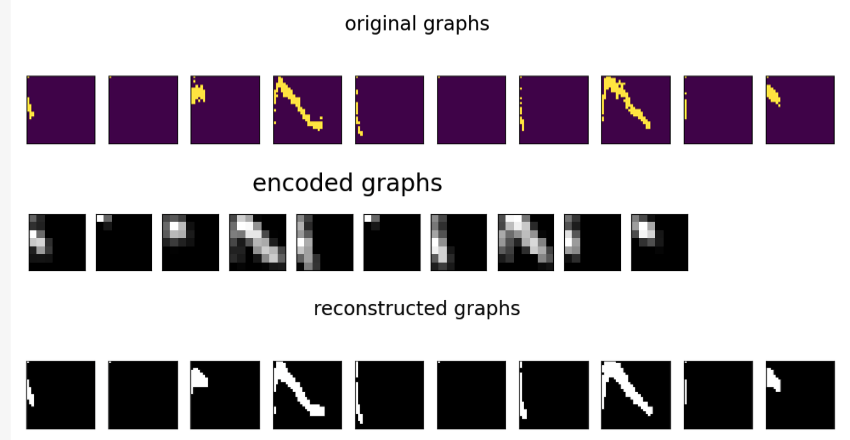
\includegraphics[width=\textwidth]{Outputs/caout.png}}
\caption{Output of the trends from the encoder layer}
\label{fig:caout}
\end{figure}
The polynomial feature-based clustering was able to cluster similar trends together as shown in \label{fig:polyout} . But, it could not cluster similar trends for songs which lasted on the charts for different number of days. The results are tabluated in \ref{tab:table4}

For this to work, we would need the complete data, i.e. all the songs, should have data for each day of the year. Or if we have labels for the cluster, i.e. if we could train in a supervised manner, then a classification algorithm will be able to match songs with similar trends irrespective of the days that it lasts on the charts.
\begin{figure}[h]
\centering
\centerline{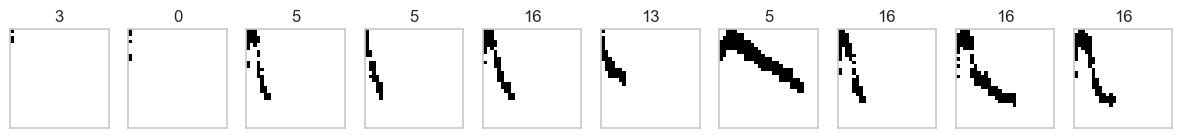
\includegraphics[width=\textwidth]{Outputs/resultploy.png}}
\caption{Trends and their cluster labels after polynomial regressor based clustering with K-Means}
\label{fig:polyout}
\end{figure}

\begin{table}[!hbt]
    \centering
    \rowcolors{1}{white}{gray!25}
    \resizebox{\columnwidth}{!}{%
    \begin{tabular}{|c|c|c|c|c|c|c|}
    \toprule
     \makecell{Clustering \\ Algorithm} & \makecell{Feature Engineering}  & \makecell{No. Clusters} & \makecell{No. Features} & 
     \makecell{CH} & \makecell{DB} & \makecell{SS} \\
    \midrule
        K-Means  & Convolutional Autoencoder      &  12      & 49    & 377.00    & 1.381  & 0.401\\
        K-Means  &  Polynomial Regressor     &  20     & 5     & 6427.71    & 0.748   & 0.527\\
    \bottomrule
    \end{tabular}%
    }
    \caption{Experiment results for the two feature engineering methods with K-Means. SS is silhouette score, DB is Davies–Bouldin index, CH is Calinski Harabasz score.}
    \label{tab:table4}
\end{table} 
\end{appendix} 
\clearpage
\section*{Statement of Contribution}
s2420055 - EDA (acoustic features), Dimensionality Reduction (PCA, Autoencoders), DBSCAN
s2428072 - EDA (trends), Dimensionality Reduction (Gaussian Random Projections, UMAP), BIRCH
s2446690 - Extended data set, EDA (region-wise data), Dimensionality Reduction (PaCMAP), K-Means

Equal contribution in trend based clustering
\end{document}

%%% Local Variables:
%%% mode: latex
%%% TeX-master: t
%%% End:
